\documentclass[14pt,a4paper]{report}  %紙張設定
\usepackage{xeCJK}%中文字體模組
%\setCJKmainfont{標楷體} %設定中文字體
\setCJKmainfont{MoeStandardKai.ttf}
%\newfontfamily\sectionef{Times New Roman}%設定英文字體
\newfontfamily\sectionef{Nimbus Roman}
\usepackage{enumerate}
\usepackage{amsmath,amssymb}%數學公式、符號
\usepackage{amsfonts} %數學簍空的英文字
\usepackage{graphicx, subfigure}%圖形
\usepackage{fontawesome5} %引用icon
\usepackage{type1cm} %調整字體絕對大小
\usepackage{textpos} %設定文字絕對位置
\usepackage[top=2.5truecm,bottom=2.5truecm,
left=3truecm,right=2.5truecm]{geometry}
\usepackage{titlesec} %目錄標題設定模組
\usepackage{titletoc} %目錄內容設定模組
\usepackage{textcomp} %表格設定模組
\usepackage{multirow} %合併行
%\usepackage{multicol} %合併欄
\usepackage{CJK} %中文模組
\usepackage{CJKnumb} %中文數字模組
\usepackage{wallpaper} %浮水印
\usepackage{listings} %引用程式碼
\usepackage{hyperref} %引用url連結
\usepackage{setspace}
\usepackage{lscape}%設定橫式
\lstset{language=Python, %設定語言
		basicstyle=\fontsize{10pt}{2pt}\selectfont, %設定程式內文字體大小
		frame=lines,	%設定程式框架為線
}
%\usepackage{subcaption}%副圖標
\graphicspath{{./../images/}} %圖片預設讀取路徑
\usepackage{indentfirst} %設定開頭縮排模組
\renewcommand{\figurename}{\Large 圖.} %更改圖片標題名稱
\renewcommand{\tablename}{\Large 表.}
\renewcommand{\lstlistingname}{\Large 程式.} %設定程式標示名稱
\hoffset=-5mm %調整左右邊界
\voffset=-8mm %調整上下邊界
\setlength{\parindent}{3em}%設定首行行距縮排
\usepackage{appendix} %附錄
\usepackage{diagbox}%引用表格
\usepackage{multirow}%表格置中
%\usepackage{number line}
%=------------------更改標題內容----------------------=%
\titleformat{\chapter}[hang]{\center\sectionef\fontsize{20pt}{1pt}\bfseries}{\LARGE 第\CJKnumber{\thechapter}章}{1em}{}[]
\titleformat{\section}[hang]{\sectionef\fontsize{18pt}{2.5pt}\bfseries}{{\thesection}}{0.5em}{}[]
\titleformat{\subsection}[hang]{\sectionef\fontsize{18pt}{2.5pt}\bfseries}{{\thesubsection}}{1em}{}[]
%=------------------更改目錄內容-----------------------=%
\titlecontents{chapter}[11mm]{}{\sectionef\fontsize{18pt}{2.5pt}\bfseries\makebox[3.5em][l]
{第\CJKnumber{\thecontentslabel}章}}{}{\titlerule*[0.7pc]{.}\contentspage}
\titlecontents{section}[18mm]{}{\sectionef\LARGE\makebox[1.5em][l]
{\thecontentslabel}}{}{\titlerule*[0.7pc]{.}\contentspage}
\titlecontents{subsection}[4em]{}{\sectionef\Large\makebox[2.5em][l]{{\thecontentslabel}}}{}{\titlerule*[0.7pc]{.}\contentspage}
%=----------------------章節間距----------------------=%
\titlespacing*{\chapter} {0pt}{0pt}{18pt}
\titlespacing*{\section} {0pt}{12pt}{6pt}
\titlespacing*{\subsection} {0pt}{6pt}{6pt}
%=----------------------標題-------------------------=%             
\begin{document} %文件
\sectionef %設定英文字體啟用
\vspace{12em}
\begin{titlepage}%開頭
\begin{center}   %標題  
\makebox[1.5\width][s] %[s] 代表 Stretch the interword space in text across the entire width
{\fontsize{24pt}{2.5pt}國立虎尾科技大學}\\[18pt]
\makebox[1.5\width][s]
{\fontsize{24pt}{2.5pt}機械設計工程系}\\[18pt]
\sectionef\fontsize{24pt}{1em}\selectfont\textbf
{
\vspace{0.5em}
cd2023 2b3-pj3bg6分組報告}\\[18pt]
%設定文字盒子 [方框寬度的1.5倍寬][對其方式為文字平均分分布於方框中]\\距離下方18pt
\vspace{1em} %下移
\fontsize{30pt}{1pt}\selectfont\textbf{網際足球場景設計}\\
\vspace{1em}
\sectionef\fontsize{30pt}{1em}\selectfont\textbf
{
\vspace{0.5em}
Web-based Foosball Scene Design}
 \vspace{2em}
%=---------------------參與人員-----------------------=%             
\end{center}
\begin{flushleft}
\begin{LARGE}

\hspace{32mm}\makebox[5cm][s]
{指導教授:\quad 嚴\quad 家\quad 銘\quad 老\quad 師}\\[6pt]
\hspace{32mm}\makebox[5cm][s]
{班\qquad 級:\quad 四\quad 設\quad 二\quad 乙}\\[6pt]
\hspace{32mm}\makebox[5cm][s]
{學\qquad 生:\quad 莊\quad 雨\quad 薰\quad(41023203)}\\[6pt]
\hspace{32mm}\makebox[5cm][s]
{\hspace{36.5mm}陳\quad 妤\quad 瑄\quad(41023204)}\\[6pt]
\hspace{32mm}\makebox[5cm][s]
{\hspace{36.5mm}陳\quad 靚\quad 芸\quad(41023205)}\\[6pt]
\hspace{32mm}\makebox[5cm][s]
{\hspace{36.5mm}陳\quad 澤\quad 瑜\quad(41023206)}\\[6pt]
\hspace{32mm}\makebox[5cm][s]
{\hspace{36.5mm}楊\quad 舒\quad 涵\quad(41023207)}\\[6pt]
\hspace{32mm}\makebox[5cm][s]
{\hspace{36.5mm}廖\quad 子\quad 儀\quad(41023208)}\\[6pt]
\hspace{32mm}\makebox[5cm][s]
{\hspace{36.5mm}鄭\quad 翊\quad 均\quad(41023210)}\\[6pt]
\hspace{32mm}\makebox[5cm][s]
{\hspace{36.5mm}徐\quad 佑\quad 寧\quad(41023255)}\\[6pt]

%設定文字盒子[寬度為5cm][對其方式為文字平均分分布於方框中]空白距離{36.5mm}\空白1em
\end{LARGE}
\end{flushleft}
\vspace{6em}
\fontsize{18pt}{2pt}\selectfont\centerline{\makebox[\width][s]
{中華民國\hspace{3em} 
112 \quad 年\quad 6\quad 月}}
\end{titlepage}
\newpage
%=------------------------摘要-----------------------=%
\renewcommand{\baselinestretch}{1.5} %設定行距
\pagenumbering{roman} %設定頁數為羅馬數字
\clearpage  %設定頁數開始編譯
\sectionef
\addcontentsline{toc}{chapter}{摘~~~要} %將摘要加入目錄
\begin{center}
\LARGE\textbf{摘~~要}\\
\end{center}
\begin{flushleft}
\fontsize{14pt}{20pt}\sectionef\hspace{12pt}\quad 由於矩陣計算、自動求導技術、開源開發環境、多核GPU運算硬體等這四大發展趨勢,促使AI領域快速發展,藉由這樣的契機,將實體機電系統透過虛擬化訓練提高訓練效率,再將訓練完的模型應用到實體上。\\[12pt]

\fontsize{14pt}{20pt}\sectionef\hspace{12pt}\quad 此專題是運用實體冰球對打機,將其導入CoppeliaSim模擬環境並給予對應設置,將其機電系統簡化並運用Open AI Gym進行訓練,找到適合此系統的演算法後,再到CoppeliaSim模擬環境中進行測試演算法在實際運用上的可行性。並嘗試透過架設伺服器將CoppeliaSim影像串流到網頁供使用者觀看或操控。\\[12pt]

\end{flushleft}
\begin{center}
\fontsize{14pt}{20pt}\selectfont 關鍵字: 類神經網路、強化學習、\sectionef CoppeliaSim、OpenAI Gym
\end{center}
\newpage
%=--------------------Abstract----------------------=%
\renewcommand{\baselinestretch}{1.5} %設定行距
\addcontentsline{toc}{chapter}{Abstract} %將摘要加入目錄
\begin{center}
\LARGE\textbf\sectionef{Abstract}\\
\begin{flushleft}
\fontsize{14pt}{16pt}\sectionef\hspace{12pt}\quad Due to the four major development trends of multidimensional arrays  computing, automatic differentiation, open source development environment, and multi-core GPUs computing hardware. The rapid development of the AI field has been promoted. In view of this development, the physical mechatronic systems can gain machine learning efficiency through their simulated virtual system training process. And afterwards to apply the trained model into real mechatronic systems.\\[12pt]

\fontsize{14pt}{16pt}\sectionef\hspace{12pt}\quad This project is to use the physical air hockey to play machine, introduce it into the CoppeliaSim simulation environment and give the corresponding settings, simplify its electromechanical system and use Open AI Gym for training, find an algorithm suitable for this system, and then perform it in the CoppeliaSim simulation environment Feasibility of testing algorithm in practical application. And try to stream CoppeliaSim images to web pages for users to watch or manipulate by setting up a server.\\
\end{flushleft}
\begin{center}
\fontsize{14pt}{16pt}\selectfont\sectionef Keyword:  nerual network、reinforcement learning、 CoppeliaSim、OpenAI Gym
\end{center}

\newpage
%=------------------------目錄----------------------=%
\renewcommand{\contentsname}{\centerline{\fontsize{18pt}{\baselineskip}\selectfont\textbf{目\quad 錄}}}
\tableofcontents  %目錄產生
\newpage
%=------------------圖表目錄產生----------------------=%
\renewcommand{\listfigurename}{\centerline{\fontsize{18pt}{\baselineskip}\selectfont\textbf{圖\quad 目\quad 錄 }}}
\newcommand{\loflabel}{圖} %定義\loflabel 文字為圖
\renewcommand{\numberline}[1]{\loflabel~#1\hspace*{0.5em}}
\listoffigures
%\newcommand{\captioname}{圖}
\newpage
\renewcommand{\listtablename}{\centerline{\fontsize{18pt}{\baselineskip}\selectfont\textbf{表\quad 目\quad 錄 }}}
\newcommand{\lotlabel}{表} %定義\lotlabel 文字為表
\renewcommand{\numberline}[1]{\lotlabel~#1\hspace*{0.5em}}
\listoftables

\end{center}
%=-------------------------內容----------------------=%
\chapter{前言}
\renewcommand{\baselinestretch}{10.0} %設定行距
\pagenumbering{arabic} %設定頁號阿拉伯數字
\setcounter{page}{1}  %設定頁數
\fontsize{14pt}{2.5pt}\sectionef
\section{研究動機}
機器學習與各領域結合的應用越來越廣泛,在機電系統採用強化學習是為了讓機電系統的控制達到最佳化。本專題以實體的冰球機(圖.\ref{fig.冰球機})之機電系統作為訓練模型,將實體機器轉移到虛擬環境(圖.\ref{fig.模擬冰球機})進行模擬,為了找到適合的訓練參數,因此將模型簡化(圖.\ref{fig.pong_gym})後再進行測試各種參數的優劣,透過不斷的訓練來得到一個優化過的對打系統。\\

\begin{figure}[hbt!]
\begin{center}
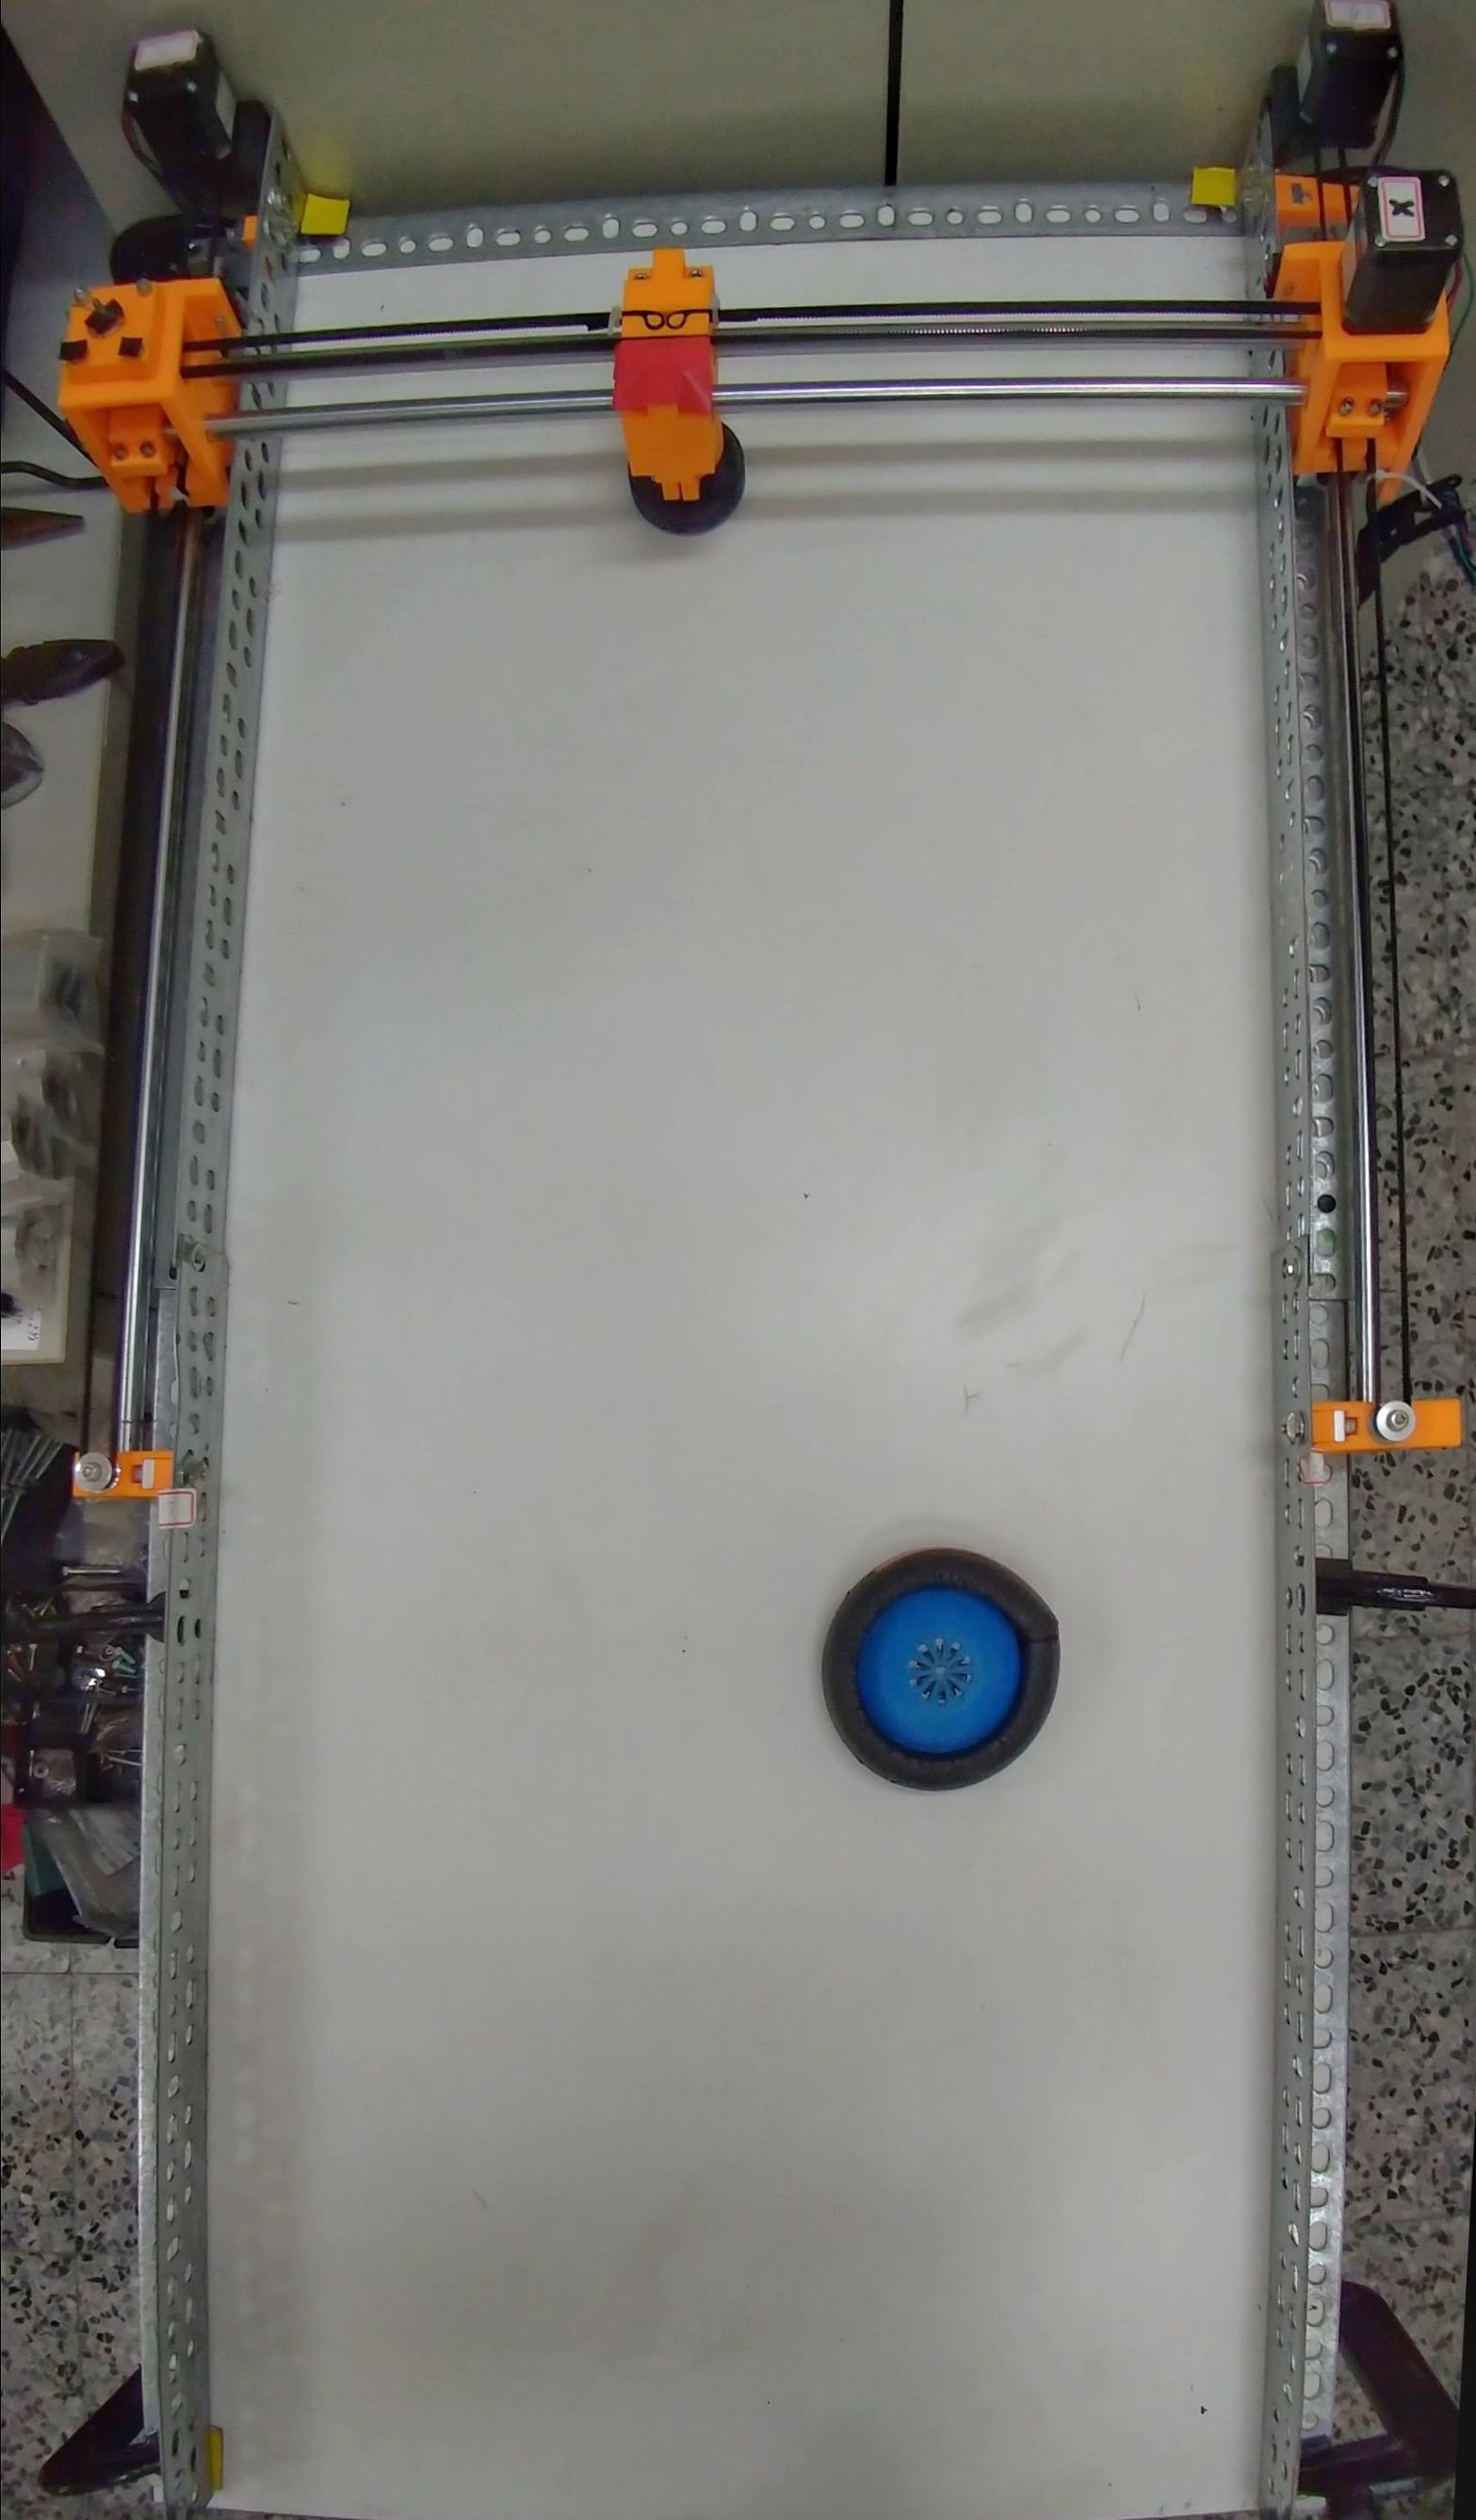
\includegraphics[angle=90,width=10cm]{冰球機}
\caption{\Large 實體的冰球機}\label{fig.冰球機}
\end{center}
\end{figure}
\begin{figure}[hbt!]
\begin{center}
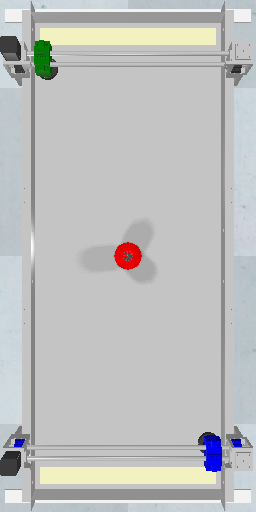
\includegraphics[angle=90,width=10cm]{origin}
\caption{\Large 虛擬環境簡化後的冰球機}\label{fig.模擬冰球機}
\end{center}
\end{figure}
\begin{figure}[hbt!]
\begin{center}
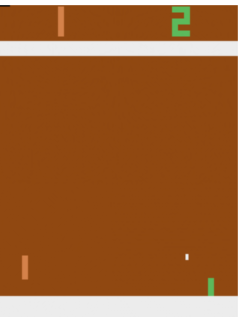
\includegraphics[height=8cm]{pong_gym}
\caption{\Large Gym的Pong game}\label{fig.pong_gym}
\end{center}
\end{figure}


\section{研究目的與方法}
本研究分三大部分,第一運用OpenAI Gym裡內建編譯的ATARI 2600遊戲Pong-v0,來作為訓練環境,加上強化學習的理論,測試不同演算法參數以訓練出最佳化的對打系統,第二將整個簡化後冰球機導入CoppilaSim模擬環境並嘗試進行虛擬訓練,成為優化的對打機電系統。第三則是嘗試透過架設伺服器與虛擬環境結合。\\
 
透過簡化實體冰球機並導入虛擬環境,進行虛擬訓練,使用Gym的Pong當作對應的2D虛擬訓練環境,測試算法和訓練效果,篩選適合的算法與參數。\\

建置CoppilaSim模擬環境,嘗試將2D訓練概念套用到3D環境進行測試,加入電腦視覺與RemoteAPI,電腦視覺抓取球與擊錘的位置,透過RemoteAPI進行遠端控制,在3D環境測試算法可確保後續套用到實體機器上的可行性。\\
 
 再透過架設伺服器與虛擬環境結合:讓虛擬環境的影像透過網伺服器串流影像供使用者遠端進行操控虛擬環境的擊錘進行打球,或是提供多人進行觀看對打影像。
\begin{figure}[hbt!]
\begin{center}
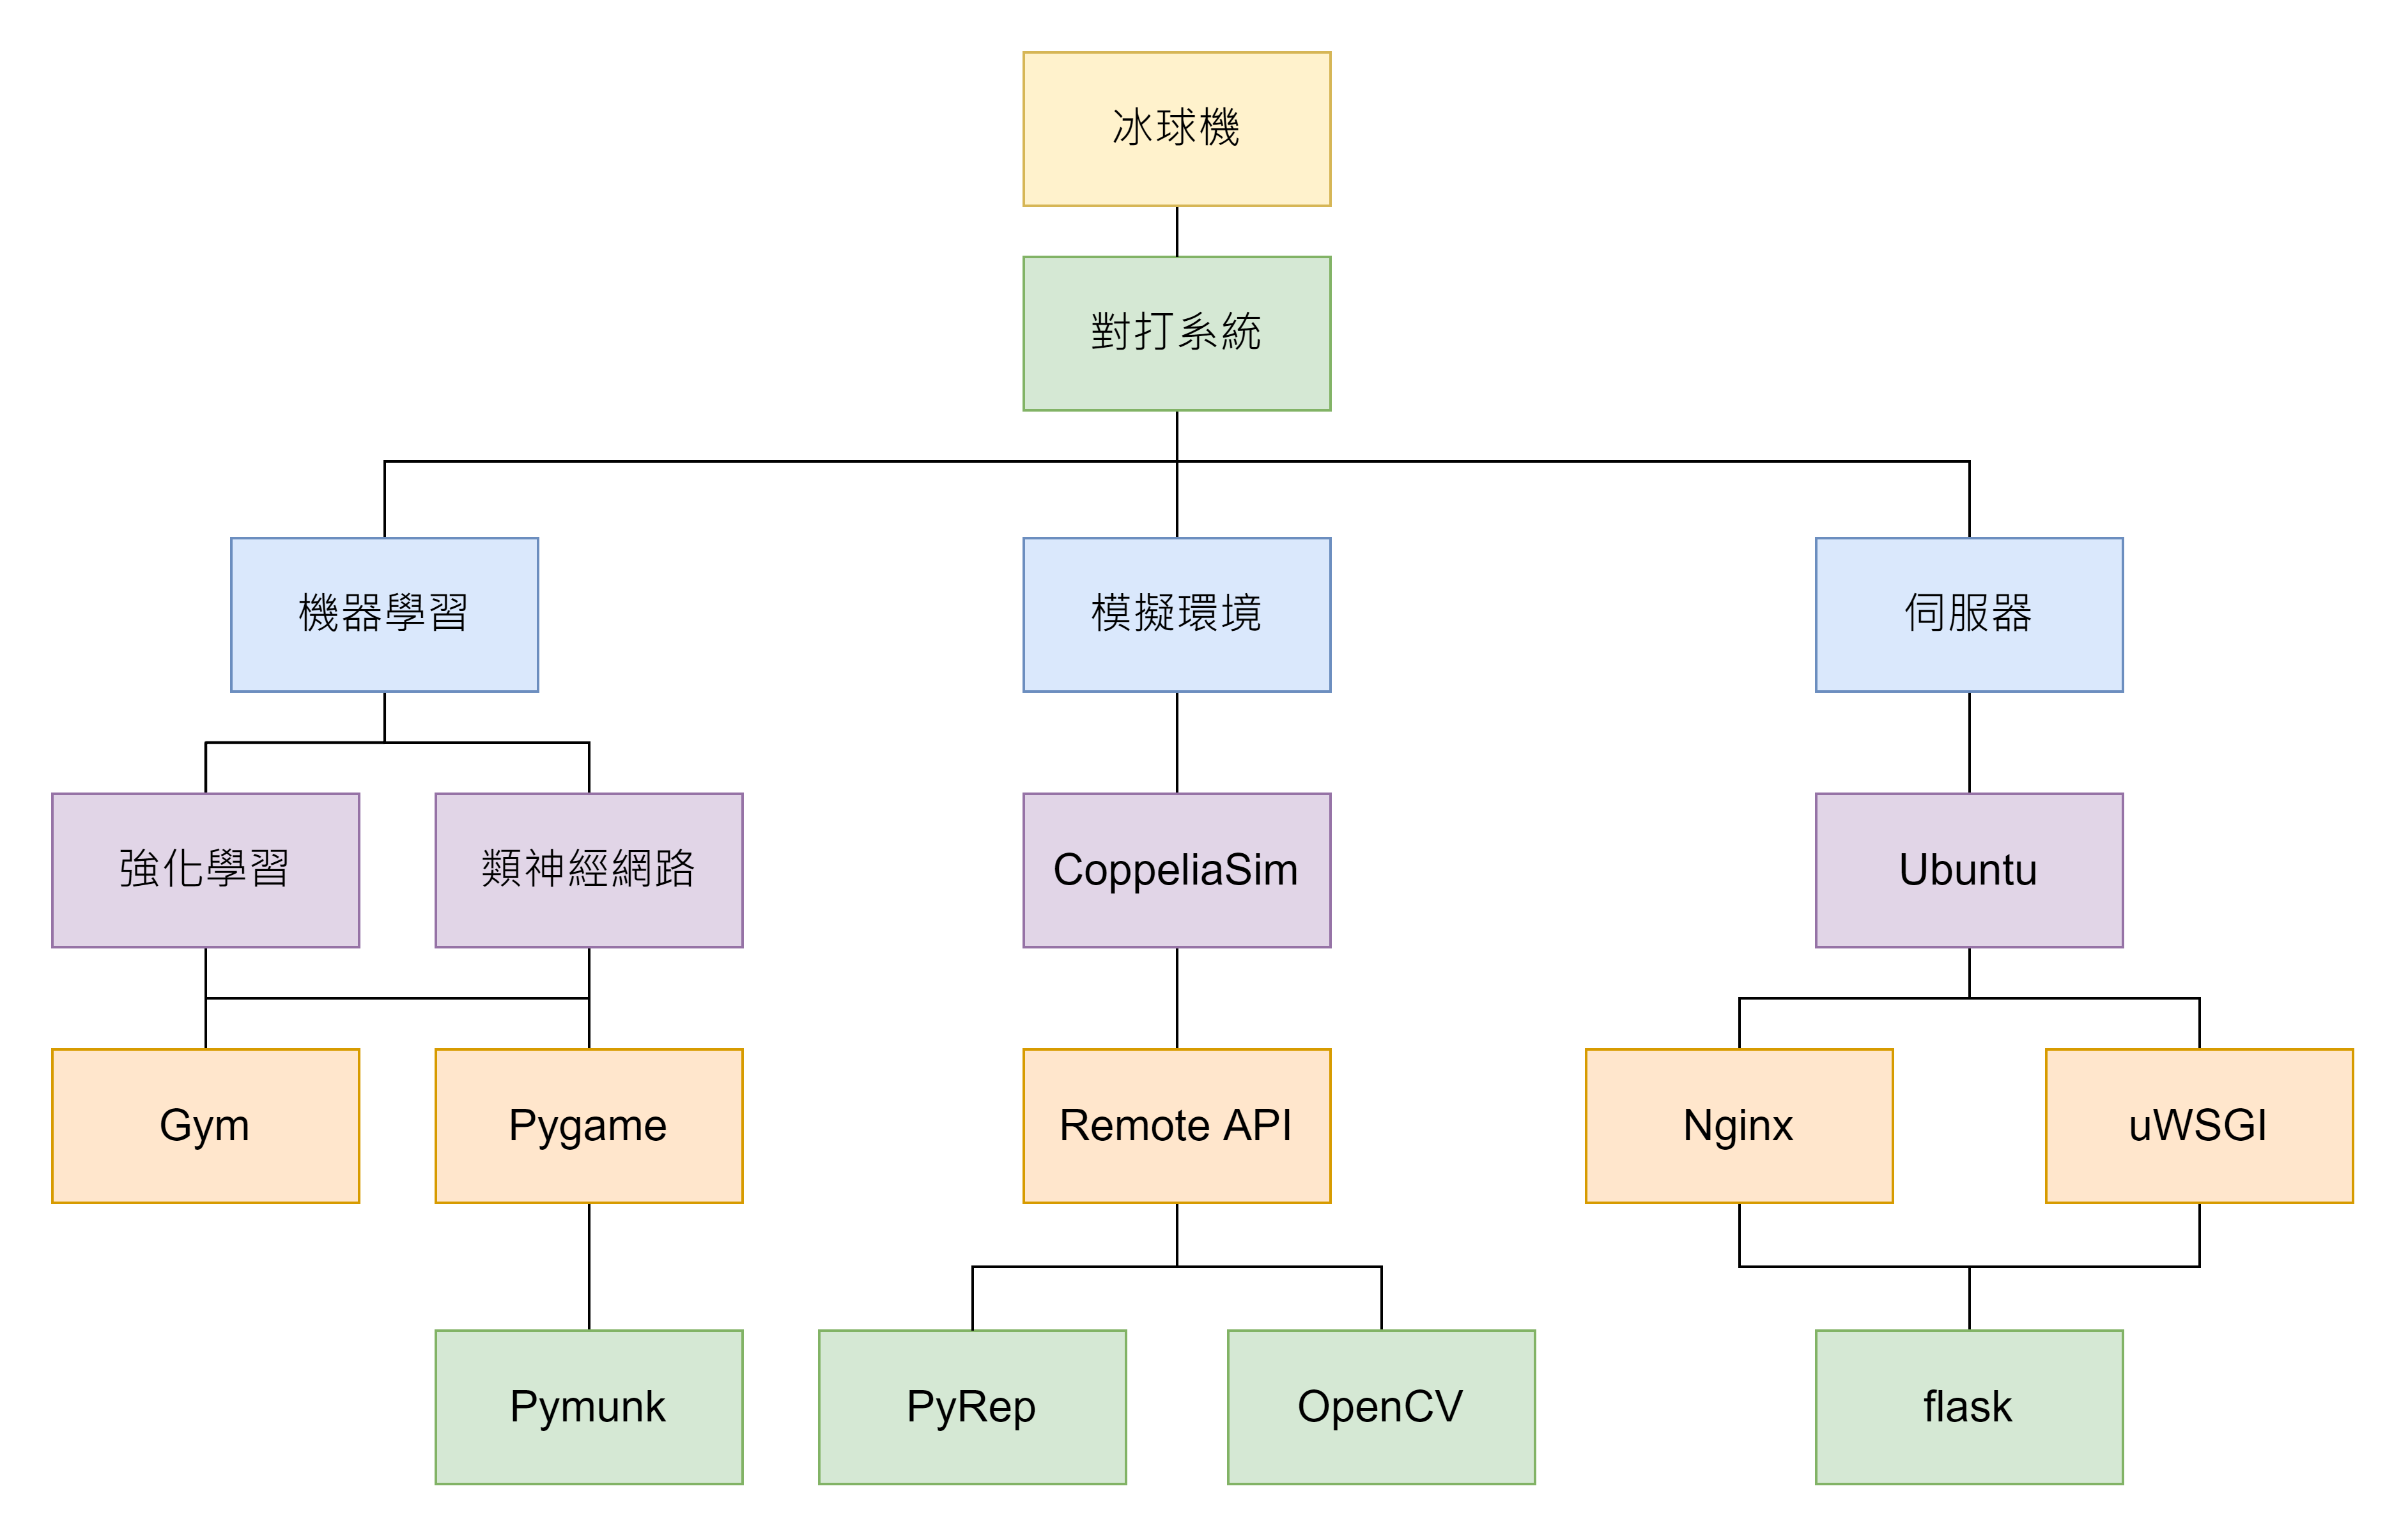
\includegraphics[width=15cm]{研究架構}
\caption{\Large 研究架構 }
\label{研究架構 }
\end{center}
\end{figure}
\section{未來展望}
此專題希望能利用現有完成的機械學習的算法,能發展成虛擬訓練,再將訓練完的機器學習應用到虛擬環境或是實體機電系統,並透過伺服器將影像串流提供玩家網頁介面進行遠端操控,同時提供多人觀看及時的比賽影像,將整個冰球機的控制和使用者間有更完善串聯,機電系統的部分達到最優化控制和虛實整合的應用。
\section{規則說明}
 Pong game 的遊戲規則簡單,透過擊錘將球打入對方球門即得一分,只要其中一方得21分就結束該局。擊錘只能沿單方向來回移動來進行防守和進攻。\\
遊戲規則如下:
\begin{enumerate}
\item 球打入敵方即得一分。
\item 擊錘只單一方向移動。
\item 最快贏得21分者獲勝,並結束該局遊戲。
\end{enumerate}

\renewcommand{\baselinestretch}{0.5} %設定行距
\chapter{機器學習}
\section{類神經網絡}
\begin{figure}[hbt!]
\begin{center}
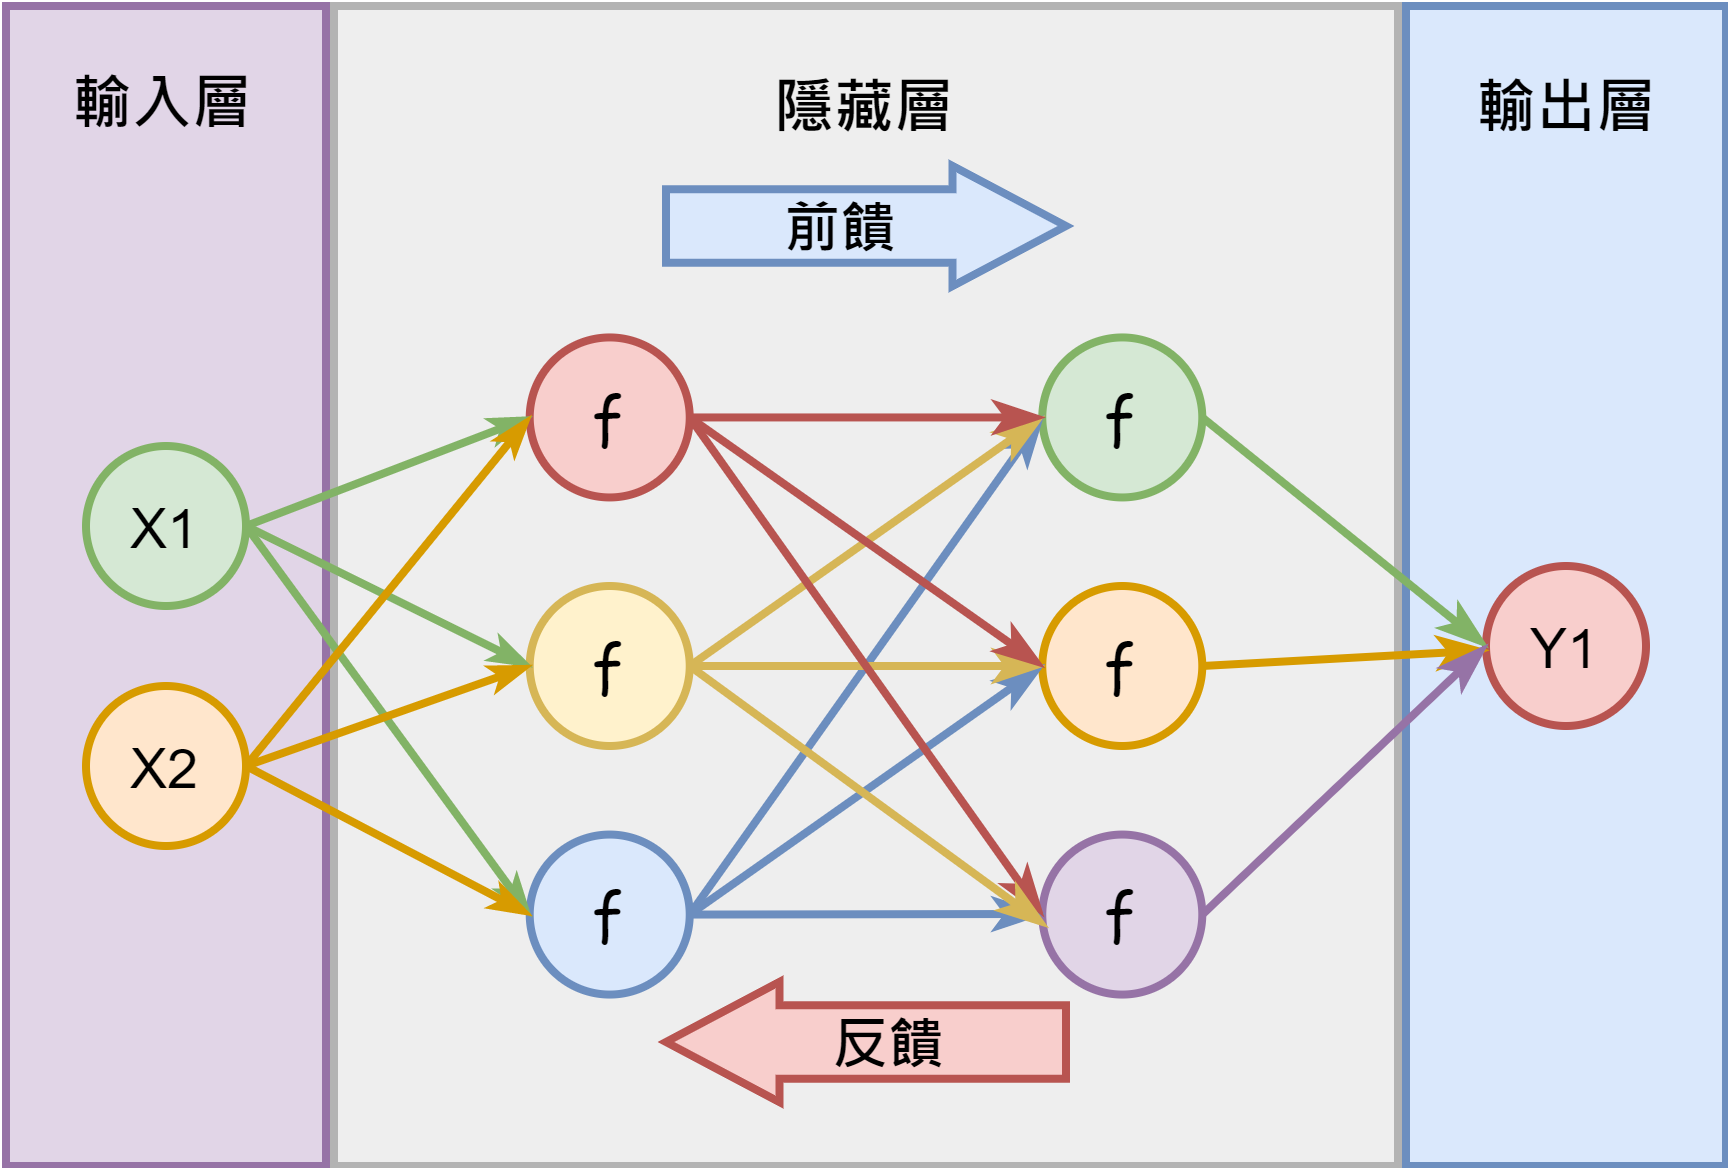
\includegraphics[width=16cm]{類神經網路架構}
\caption{\Large 類神經網路架構}\label{類神經網路架構}
\end{center}
\end{figure}

 典型的類神經網路架構,如(圖.\ref{類神經網路架構})所示每一層的每一個神經元都會連接到下一層全部的神經元,對於每個神經元輸出會有不同的權重。\\

 神經元是AI系統中使用的數學模型,其行為與實際的大腦神經元運作方式相仿,模型以數字的方式表達,神經元間傳遞會有不同強度,而以數值的大小代表不同強度,這個數值我們稱為權重,對結果產生重要的影響。\\

 (圖.\ref{類神經網路架構})基礎的類神經網路架構主要由輸入層、隱藏層和輸出層這三部分組成,實際運用上還有更多樣更複雜的類神經網路架構,深度學習則是有更多的隱藏層,從意義上來說就是增加了類神經網路的深度。\\

 此外,如(圖.\ref{類神經網路架構})所示,資料由輸入層傳入,經過隱藏層運算和記憶,再由輸出層進行輸出,這種資料被傳遞的方式被稱為前饋輸入(feed-forward)。\\

 類神經網路架構有了記憶,就能進一步讓網路學習。當類神經網路接收資料並猜測答案,如果答案與實際答案不符、有落差或有錯誤的情況,它會回授並修改對每個神經元權重和偏差修正的程度,並嘗試調配各項數值來修正輸出的結果,讓結果的正確性提高,這樣的修正行為就被稱為反向傳播(back-propagation)。透過迭代方法進行反複試驗,模擬人們學習的行為,而每一次的迭代被稱為epoch,經過一定的迭帶次數後會透過反向傳播修正輸出的誤差,經過不斷執行的修正,最終類神經網路的學習會不斷進步並給出更好的答案,訓練時間長短取決於訓練項目的複雜程度。\\

 可以看到該神經網絡的輸出僅取決於互連的權重,還取決於神經元本身的偏差,雖然權重會影響啟動函數曲線的陡度,但是偏差會將發生變化的整個曲線,向右或向左,權重和偏差的選擇,決定了單個神經元的預測強度,而訓練類神經網絡使用的輸入數據可以來微調權重和偏差。(圖.\ref{類神經網路關係})\\

\newpage
\begin{figure}
\begin{center}
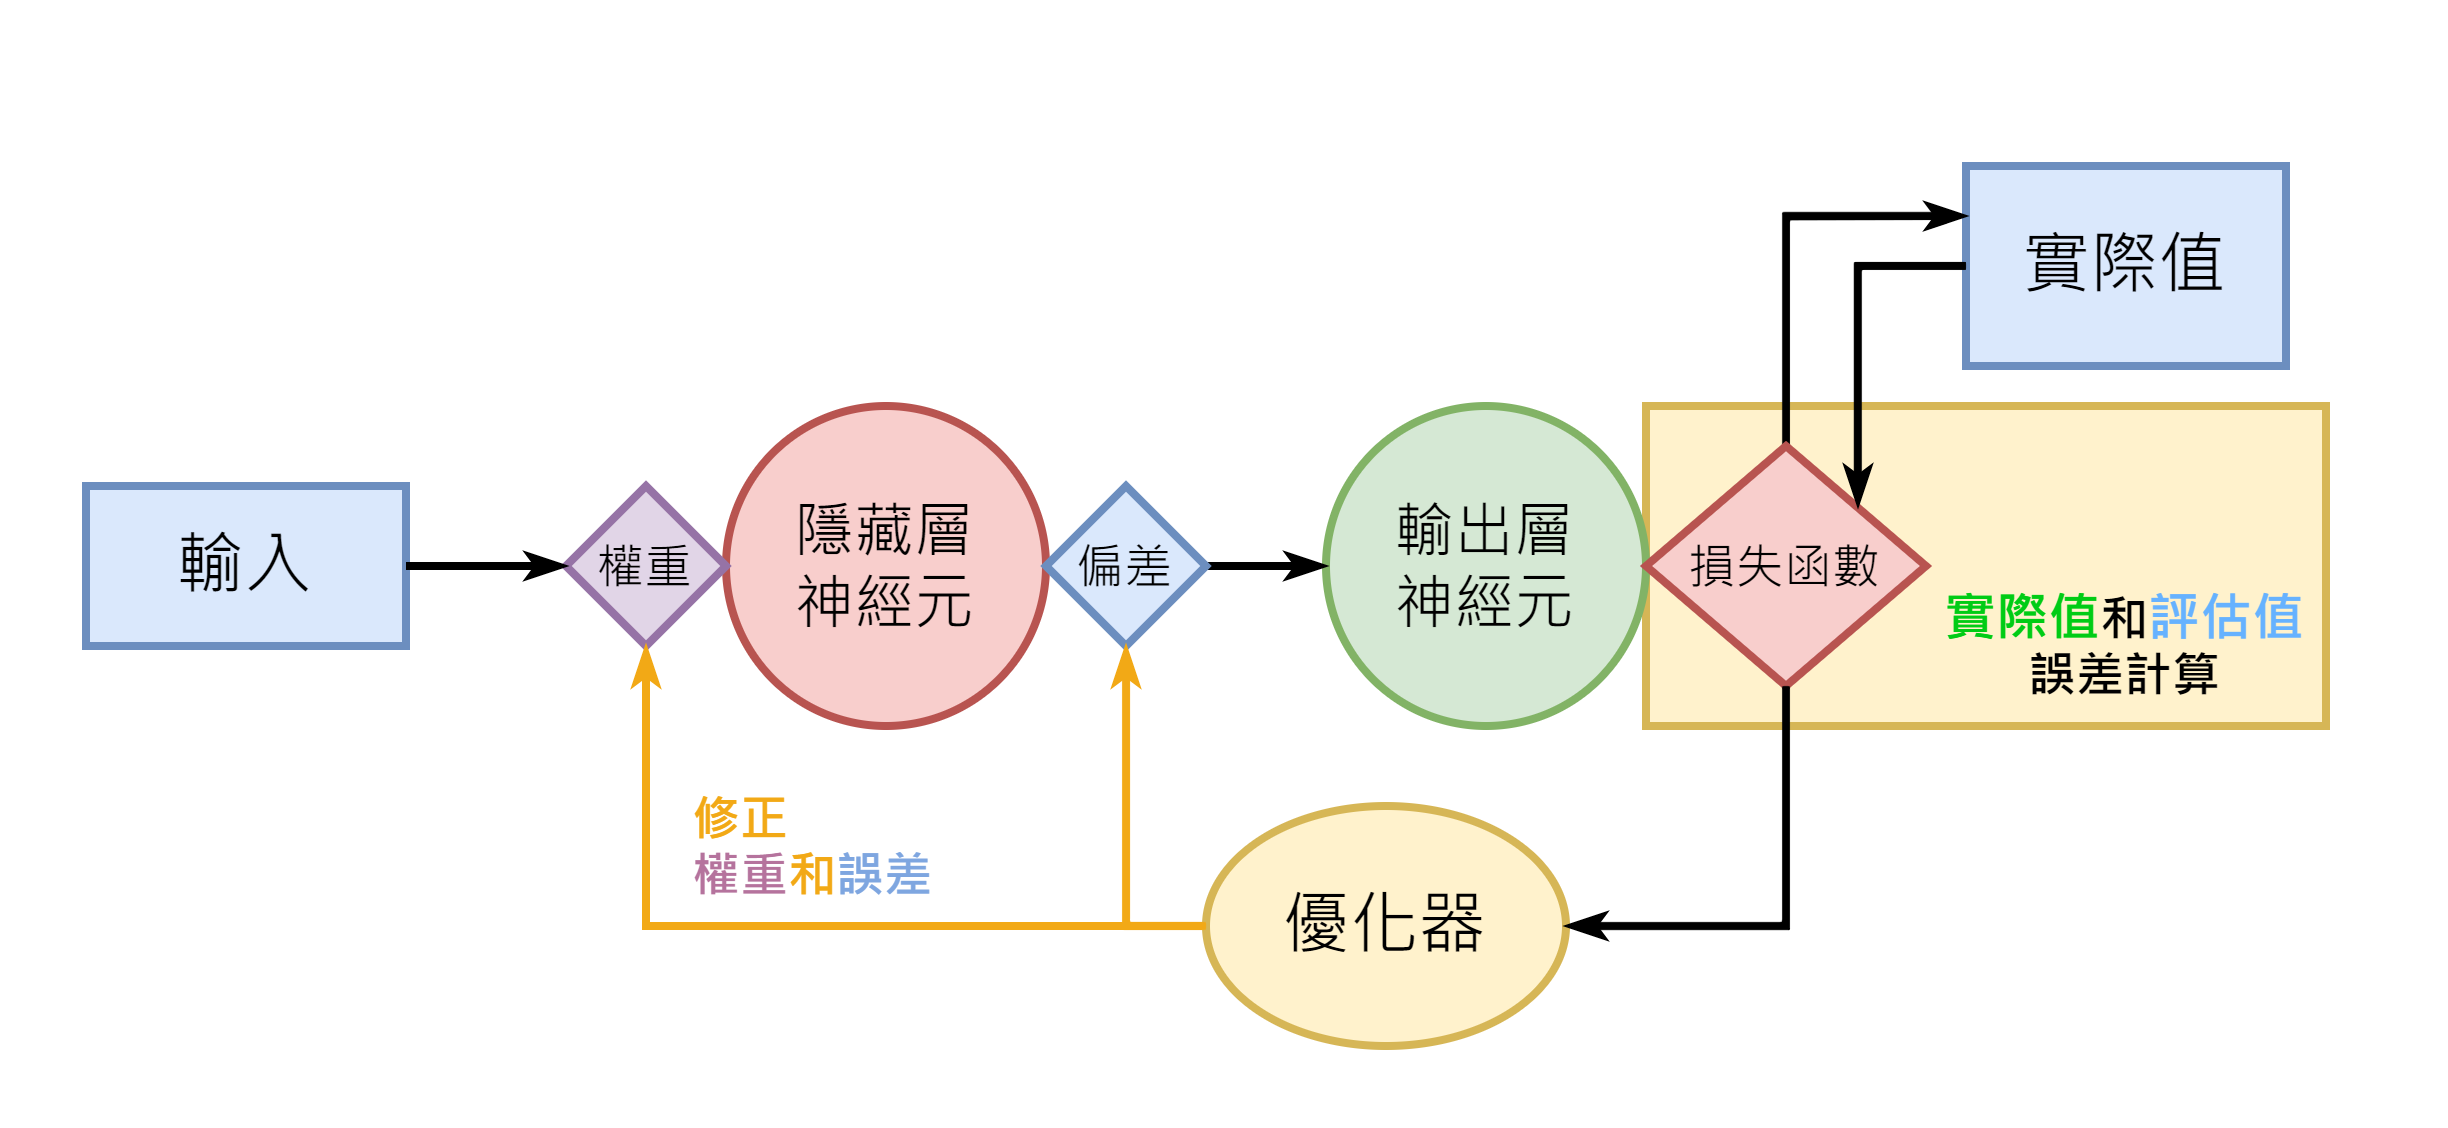
\includegraphics[width=16cm]{類神經網路關係}
\caption{\Large 類神經網路關係}
\label{類神經網路關係}
\end{center}
\end{figure}
\subsection{啟動函數}
啟動函數是設計類神經網路的關鍵部分,如果不使用啟動函數,神經元的計算只會有線性組合,這樣的類神經網路缺乏活性而且記憶性差;啟動函數能讓神經元計算呈現非線性,讓類神經網路因為計算的非線性而提高整個網路的活性和記憶性。\\
以下介紹幾種較為常見的啟動函數及其特性:
\begin{itemize}
%=----------Sigmoid      Function----------=%
\item Sigmoid Function(圖.\ref{SigmoidFunction}):\\
輸出介於0到1之間,適用於二元分類,方程式具有非線性、可連續微分、且具有固定輸出範圍等特性,並可以讓類神經網路呈現非線性。
$$\sigma(x)=\frac{1}{1+e^{-x}}$$

%=----------SigmoidPrime Function----------=%
SigmoidPrime Function(圖.\ref{SigmoidFunction},紅色的)是從Sigmoid Function(圖.\ref{SigmoidFunction},藍色)微分得來,以梯度運算的方式,可以減少梯度誤差,但也是造成梯度消失的主要原因,若要改善梯度消失需要搭配優化器使用,方程式如下:\\
$$\sigma^{'}(x)=\sigma(x)[1-\sigma(x)]$$
\begin{figure}[hbt!]
\begin{center}
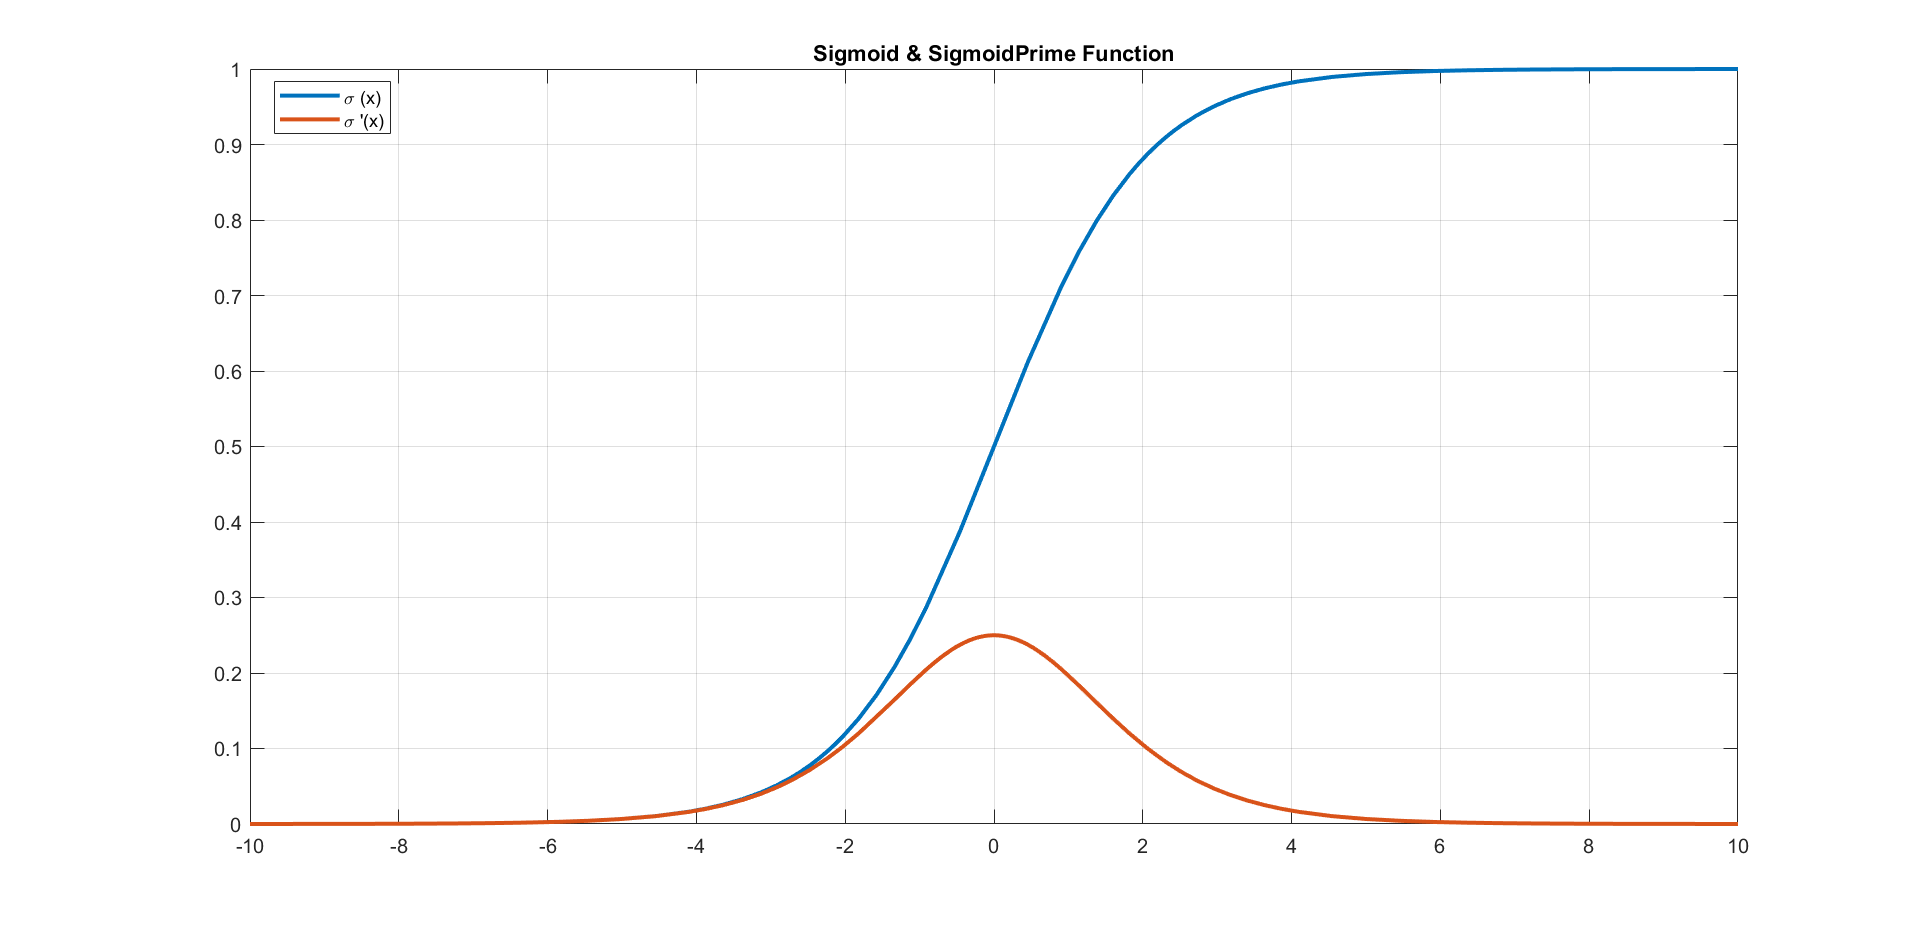
\includegraphics[width=16cm]{SigmoidFunction}
\caption{\Large SigmoidFunction}\label{SigmoidFunction}
\end{center}
\end{figure}
\\
%=----------Softmax Function----------=%
\item Softmax:\\
Softmax會計算每個事件分布的機率,適用多項目分類、其機率總合為1。以此專案為例,假設擊錘移動有向上移動、向下移動及不移動這三個決策選項,則這三個決策機率值總和為1。\\
$$S(x)=\frac{e^{x_i}}{\sum^k_{j=1}e^{x_i}}$$
%=----------Relu Function----------=%
\item ReLU Function:\\
ReLU Function方程式特性:若輸入值為負值,輸出值為0;若輸入值為正值,輸出則維持該輸入數值。ReLU計算方式簡單、收斂速度快,這是類神經網路最普遍拿來使用的啟動函數,因為可以解決梯度消散的問題,但須注意:起始值若設定到不易被激活範圍或是權重過渡所導致權重梯度為0就會造成神經元難以被激活。\\
\end{itemize}
$$f(x)=max(0,x)$$
$$if , x<0 , f(x)=0$$
$$else f(x)=x$$
\subsection{損失函數}
損失函數是類神經網路的另一個重要的部分,損失函數會將類神經網絡的結果與期望結果進行比較,且必須重複估算模型當前狀態的誤差;該函數可用於估計模型的損失,以便可以更新權重減少下次評估時的損失,下一節會有詳細說明,以下簡述幾種優化的方法:\\
\begin{itemize}
\item Gradient Descent\\
利用梯度的方式尋找最小值的位置,其特色可找到凸面error surface的絕對最小值,在非凸面error surface上找到相對最小值。其缺點是在非凸面error surface要避免被困在次優的局部最小值。
\item Batch gradient descent\\
用批次的方式計算訓練資料,整個資料集計算梯度只更新一次,因此計算和更新時會占用大量記憶體。整體效率較差、速度較緩慢。由 Gradient Descent 延伸出來的算法。其收斂行為與 Gradient Descent 相同。
\item Stochastic gradient descent\\
每次執行時會更新並消除誤差,有頻繁更新和變化大的特性,較不容易困在特定區域。由 Gradient Descent 延伸出來的算法。其收斂行為與 Gradient Descent 相同。
\item Mini-batch gradient descent\\
結合 Batch gradient descent 和 Stochastic gradient descent 的特點:批量計算和頻繁更新,所衍伸的算法。利用小批量的方式頻繁更新,並使收斂更穩定。其缺點:學習率挑選不易、預定義 threshold 無法適應數據集的特徵、對很少發生的特徵無法執行較大的更新、非凸面error surface要避免被困在次優的局部最小值等。
\item Gradient descent optimization algorithms\\
為了改善前面幾種算法而發展出來的優化算法。以下將列出數種優化算法。
\item Momentum\\
在梯度下降法加上動量的概念,會加速收斂到最小值並減少震盪。
\item Nesterov accelerated gradient\\
NAG,有感知能力的 Momentum:在坡度變陡時減速,避免衝過最小值所造成的震盪(為了修正到最小值,來回修正而產生的震盪)。
\item Adagrad\\
其學習率能適應參數:頻繁出現的特徵用較低的學習率,不經常出現的特徵則用較高的學習率,且無須手動調整學習率。其缺點是,學習率會急遽下降,最後會無限小,這算法就不再獲得知識。
\item Adadelta\\
為 Adagrad 的延伸,下降激進程度,學習率從更新規則中淘汰,不需設定預設學習率。
\item RMSprop\\
為了解決 Adagrad 學習率急劇下降的問題,學習率除以梯度平方的RMS,解決學習率無限小的情形。
\item Adam Function\\
結合了 Adagrad 和 RMSprop的優勢,有論文表示,在訓練速度方面有巨大性的提升,但在某些情況下,Adam實際上會找到比隨機梯度下降法更差的解決方法。以下是計算過程:\\
$$g_t=\delta_{\theta}f(\theta)$$
一次矩指數移動均線 :\\
$$m_t =\beta(m_{t-1})+(1-\beta_1)(\nabla{w_t})$$
$$\hat m_t=\frac{m_t}{1-\beta_1^t}$$
二次矩指數移動均線 :\\
$$v_t=\beta_2(v_t-1)+(1-\beta_2)(\nabla{w_t})^2$$
$$\hat{v_t}=\frac{v_t}{1-\beta_2^t}$$
因此,Adam Function:\\
$$\omega_{t-1}=\omega_t-\frac{\eta}{\sqrt{\hat{v_t}-\epsilon}}\hat{m_t}$$
\item AdaMax\\
與 Adam 相似,依靠$(u_t)$ 最大運算。
\item Nadam\\
結合 Adam 和 NAG ,應用先前參數執行兩次更新,一次更新參數一次更新梯度。
\item AMSGrad\\
改善 Adam 算法所導致收斂較差的情況(用指數平均會減少其影響),換用梯度平方最大值來做計算,並移除去偏差的步驟。是否有比 Adam 算法好仍有待觀察。
\item Gradient noise\\[6pt]
有助於訓練特別深且復雜的網絡,noise 可改善不良初始化的網路。
\item Mean Squared Error\\
他能告訴你一組點與回歸線接近的程度,透過獲取點與回歸線之距離(這些距離就是誤差)並對它們進行平方來做到這點,而平方是為了消除所有負號,也能讓更大的差異賦予更大的權重。\\
\vspace{8cm}
\begin{figure}
\begin{center}
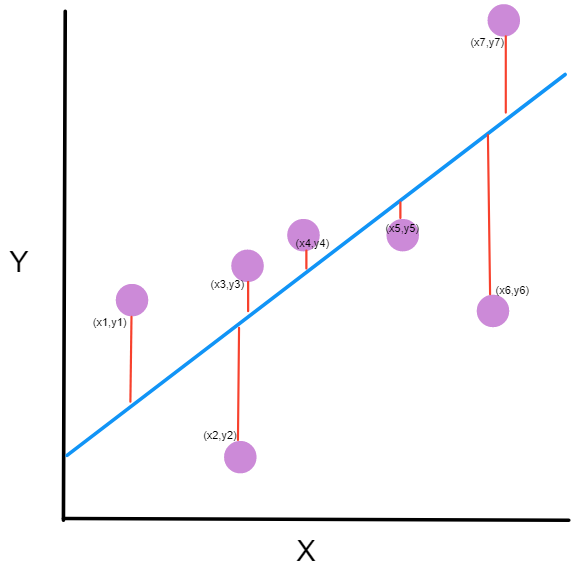
\includegraphics[scale=0.6]{MSE}
\caption{\Large 線性回歸}\label{線性回歸}
\end{center}
\end{figure}
\qquad \\

回歸線 :數據點間最小距離的一條線。 \\
n:數據點的數量\\
$y_i$: 觀測值\\
$\hat{y_i}$:預測值\\
$$MSE=\frac{1}{n} \sum_{i=1}^n(y_i-\overline{y} _i)^2$$\\
\end{itemize}
\newpage
\subsection{優化算法}
\renewcommand{\baselinestretch}{1}

\begin{itemize}
\item Gradient Descent Optimizer[\ref{OGD}]\\

\begin{figure}[hbt!]
\begin{center}
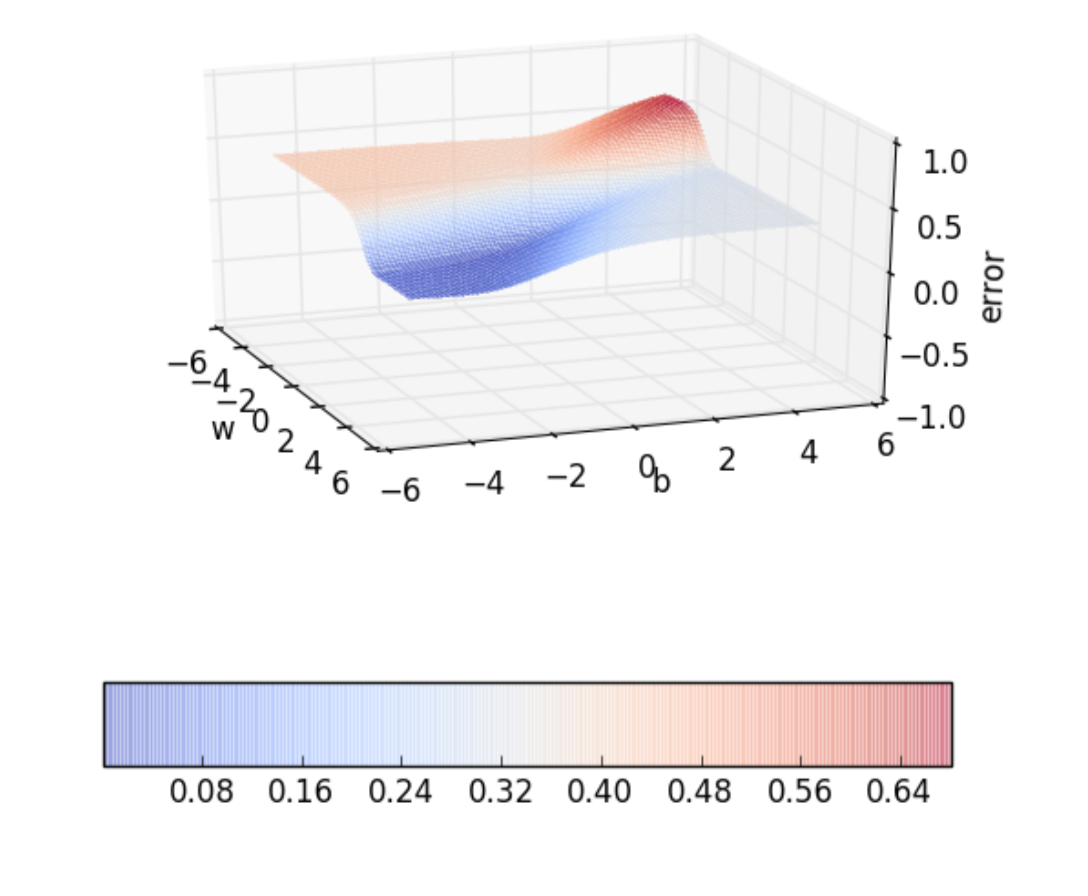
\includegraphics[width=10cm]{Error_surface-2}
\caption{\Large Error surface [\ref{OGD}]}
\label{Error_surface-2}
\end{center}
\end{figure}
%\fontsize{14pt}{28pt}\selectfont
 藉由梯度下降將目標函數值最小化,目標函數以loss function L($\theta$)為例,$\theta$為weight(w)和bias(b)的向量函數,為了找到(圖.\ref{Error_surface-2})上的最小值,因此加上$\Delta\theta$將$\theta$ 的方向修正並引導到正確方向,避免每次修正的過多導致錯過最小值,利用係數$\eta$(學習率)縮放$\Delta\theta$的修正量(圖.\ref{theta_vector}),修正後方程式為:
$$\theta=\theta+\eta\cdot\Delta\theta$$
\begin{figure}
\begin{center}
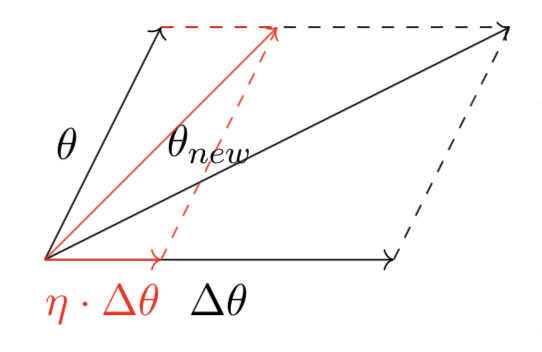
\includegraphics[width=10cm]{theta_vector}
\caption{\Large theta vector[\ref{OGD}]}
\label{theta_vector}
\end{center}
\end{figure}
\newpage
將$\theta$以泰勒展開式表示,假設並$\Delta\theta$為u:
\begin{center}
$L_{(\theta+\eta u)}=L_{(\theta)}+\eta u^{T}\cdot\bigtriangledown_{\theta} L_{(\theta)}+\frac{\eta^2}{2!}u^T\cdot\bigtriangledown^2 L_{(\theta)}u+\frac{\eta^3}{3!}...+\frac{\eta^4}{4!}...+\frac{\eta^n}{n!}...$\\
\end{center}
以泰勒展開式的型式表示的好處是:$\theta$些微的更動產生新值。$\eta$值通常小於一,當$\eta^2 << 1$,因此可以忽略高階項 
\begin{center}
$L_{(\theta+\eta u)}=L_{(\theta)}+\eta u^{T}\cdot\bigtriangledown_{\theta} L_{(\theta)} [\eta\ is\ typically\ small, so\ \eta^2, \eta^3,\cdots \rightarrow 0]$\\
\end{center}
新的$L(\theta + \eta u)$輸出的值會小於$L(\theta) L(\theta+\eta u) − L(\theta) < 0$,同理可證$u^T\cdot\bigtriangledown\theta L(\theta)$,符合u這條件:當新的值小於舊的值,u就是一個好的值。假設u和$\bigtriangledown\theta L(\theta)$的夾角為$\beta$\\
\begin{center}
$\cos(\beta)=\frac{u^{T}\cdot\bigtriangledown_{\theta} L_{(\theta)}}{\vert u^{T}\vert\vert \bigtriangledown_{\theta} L_{(\theta)}\vert}$\\
\end{center}
因為$\cos(\theta)$的值介於1和-1之間\\
\begin{center}
$-1<\cos(\beta)=\frac{u^{T}\cdot\bigtriangledown_{\theta} L_{(\theta)}}{\vert u^{T}\vert\vert \bigtriangledown_{\theta} L_{(\theta)}\vert}\leq 1$\\
$k=\vert u^{T}\vert\vert \bigtriangledown_{\theta} L_{(\theta)}\vert$\\
$-k \leq k\cos(\beta)=u^{T}\cdot\bigtriangledown_{\theta} L_{(\theta)}\leq k$
\end{center}
\newpage
 所以盡可能的讓新值小於舊值$(L(\theta+\eta u) − L(\theta) < 0)$,loss 值就會減少得越多。因此$u T \cdot \bigtriangledown\theta L(\theta)$應該為負,在這情況下$\cos(\beta)$於−1,$\beta$的角度為 $180^{\circ}$這就是$\theta$移動的方向與梯度方向相反的原因。 梯度下降法告訴我們:當$\theta$在特定值,並想減少新的$\theta$值,使 loss 值逐漸減少就應該與梯度相反的方向找 (若梯度為正值,找最小值就需往負的方向找):
\begin{center}
$w_{t=1}=w_t-\eta\bigtriangledown w_t$\\
$b_{t=1}=b_t-\eta\bigtriangledown b_t$\\
$where\ at\ w=w_t,b=b_t$\\
$\begin{cases}
 \bigtriangledown w_t=\frac{\partial L_{_{(\theta)}}}{\partial w}
 \bigtriangledown b_t=\frac{\partial L_{_{(\theta)}}}{\partial b}
 \end{cases}$
\end{center}
\item Batch gradient descrnt [\ref{OGD2}]\\
 Vanilla gradient descent 又稱 Batch gradient descent(批次梯度下降法),計算目標函數的梯度,參數$\theta$對於整個 訓練資料:
\begin{center}
$\theta=\theta-\eta\cdot\bigtriangledown_{\theta}L_{(\theta)}$
\end{center}
 目標函數以為例 loss function L($\theta$),參數$\theta$為 weight(w)和 bias(b)的函數,$\eta$為學習率。由於計算整個資料集計算梯度只更新一次,Bath gradient descent 可能非常慢並且對於資料集無法符合及記憶體來說棘手(一次需要儲存整個資料集的資料,當更新和計算時會占用大量記憶體)。\\
\begin{lstlisting}[caption=\Large Batch gradient descrnt]
 for i in range(nb_epochs) :
params_grad = evaluate_gradient (loss_function, data, params)
params = params − learning_rate * params_grad
\end{lstlisting}
\newpage
 預定義每次epoch,先計算loss function梯度向量對於整個資料集參數向量。如果梯度值來自於先前計算出的梯度值,就會檢查梯度,並以梯度相反的方向更新參數$\theta$,學習率$\eta$決定多大的更新量。Batch gradient descent對於凸面誤差可以保證收斂到廣域最小值,對於非面凸誤差可以收斂到局部最小值。
\item Stochastic gradient descent(SGD)[\ref{OGD2}]\\
隨機梯度下降法,這裡的目標函數為$J(\theta, x^i, y^i)$(變數$\theta$為 w(weight) 和 b(bias) 的函數,也可以寫成$J(w,b,\theta, x^i, y^i)$)。\\
\begin{center}
$\theta=\theta-\eta\cdot\bigtriangledown_{\theta}J_{(\theta, x^i, y^i)}$
\end{center}
批量梯度下降他會在每個參數更新前重新計算相似梯度。SGD 每次次執行會更新來消除多餘 (誤差),因此通常速度 很快。SGD 頻繁更新並變化很大,因為目標方程式波動很大(圖.\ref{sgd_fluctuation})。\\

\begin{figure}
\begin{center}
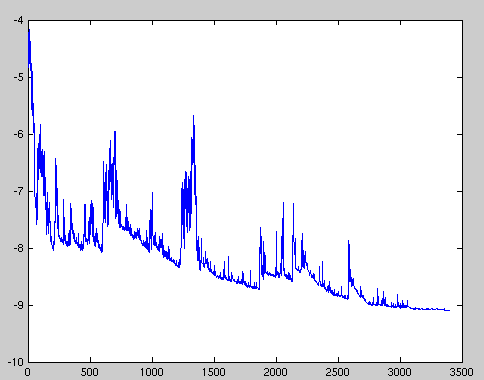
\includegraphics[width=10cm]{sgd_fluctuation}
\caption{\Large SGD fluctuation[\ref{OGD2}]}
\label{sgd_fluctuation}
\end{center}
\end{figure}
 SGD 的方程式一方面會跳到新的值和潛在局部最小值,另一方面 SGD 會持續超調 (誤差超過預期) 最後收斂到廣域最小值。無論如何他被顯示當學習率下降緩慢,SGD 顯示與 Batch gradient descent 同樣收斂行為,幾乎可以肯定地,對於凸面或非凸面優化,會收斂到絕對或是局部最小值。這程式碼片段[程式.2.2] 在訓練樣本上加入一個迴圈來對每個樣本評估梯度。每個 epoch(訓練循環) 會打亂訓練數據。
\label{code Stochastic gradient descrnt code}
\begin{lstlisting}[caption=\Large Stochastic gradient descrnt ]
for i in range(nb_epochs) :
np.random.shuffle(data)
for example in data :
params_grad = evaluate_gradient (loss_function, example, params)
params = params − learning_rate * params_grad
\end{lstlisting}
\item Mini-batch gradient descent[\ref{OGD2}]

 Mini-batch gradient descent(小批量梯度下降) 各取前兩者的優點,將資料集分割成小區塊,每個小區塊大小稱作 batch size,每次跑完 batch size 算迭代 (iteration)一次,算完一次資料集即完成一次 epoch。舉例: 資料集大小為1000,若 batch size 為50,iteration 為 datasets 的batch size  = 1000÷50 = 20,當 iteration 跑完 20 次算完成一次 epoch。\\
這方式可以減少參數更新的方差,並且可以穩定收斂;可利用深度學習庫所共有的高度優化的矩陣優化,從而由一個小批量計算出梯度非常有效。通常 batch sizes 的範圍介於 50 ~256,會因為應用而有所差異。訓練神經網絡時,通常選擇 Mini-batch gradient descent 算法,而當使用這算法時,通常也用 SGD 稱呼。\\
\begin{center}
$\theta=\theta-\eta\cdot\bigtriangledown_{\theta}J_{(\theta, x^{(i:i+n)}, y^{(i:i+n)})}$
\end{center}
下面[程式.2.3] 為迭代範例,batch size 大小為 50:\\
\label{Mini-batch gradient descrnt}
\begin{lstlisting}[caption=\Large Mini-batch gradient descrnt]
for i in range(nb_epochs ) :
np.random.shuffle(data)
for batch in get_batches (data, batch_size = 50):
params_grad = evaluate_gradient (loss_function, batch, params)
params = params − learning_rate ∗ params_grad
\end{lstlisting}
Mini-batch gradient descent 無論如何還是無法確保收斂的很好,存在一些需要解決的挑戰:
\begin{enumerate}[1]
\item 選擇適當的學習率是有難度的。如果學習率太小會導致收斂困難或緩慢,學習率太大則會阻礙收斂導致 loss function 來回波動或發生偏離。
\item 學習率清單嘗試在訓練的時候調整學習率,即根據預定義清單或當目標下降於閾值 (threshold) 時降低學習率。 但清單和閾值須預先定義,因此無法適應數據集的特徵。
\item 另外相同學習率適用全部參數更新。如果資料稀疏而且外型有很特別的頻率,我們可能不希望將所有特徵更新 到相同的程度,而是對很少發生的特徵執行較大的更新。
\item 最小化神經網路常見的高度非凸面誤差方程式 (error function) 的另一關鍵挑戰則是要避免被困在大量次優的局 部最小值區域中。認為困難實際上不是由局部最小值引起的,而是由鞍點引起的,即一維向上傾斜而另一維向下 傾斜的點。這些鞍點通常被相同誤差的平穩段包圍,這使得 SGD 很難逃脫,因為在所有維度上梯度都接近於零。
 \end{enumerate}
\item Gradient descent optimization algorithms[\ref{OGD2}]\\
SGD 難以在陡峭的往正確的方向,那就是說在一個維度上,曲面的彎曲比另一個維度要陡得多,這在局部最優情況下很常見。下圖(圖.1)的同心圓代表中心下凹的曲面。在這些情況下,SGD 會在陡峭的地方振盪,而僅沿著底部朝著局部最優方向猶豫前進,如(圖.\ref{fig.without_momentum}) 所 示。 Momentun(動量) 是一個幫助加速 SGD 在正確方向和抑制震盪的方法,在(圖.\ref{fig.with_momentum})。\\

\begin{figure}[hbt!]
\begin{center}
\subfigure{
\begin{minipage}[t]{0.5\linewidth}  %設定圖片間距

\includegraphics[width=6cm]{without}
\caption{\Large SGD without momentum[\ref{OGD2}]}
\label{fig.without_momentum}
\end{minipage}
}
\subfigure{
\begin{minipage}[t]{0.5\linewidth}

\includegraphics[width=6cm]{with}
\caption{\Large SGD with momentum[\ref{OGD2}]}
\label{fig.with_momentum}
\end{minipage}
}
\end{center}
\end{figure}

這麼做會增加一個係數$\gamma$來更新上次的向量到正確向量 (修正偏差),$\gamma$通常設為 0.9 左右。
\begin{center}
$v_t = \gamma v_{t-1}+\eta\cdot\bigtriangledown_{\theta}J_{(\theta)}$
$\theta = \theta-v_t$
\end{center}
 實際上,使用動量的時候,就像將球推下山坡。球在下坡時滾動時會累積動量,在途中速度會越來越快(如果存在空氣阻力,直到達到極限速度,也就是$\gamma < 1$) 參數更新也發生了同樣的事情:動量 (momentum) 對於梯度指向相同方向的維度增加,而對於梯度改變方向的維減少動量。結果,我們獲得了更快的收斂並減少了振盪。\\

 Nesterov accelerated gradient(NAG)是一種使動量具有一個去向的概念,以便在山坡再次變高之前知道它會減速。我們知道使用動量$\gamma v_{t-1}$來移動參數。計算$\theta - \gamma v_{t-1}$這樣就給了參數的下一個位置的近似值(完整更新缺少的梯度),這是參數將要存在的大致概念。現在,通過計算與當前參數無關的梯度來有效地看到目前的參數$theta$將會移動到的位置:
\begin{center}
$v_t = \gamma v_{t-1}+\eta\cdot\bigtriangledown_{\theta}J_{(\theta-\gamma v_{t-1})}$
$\theta = \theta - v_t$
\end{center}

\begin{figure}[hbt!]
\begin{center}
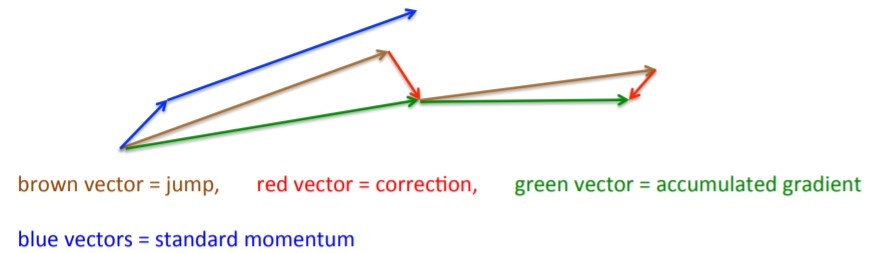
\includegraphics[width=13cm]{NAG}
\caption{\Large NAG[\ref{OGD2}]}
\label{NAG}
\end{center}
\end{figure}
同樣,我們設置動量$\gamma$約為0.9。動量首先計算當前梯度((圖.\ref{NAG})中的藍色小向量),然後在更新的累積梯度(藍 色向量)的方向上發生較大的跳躍,而 NAG 首先在先前的累積梯度的方向上進行較大的跳躍(棕色向量),測量梯度,然後進行校正(紅色向量),從而完成 NAG 更新(綠色向量)。這種預期的更新可防止我們過快地進行,並導致響應速度增加,從而顯著提高了 RNN 在許多任務上的性能。\\
Adagrad[\ref{OGD2}]:\\
 Adagrad 是一個梯度優化的算法,它可以做到:學習率適應參數,對於頻繁出現的特徵相關參數執行較小的更新(較低的學習率),以及對不經常出現的特徵相關參數進行較大更新(即學習率較高)。Adagrad可以提高SGD的強度,用於訓練大型神經網絡。\\
 先前,在同一次$theta$參數(更新後就算另一次),每個$theta$都使用相同的$\eta$(學習率)。Adagrad 則是對每個$theta$參數使用 不同的$\eta$,t 代表 time step。先將 Adagrad 的更新參數向量化。用$g_t$表示目標函數 (參數$theta$在 time step t) 對參數做偏微分計算。
\begin{center}
$g_{t,i}=\bigtriangledown_{\theta}J_{(\theta_{t,i})}$
\end{center}
當 SGD 更新每個參數$\theta_i$,在每個 time step t,因此變成:
\begin{center}
$\theta_{t+1,i}=\theta_{t,i}-\eta\cdot g_{t,i}$
\end{center}
更新規則,Adagrad 根據先前$\theta_i$計算的梯度,對每個參數$\theta_i$修改整個學習率$\eta$在每個 time stept:
\begin{center}
$\theta_{t+1,i}=\theta_{t,i}-\frac{\eta}{\sqrt{G_{t,ii}+\epsilon}}$
\end{center}
$G_t \in \mathbb{R}^{d\times d}$這是一個對角矩陣每個對角元素 i,i 是關於$theta$梯度平方和取決於 time stept,$\epsilon$是避免分母為0($\epsilon$通常為$10^{-8}$),如果沒有平方根運算,該算法的性能將大大降低。$G_t$包含了過去梯度平方根,由於全部$theta$參數沿著對角線,通過向量的內積計算$G_t$和$g_t$:
\begin{center}
$\theta_{t+1}=\theta_{t}-\frac{\eta}{\sqrt{G_{t}+\epsilon}}\cdot g_t$
\end{center}
 Adagrad 主要好處之一是,無需手動調整學習率。大多數實現使用預設值 0.01 並將其保留為預設值。Adagrad主要弱點是會累積分母的平方梯度:由於每項都是正的,累積和會在訓練中不斷增長。反過來,學習率下降,並最終變得無限小,這算法就不再獲得知識。\\
Adadelta[\ref{OGD2}]:\\
 Adadelta是Adagrad的延伸,下降其激進的程度,單調的降低學習率。Adadelta會限制過去累積的梯度,並將其限制在某個特定大小 w,並代替Adagrad過去累積的梯度平方,以梯度總和是遞迴定義為所有過去衰減梯度平方平均值。流動平均$E[g^2]_t$ 在time stept然後取決於(像Momentum的$\gamma$)先前平均和最近梯度:
\begin{center}
$E[g^2]_t=\gamma E[g^2]_{t-1}+(1-\gamma)g^2 _t$
\end{center}
$\gamma$值和 Momentum 的相似,約為 0.9,現在根據參數更新向量$\bigtriangleup\theta_t$來重寫 SGD:
\begin{center}
$\bigtriangleup\theta_t=-\eta\cdot g_{t,i}$\\
$\theta_{t+1}=\theta_t+\bigtriangleup\theta_t$
\end{center}
Adagrad 的參數更新向量替換成:對角矩陣$G_t$過去梯度平方的衰退平均$E[g^2]_t$
\begin{center}
$\bigtriangleup\theta_t=-\frac{\eta}{\sqrt{G_t+\epsilon}}\cdot g_t$\\
$replace\ G_t\ with\ E[g^2]_t\Rightarrow\bigtriangleup\theta_t=-\frac{\eta}{\sqrt{E[g^2]_t+\epsilon}}\cdot g_t$
\end{center}
由於分母只是梯度的均方根 (RMS),我們可以取代成縮寫:
\begin{center}
$\bigtriangleup\theta_t=-\frac{\eta}{RMS[g]_t}\cdot g_t$
\end{center}
 這個更新單位和 SGD、Momentum 以及 Adagrad 的單位不符合,因此更新需有相同的參數。為了實現這一點,首先定義另一個指數衰減平均值,這次不是梯度平方更新而是參數平方更新:
\begin{center}
$E[\bigtriangleup\theta^2]_t=\gamma E[\bigtriangleup\theta^2]_{t-1}+(1-\gamma)\bigtriangleup\theta^2 _t$
\end{center}
RMS 參數更新:
\begin{center}
$RMS[\bigtriangleup\theta]_t=\sqrt{E[\bigtriangleup\theta^2]_t+\epsilon}$
\end{center}
$RMS[\bigtriangleup\theta]_t$是未知的,更新參數的 RMS 取近似值到上個 time step。用$RMS[\bigtriangleup\theta]_t$取代學習率$\eta$,最後產生新的規則:
\begin{center}
$\bigtriangleup\theta_t=-\frac{RMS[\bigtriangleup\theta]_{t-1}}{RMS[g]_t}g_t$
\\
$\theta_{t+1}=\theta_t+\bigtriangleup\theta_t$
\end{center}
使用 Adadelta,甚至不需要設定預設學習率,因為它已從更新規則淘汰。\\
RMSprop[\ref{OGD2}]:\\
 RMSprop 是 Geoffrey Hinton 在他的課程中提出的未公開自適應學習率的方法。\\

 RMSprop 和 Adadelta 都是為了解決 Adagrad 的學習率急劇下降的問題個別獨立開發出來的解決方式。RMSprop 實際上與 Adadelta 得出的第一個更新向量相同:
\begin{center}
$E[g^2]_t=0.9E[g^2]_t+0.1g^2 _t$
\\
$\theta_{t+1}=\theta_t-\frac{\eta}{\sqrt{E[g^2]_t+\epsilon}}g_t$
\end{center}

 RMSprop 也將學習率除以梯度平方的指數衰減平均值。Hinton 建議$\gamma$設為 0.9,好的預設學習率$\gamma$數值為 0.001。\\
Adaptive Moment Estimation:[\ref{OGD2}]\\
 Adaptive Moment Estimation 自適應矩評估 (Adam) 是另一種計算每個評估學習率的方法。出了儲存過去梯度平 方的指數衰減平均值$v_t$,就像 Adadelta 和 RMSprop 一樣,Adam 還保留過去梯度的指數衰減平均值$m_t$,類似動量 (Momentum)。如果 Momentum 被視為順著斜坡下滑的球,而 Adam 則是像一個帶有摩擦的沉重的球,因此更適合待在 error face 平坦的最小值區域。計算過去梯度平方的衰減平均值$m_t$和$v_t$分別如下:
\begin{center}
$m_t=\beta_1 m_{t-1}+(1-\beta_1)g_t$\\
$v_t=\beta_2 v_{t-1}+(1-\beta_2)g^2 _t$
\end{center}
$m_t$和$v_t$分別是第一階矩平均估計值和第二階矩無中心方差估計值,因此是方法的名稱。像$m_t$和$v_t$被初始化為向量 o,Adam 的作者觀察到它們偏向零,特別是在初始 time step,尤其是在衰減率較小的時候 (也就是說$\beta_1$和$\beta_2$趨近於 1) 藉由計算校正偏差第一矩$\hat{m}_t$和第二矩$\hat{v}_t$抵消偏差:
\begin{center}
$\hat{m}_t = \dfrac{m_t}{1 - \beta^t_1}$\\
$\hat{v}_t = \dfrac{v_t}{1 - \beta^t_2}$
\end{center}
使用他們去更新參數,就像 Adadelta 和 RMSprop 中所看到的那樣,這將產生 Adam 更新規則:
\begin{center}
$\theta_{t+1} = \theta_{t} - \dfrac{\eta}{\sqrt{\hat{v}_t} + \epsilon} \hat{m}_t$
\end{center}
$\beta_1$預設值建議為 0.9,$\beta_2$預設值建議為 0.999,ϵ 預設值建議為$10^{-8}$。根據經驗證明 Adam 表現良好,並且與其他自適應學習算法相比具有優勢。
在 Adam 更新規則中的$v_t$係數是與梯度成反比地縮放過去梯度的範數 (通過 $v_{t-1}$項) 和當前梯度$|g_t|^2$:
\begin{center}
$v_t = \beta_2 v_{t-1} + (1 - \beta_2) |g_t|^2$
\end{center}
我們轉換這個更新到$\ell_p$。注意$\beta_2$參數化為$\beta_2^p$:
\begin{center}
$v_t = \beta_2^p v_{t-1} + (1 - \beta_2^p) |g_t|^p$
\end{center}
大規範 p 值使數值上變得不穩定,這就是為什麼$\ell_1$和$\ell_2$規範在實踐中是最常見的。然而$\ell_\infty$通常也表現出穩定 的行為。為了避免與 Adam 混用,所以使用$u_t$來表示無窮範數約束$v_t$:
\begin{center}
$u_t = \beta_2^\infty v_{t-1} + (1 - \beta_2^\infty) |g_t|^\infty$\\
$= \max(\beta_2 \cdot v_{t-1}, |g_t|)$
\end{center}
替換為Adam更新公式$\sqrt{\hat{v}_t} + \epsilon$和$u_t$得出AdaMax更新規則:
\begin{center}
$\theta_{t+1} = \theta_{t} - \dfrac{\eta}{u_t} \hat{m}_t$
\end{center}
替換為Adam更新公式$\sqrt{\hat{v}_t} + \epsilon$和$u_t$得出AdaMax更新規則:
\begin{center}
$\theta_{t+1} = \theta_{t} - \dfrac{\eta}{u_t} \hat{m}_t$
\end{center}
注意$u_t$依靠最大運算,不建議 Adam 中的$m_t$和$v_t$偏向零,這就是為什麼不需要針對$u_t$計算偏差。好的預設值$\eta = 0.002$ $\beta_1 = 0.9$ 和 $\beta_2 = 0.999$。\\
\end{itemize}


\section{強化學習}
%=----------What is Reinforcement Learning?------------=%
強化學習(Reinforcement Learning,簡稱為RL)是通過agent(代理)與已知或未知的環境持續互動,不斷適應與學習,會得到正向或負面的回饋,對應到獎賞(reward)和懲罰(punishments)。考慮到agent與環境(environment)互動,進而決定要執行哪個動作,強化學習的學習模式是建立在獎賞與懲罰上。\\

強化學習與其他學習法不一樣的地方在於:不需要事先收集大量數據提供當作學習樣本,而是透過與環境互動,在環境下發生的狀態當作學習的資料來源,透過不斷嘗試使所得到的獎勵最大化。其他類型的機器學習大都需要給予特定資料且有明確的答案。\\

由於強化學習是建立在agent與環境互動上,因此許多參數進行運算,需要大量資訊來學習,並根據資訊採取行動。強化學習的環境可以是真實世界、2D或3D模擬世界的場景。強化學習的範圍很廣,因為環境的規模可能很大,且在環境中有多相關因素,影響著彼此。強化學習以獎勵的方式,促使學習結果趨近或達到目標結果。\\
%=----------Faces of Reinforcement Learning---------------=%

強化學習涵蓋範圍(圖.\ref{各領域與機器學習應用範圍}):\\
 強化學習可以運用在計算機科學、神經科學、心理學、經濟學、數學、工程等領域,涵蓋領域相當廣泛。
%======需文字補充========%
\begin{figure}[hbt!]
\begin{center}
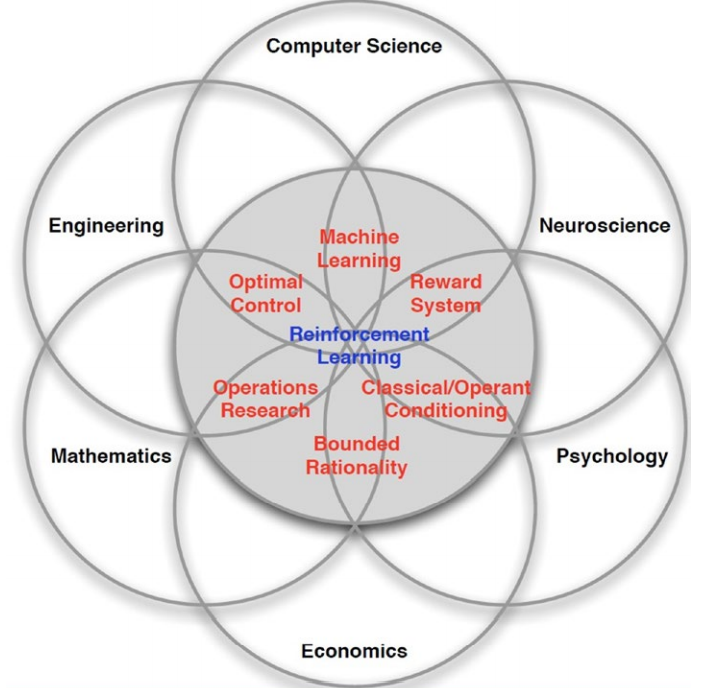
\includegraphics[width=11cm]{Faces_of_Reinforcement_Learning}
\caption{\Large 各領域與機器學習應用範圍}
\label{各領域與機器學習應用範圍}
\end{center}
\end{figure}
%=--------The Flow of Reinforcement Learning------------=%.
\newpage
強化學習的流程:\\
透過agent與環境間互動而產生狀態和獎勵,由於狀態的轉移,agent會決定接下來執行動作(圖.\ref{RL structur})。\\[12pt]

\begin{figure}[hbt!]
\begin{center}
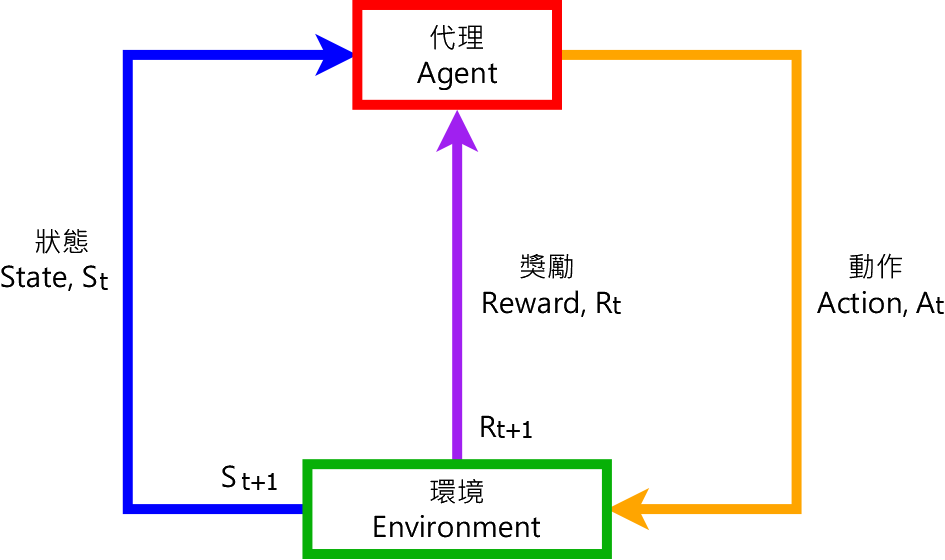
\includegraphics[width=12cm]{The_Flow_of_Reinforcement_Learning}
\caption{\Large 強化學習架構}
\label{RL structur}
\end{center}
\end{figure}
需要考慮的重點:\\
強化學習的狀態、獎勵和動作是互相關聯,agent與環境之間存在著關聯,兩者都影響著狀態和動作並互相影響著彼此:機器人會因動作而造成狀態轉移,狀態的移轉也會影響機器人做出的決策。\\
\newpage
\begin{figure}[hbt!]
\begin{center}
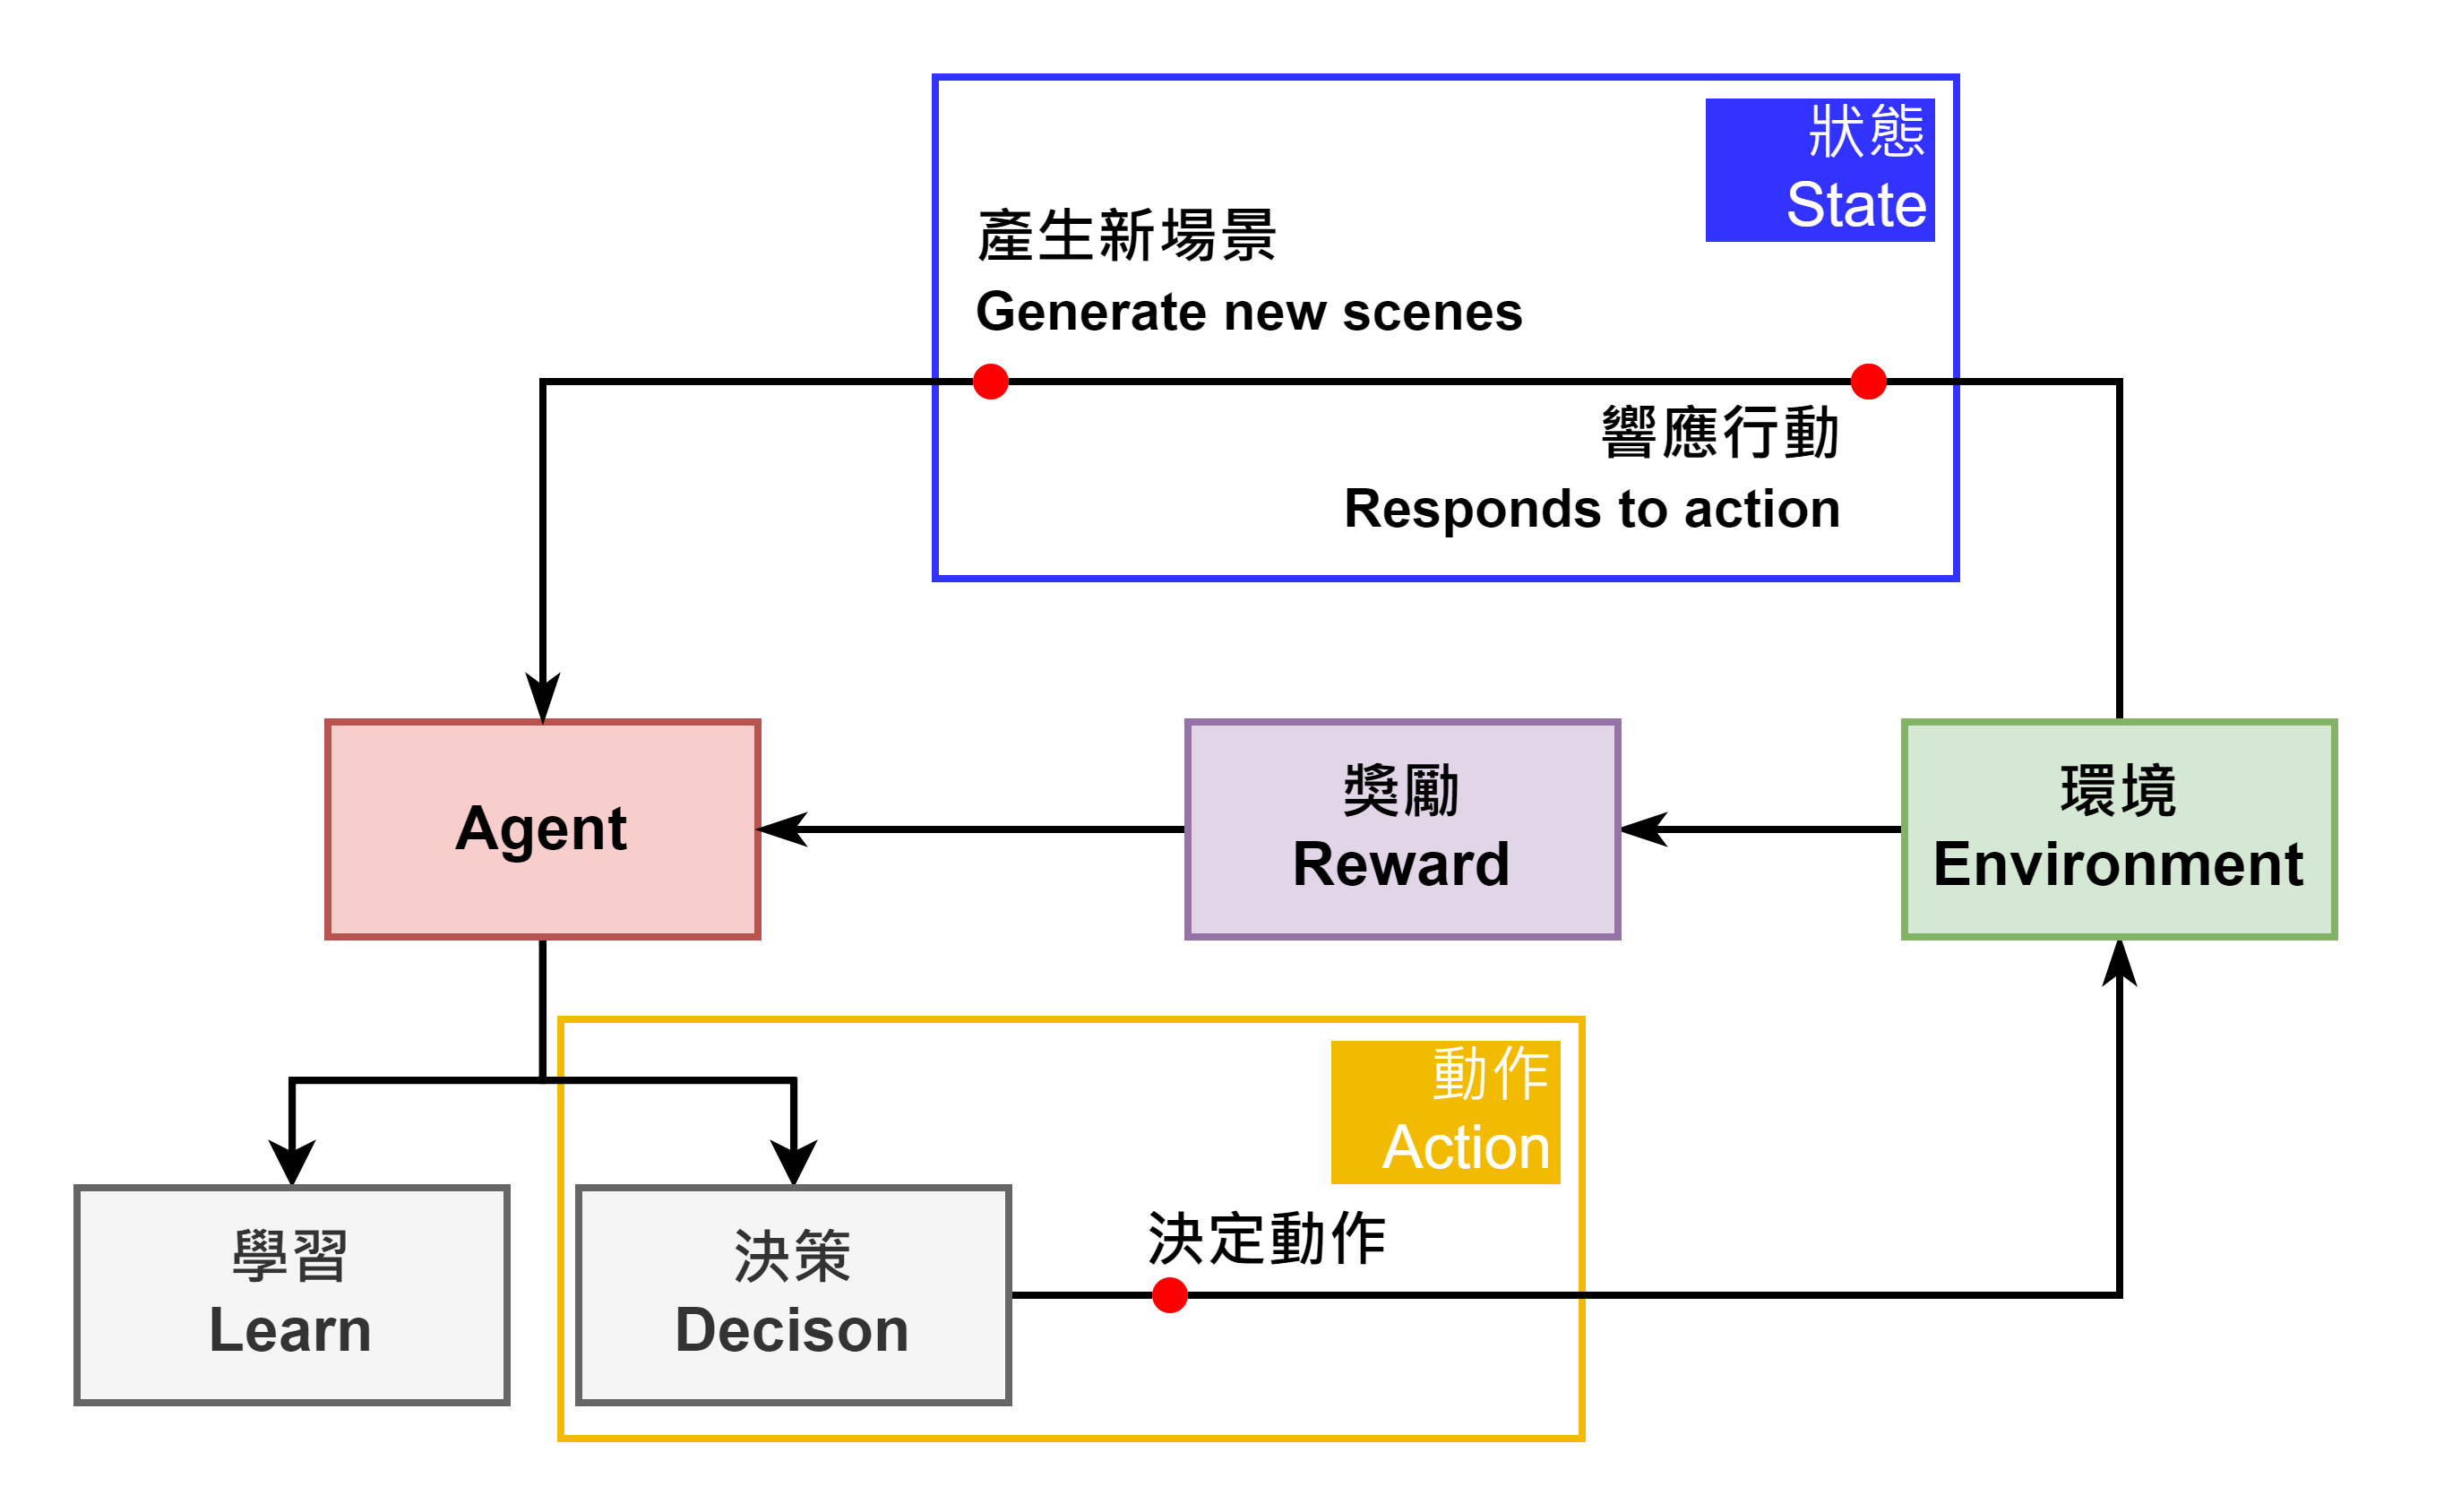
\includegraphics[width=15cm]{The_entire_interaction_process}
\caption{\Large 整個互動過程}
\label{整個互動過程}
\end{center}
\end{figure}
 如(圖.\ref{整個互動過程}) agent會透過輸入的狀態來決定採取何種行為(動作),並試圖採取獲得最高獎勵的行動。當agent開始與環境互動時,agent會透過當前狀態來決定將採取的行動,在agent採取行動後,環境的狀態也因此而改變,若agent採取行動後所到達我們所要的狀態就會得到獎勵,反之則會給予懲罰。在場景裡透過反覆的訓練,讓強化學習的行為漸漸趨近預期的目標。\\
%=----Different Terms in Reinforcement Learning----------=%
 強化學習中有兩個很重要的常數:$\gamma$和$\lambda$。\\
 
$\gamma$會影響所獲得的獎勵。$\gamma$又稱為衰減因子,正常狀態下為小於1的常數用於每個狀態改變,當狀態改變時為時常數。$\gamma$允許使用者在每個狀態給予不同形式的獎勵(這種狀況下$\gamma$為0),如果著重在長期的決策時,獎勵就不受決策順序所影響(此時$\gamma$為1)\\

$\lambda$一般在我們處理時間差異問題時使用。 這是涉及更多地連續狀態的預測。在每個狀態中$\lambda$值的增加代表演算法正在快速學習。\\
%------------------圖片可共用----------------------%
\iffalse
\begin{figure}[hbt!]
\begin{center}
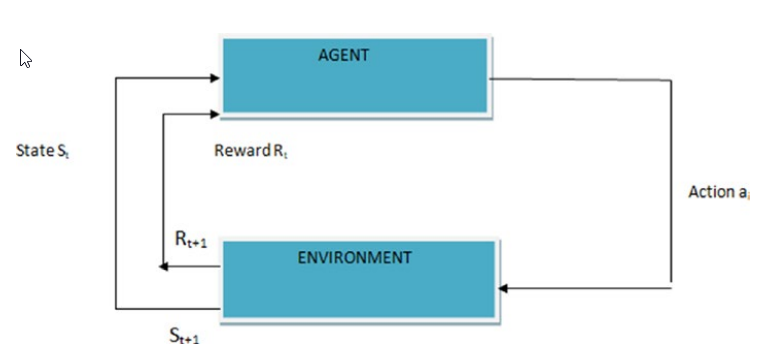
\includegraphics[scale=0.74]{ Reinforcement_Learning_interactions}
\caption{\Large Reinforcement Learning interactions}
\end{center}
\end{figure}
\fi
%=----Interactions with Reinforcement Learning------------=%

強化學習的互動是透過agent和環境之間的互動會產生獎勵,agent採取行動,導致狀態改變是一種強化學習實現如何將情況映設為行動的方法,從而找到最大化獎勵的方法,機器或機器人不會像其他機器學習形式的機器人那樣被告知要採取哪些行動。\\

獎勵的目的與運作以獎勵的方式誘導機器採取我們所期望的動作,機器會採取最大化獎勵的方式,因此可將目的定為最大獎勵,以吸引機器執行期望做的行為。\\

\begin{figure}[hbt!]
\begin{center}
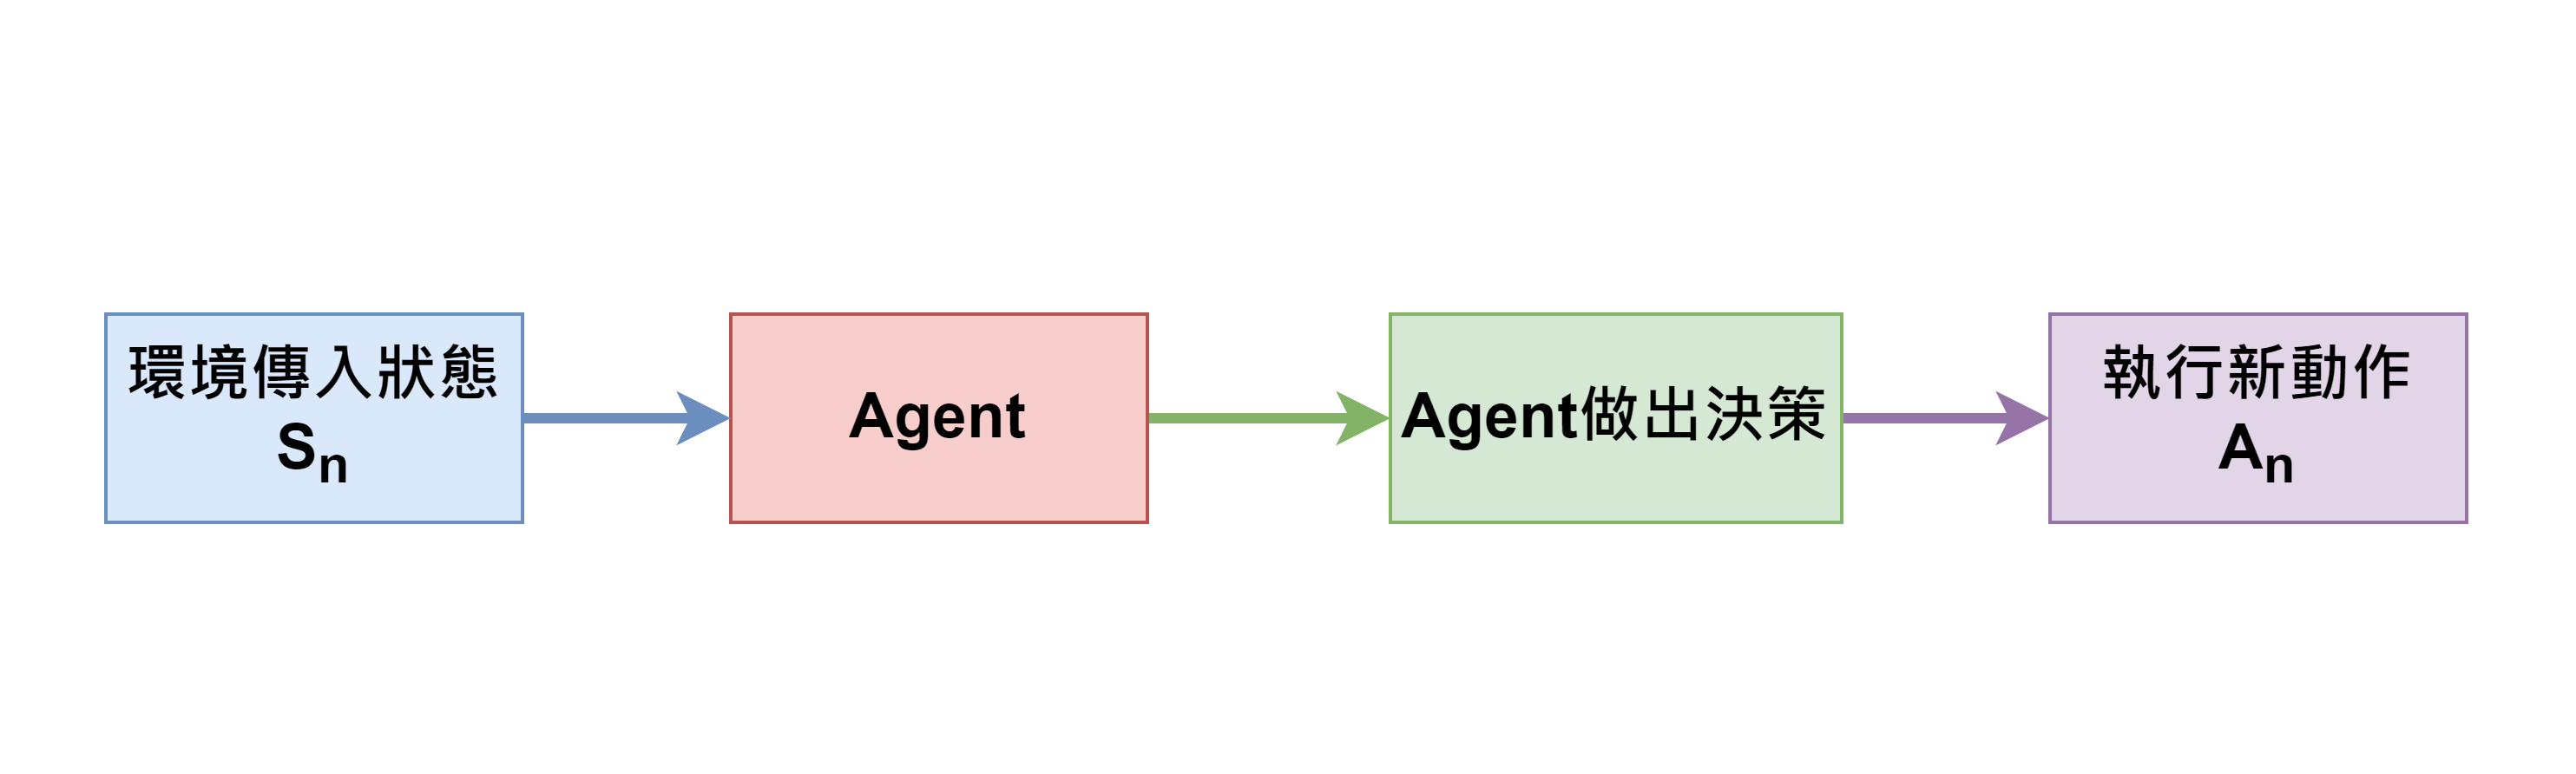
\includegraphics[width=15cm]{agent}
\caption{\Large agent}
\label{agent}
\end{center}
\end{figure}
%=----Agents------------=%
\begin{flushleft}
強化學習的環境:\\
\end{flushleft}
強化學習中的環境由某些因素組成,會對agent產生影響,agent必須根據環境適應各種因素,並做出最佳決策,這些環境可以是各種形式,其中包括2D、3D或是真實世界。強化學習的環境具有確定性、可觀察性,可以是離散或是連續的狀態,則agent可以是單一或多個所組成。\\
\subsection{馬可夫決策}
\begin{itemize}
\item Markov Chain\\
 馬可夫鏈(Markov Chain)主要是狀態變化的隨機過程(stochastic process)和馬可夫屬性(Markov property)結合。隨機過程(stochastic process)狀態隨著時間變化,而狀態的變化存在著雖機性,並以數學模式表示。馬可夫屬性(Markov property)指在目前以及所有過去事件的條件下,任何未來事件發生的機率,和過去的事件不相關僅和目前狀態相關。當前決策只會影響下個狀態,當前狀態轉移(action)到其他狀態的機率會有所差異。\\
\item Markov Reward Process\\
\begin{itemize}
\item action 到指定狀態會獲得獎勵。
$$R(s_t=s) = \mathbb{E}[r_t|s_t = s]$$
$$\gamma \in [0, 1]$$
\item Horizon:
在無限的狀態以有限的狀態表示。
\item Return:
越早做出正確決策獎勵越高。
$$G_t = R_{t+1}+\gamma R_{t+2}+\gamma^2 R_{t+3}+\gamma^3 R_{t+4}+...+\gamma^{T-t-1} R_{T}$$
\item State value function(決策價值):
$$V_t(S) = \mathbb{E}[G_t|s_t = s]$$
$$P(s_{s+1}=s'|s_t=s,a_t=a)$$
\end{itemize}
\item Discount Factor ($\gamma$)
獎勵衰減有幾種作法:第一種,越早做出有獎勵的決策,獎勵越高:第二種,做出有價值的決策$\gamma = 1$,不分決策順序先後;第三種,無用的決策$\gamma = 0$,不會得到獎勵。\\
以Bellman equation的方式描述互動關係狀態:\\
$$V(s) = R(s)+\gamma\sum_{s'\in S}P(s'|s)V(s')$$
\begin{center}
$R(s)$:立即獎勵\\
$\gamma\sum_{s'\in S}P(s'|s)V(s')$:未來獎勵衰減總和
\end{center}
Anaytic solution(分析性解法),MRP的分析性解法:
$$V = (1-\gamma P)^{-1}R$$
Bellman equation及Anaytic solution的方式只適合小的MRP(個數比較少的),矩陣複雜度為$O(N^3)$,N為狀態個數。若要計算大型的MRP會使用疊代法:動態規劃(Dynamic programming)、Temporal-Difference learning和Mote-Carlo evaluation以評估採樣的方式:
$$g = \sum_{i=t}^{H-1}\gamma^{1-t}r_i$$
$$G_t \leftarrow G_t+g,  i \leftarrow i+1$$
$$V_t(s) \leftarrow \frac{G_t}{N}$$
\item Markov Decision Process在MRP中加入決策(decision)和動作(action)
\begin{itemize}
\item S:state 狀態
\item A:action 動作
\item P:狀態轉換
$P(s_{s+1}=s'|s_t=s,a_t=a)$
\item R:獎勵,取決於當前狀態和動作會得到相對應的講勵
$$R(s_t=s, a_t=a) = \mathbb{E}[r_t|s_t, a_t=a]$$
\item D:折扣因子(discount factor)
$$\gamma \in [0,1]$$
\end{itemize}
\end{itemize}

\begin{flushleft}
policy(決策):可以是一個決策行為的機率或確定執行的行為,若以數學方程式表示:
$$\pi (a|s) = P(a_t=a|s_t=s)$$
\newpage

MRP和MDP方程式互相轉換:\\
\end{flushleft}
%=========表格=========%
\begin{center}
\begin{tabular}[c]{ccc}    
%\multicolumn{1}{r}{MRP}
 MRP & $\longleftrightarrow$ & MDP\\
\hline
$P^{\pi}(s's)$ & = & $\sum_{a\in A}\pi (a|s)P(s'|s, a)$\\
$P^{\pi}(s)$ & = & $\sum_{a\in A}\pi (a|s)P(s, a)$\\
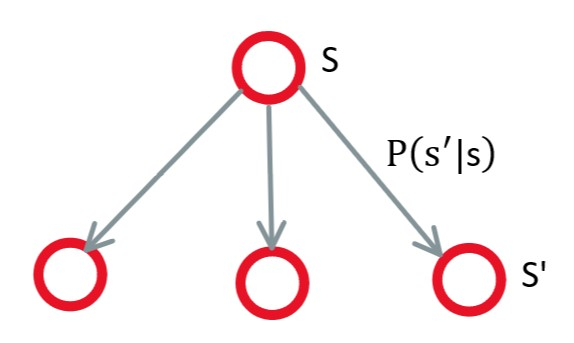
\includegraphics[height=3cm]{MRP}&&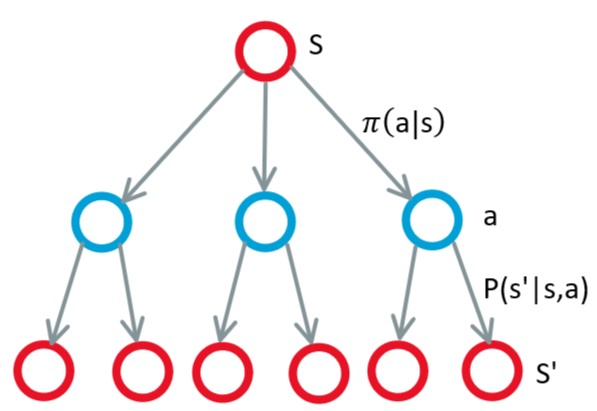
\includegraphics[height=3cm]{MDP}\\
\hline
\end{tabular}
\end{center}
\hspace{15pt}
 
state value function(狀態值方程式)$v^{\pi}(s)$\\
$$v^{\pi}(s) = \mathbb{E}[G_t|s_t=s]$$
$$= \mathbb{E}[R_{t+1}+\gamma v^{\pi}(s_{t+1})|s_t=s]$$
$$= \sum_{a\in A}\pi (a|s)q^{\pi}(s, a)$$
\begin{figure}[hbt!]
\begin{center}
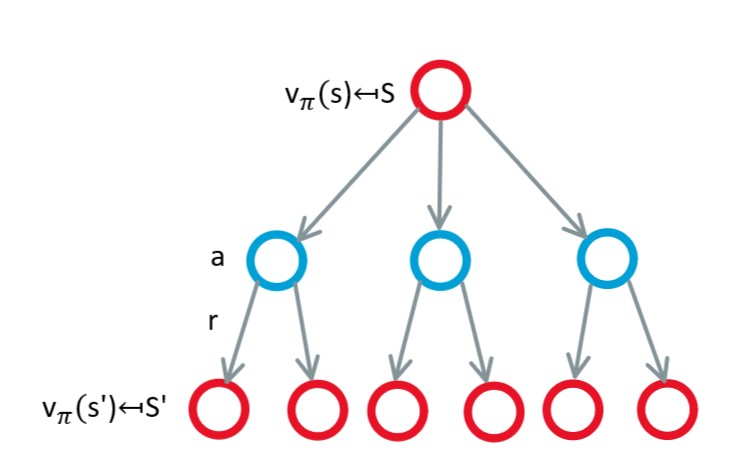
\includegraphics[width=8cm]{s_to _s}
\caption{$v^{\pi}$程序圖}
\label{fig.s_to_s}
\end{center}
\end{figure}
$$v^{\pi}(s) = \sum_{a\in A}\pi (a|s)(R(s, a)+\gamma \sum_{s'\in s}P(s'|s, a)v^{\pi}(s'))$$
\newpage
state value function(狀態值方程式)$q^{\pi}(s)$
$$v^{\pi}(s) = \mathbb{E}[G_t|s_t=s]$$
$$= \mathbb{E}[R_{t+1}+\gamma v^{\pi}(s_{t+1})|s_t=s]$$
$$= \sum_{a\in A}\pi (a|s)q^{\pi}(s, a)$$
\begin{figure}[hbt!]
\begin{center}
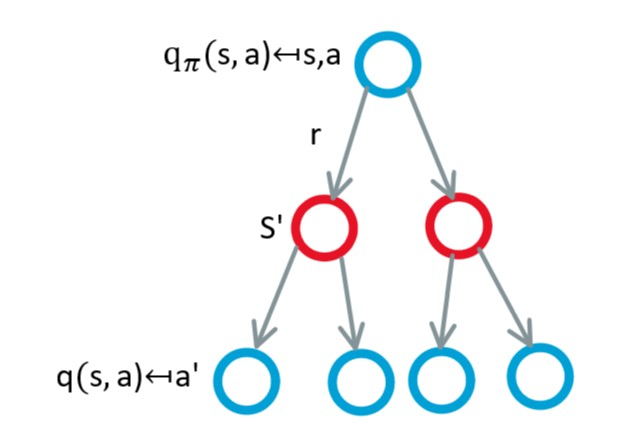
\includegraphics[width=8cm]{Q_pi function}
\caption{$q^{\pi}$程序圖}
\label{fig.q_pi}
\end{center}
\end{figure}
$$q^\pi(s, a)=R(s, a)+\gamma\sum_{s'\in S}P(s'|s, a)\sum_{a'\in A}\pi(a'|s')q^{\pi}(s', a')$$
\newpage
\section{Policy Gradient理論}
\begin{figure}[hbt!]
\begin{center}
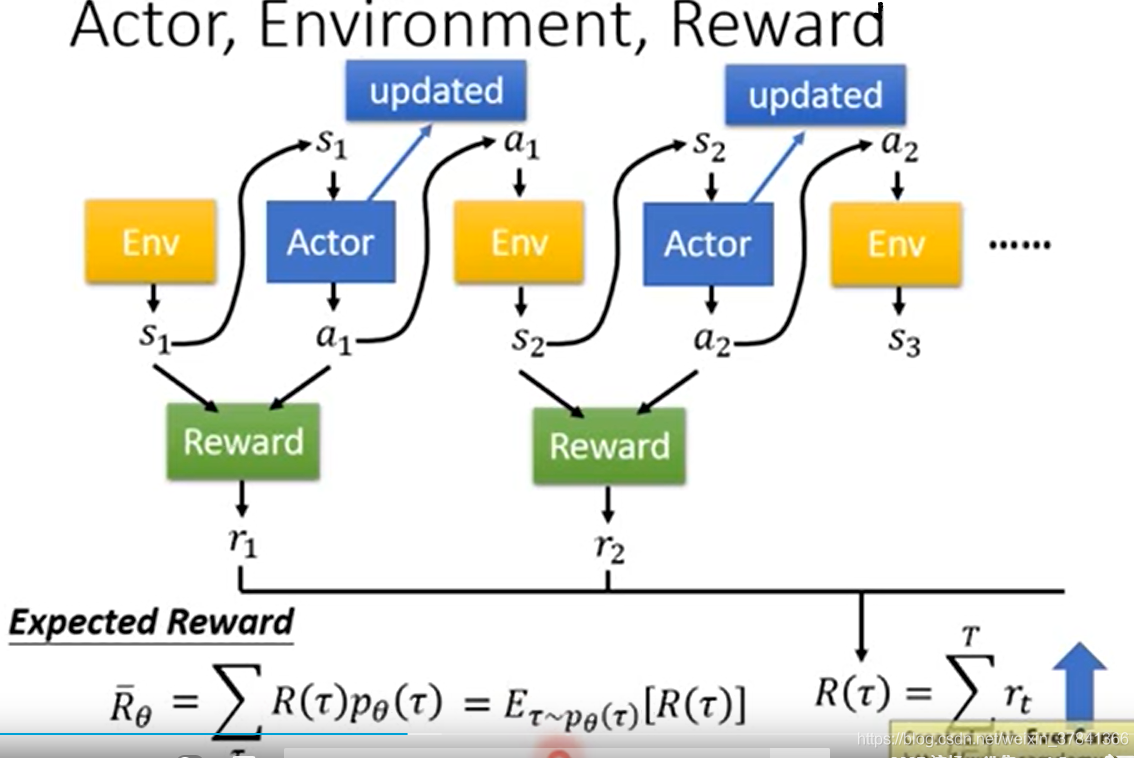
\includegraphics[width=15cm]{policy gradient原理}
\caption{\Large Policy Gradient原理}
\label{Policy Gradient原理}
\end{center}
\end{figure}

Policy Gradient主要目的是直接對決策進行建模與優化。該決策(policy)通常使用參數化函數建模,獎勵(目標)函數的值取決於此決策,可以應用各種算法來優化,以獲得最佳獎勵。(參數化:當軟體建置於一給定環境時,再依該環境的實際需求填選參數,即可成為適合該環境。)\\
參數介紹[\ref{R.Policy Gradient}]:\\
$\pi$:policy\\
s:狀態(States)。\\
a:動作(Actions)。\\
r:獎勵(Rewards)。\\
$S_t,A_t,R_t$:一個軌跡時間步長't'的State,Action and Reward。 \\
$\gamma$:衰減因子(Discount Factor);懲罰未來的不確定獎勵(reward)。\\
$G_t$:回傳衰減後的未來獎勵(Discounted future reward)$G_t = \sum_{k=0}^{\infty} \gamma^k R_{t+k+1}$\\
$P(s', r \vert s, a)$:伴隨著現在狀態(state)的a和r,前往下一個狀態s'的轉移機率矩陣(單階)。\\
$\pi(a \vert s)$:隨機策略(agent的行為策略)。\\
$\mu(s)$:確定的策略;我們還使用不同的字母將其標記為$ \pi(s)$,以提供更好的區分,以便我們可以輕鬆判斷策略是隨機的還是具有確定性的\\
$V(s)$:'狀態值函數'測量狀態的預期收益(報酬率)\\
$V^\pi(s)$:根據policy的狀態值函數$V^\pi (s) = \mathbb{E}_{a\sim \pi} [G_t \vert S_t = s]$\\
$Q(s, a)$:行為值函數,評估一對狀態和動作的預期收益。\\
$Q^\pi(s, a)$:根據policy的行為值函數$Q^\pi(s, a) = \mathbb{E}_{a\sim \pi} [G_t \vert S_t = s, A_t = a]$。\\
$A(s, a)$:Advantage Function,$A(s, a) = Q(s, a) - V(s)$:像是另一種版本的Q-value,由狀態值為基準降低方差。\\
reward function的值:取決於策略,可應用各種算法優化$\theta$,獲得最佳獎勵。\\[5pt]
$$J(\theta) 
= \sum_{s \in \mathcal{S}} d^\pi(s) V^\pi(s) 
= \sum_{s \in \mathcal{S}} d^\pi(s) \sum_{a \in \mathcal{A}} \pi_\theta(a \vert s) Q^\pi(s, a)$$\\

Policy Gradient 通過反覆評估梯度來最大化預期的總獎勵(reward)\\[5pt]
$g = \nabla_\theta\mathbb{E}[\sum_{t=0}^\infty r_t]$ ; $g = \mathbb{E}[\sum_{t=0}^\infty\psi_t\nabla_\theta log\pi_\theta(a_t \vert s_t)]$\\[5pt]
\begin{Large}{$\psi_t$ 可能方法為下列:}\end{Large}
\begin{itemize}
\item $\sum_{t=0}^\infty r$:決策軌跡的獎勵總和。
\item $\sum_{t^{'}=t}^\infty r^{'}$: 根據動作(action)的獎勵(reward) $a_t$。\\
標準表示式:$\sum_{t^{'}=t}^\infty r_t^{'}-b(s_t)$
\item $Q^\pi(s_t,a_t)$:state-action value function。
\item $A^\pi(s_t,a_t)$:Advantage Function。
\item $r_t+V^\pi(s_t+1)-V^\pi(s_t)$:TD residual。
\end{itemize}
公式使用定義[\ref{R.Policy Gradient}]:\\[5pt]
$V^\pi(s_t) = \mathbb{E}_{s_{t}+1:\infty,a_{t}:\infty}[\sum_{l=0}^\infty r_t+l]$\\[5pt]
$Q^\pi(s_t,a_t) = \mathbb{E}_{s_{t}+1:\infty_,a_{t}+1:\infty}[\sum_{l=0}^\infty r_t+l]$\\[5pt]
$A^\pi(s_t,a_t) = Q^\pi(s_t,a_t)-V^\pi(s_t)(Advantage Function)$\\[5pt]

\subsection{Actor Critic}
原始的policy gradient沒有偏差,但方差大;所以提出了許多以下算法來減少方差,同時保持偏差不變:\\[5pt]
$$g = \mathbb{E}[\sum_{t=0}^\infty\psi_t\nabla_\theta log\pi_\theta(a_t \vert s_t)]$$\\[5pt]
Actor-Critic:減少原始政策中的梯度方差包括兩個模型\\[5pt]
Critic:更新值函數參數w,根據算法,它可以是操作值$ Q_w$($a \vert s$)或狀態值$V_w$($s$) \\[5pt]
Actor:按照Critic的建議,將策略參數 $\theta$ 更新為 $\pi_\theta$($a \vert s$)\\[5pt]
\begin{Large}
它如何在簡單的行動價值參與者批評中發揮作用:
\end{Large}
\begin{itemize}
\item 隨機的初始化 s,$\theta$,w ;取樣 a $\sim
\pi_\theta(a \vert s)$
\end{itemize}
\begin{itemize}
\item For $t =1 \sim T:$ 
\begin{enumerate}[1]
\item 取樣 reward $r_t$ $\sim$ $R(s,a)$ 隨後下一階段 $s'$ $\sim$ $P(s'\vert s,a)$ 
\item 樣本的下一個動作 $a' \sim$ $\pi_\theta(a'\vert s')$
\item 更新 policy 參數 $\theta$ :\\
$$\theta\leftarrow\theta+\alpha_\theta Q_w(s,a)\nabla_\theta ln\pi_\theta(a\vert s)$$
\item 計算校正 (TD error)對於時間t的動作值:\\
$$\delta = r_t + \gamma Q_w(s',a')-Q_w(s,a)$$
並使用它來更新操作action - value function:\\
$$w\leftarrow w+\alpha_w \delta \nabla_w Q_w(s,a) $$
\item 更新 $a\leftarrow a'$ 和 $ s \leftarrow s'$ ; 學習率:$a_\theta$ 和 $a_w$。
\end{enumerate}   
\end{itemize}\newpage

\iffalse
\subsection{Policy Gradient Theorem}
Policy Gradient 通過反覆估計梯度來最大化預期的總reward\\[5pt]
$g = \nabla_\theta\mathbb{E}[\sum_{t=0}^\infty r_t]$ ; $g = \mathbb{E}[\sum_{t=0}^\infty\psi_t\nabla_\theta log\pi_\theta(a_t \vert s_t)]$\\[5pt]
\begin{Large}{$\psi_t$ 可能方法為下列:}\end{Large}
\begin{itemize}
\item $\sum_{t=0}^\infty r$:決策軌跡的獎勵總和。
\item $\sum_{t^{'}=t}^\infty r^{'}$: 根據動作(action)的獎勵(reward) $a_t$。\\
標準表示式:$\sum_{t^{'}=t}^\infty r_t^{'}-b(s_t)$
\item $Q^\pi(s_t,a_t)$:state-action value function。
\item $A^\pi(s_t,a_t)$:Advantage Function。
\item $r_t+V^\pi(s_t+1)-V^\pi(s_t)$:TD residual。
\end{itemize}
公式使用定義:\\[5pt]
$V^\pi(s_t) = \mathbb{E}_{s_{t}+1:\infty,a_{t}:\infty}[\sum_{l=0}^\infty r_t+l]$\\[5pt]
$Q^\pi(s_t,a_t) = \mathbb{E}_{s_{t}+1:\infty_,a_{t}+1:\infty}[\sum_{l=0}^\infty r_t+l]$\\[5pt]
$A^\pi(s_t,a_t) = Q^\pi(s_t,a_t)-V^\pi(s_t)(Advantage Function)$\\[5pt]
\section{類神經網路中強化學習的應用}
\begin{figure}[hbt!]
\begin{center}
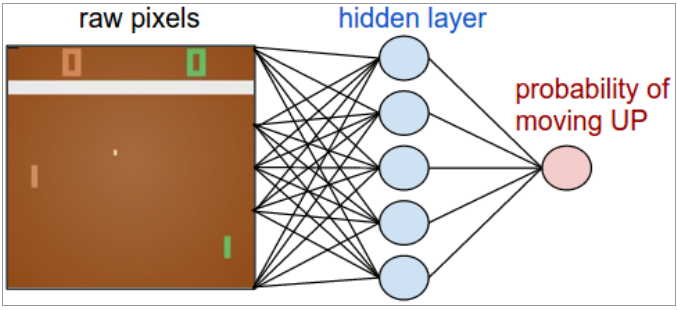
\includegraphics[scale=0.74]{network}
\caption{實際兩層神經網路}
\end{center}
\end{figure}

 我們將定義一個可以執行玩家(agent)的類神經網路,該網路將獲取遊戲狀態並決定我們應該做什麼(向上移動或向下移動我們使用一個2層神經網路,該網路獲取原始圖像像素(100,800個數字(210*160*3)),並生成一個表示上升概率的數字。 使用隨機策略是標準做法,這意味著我們只會產生向上移動的可能性,每次迭代時,我們都會從該分布中採樣(即扔一枚有偏見的硬幣)已獲得實際移動。\\

\subsection{監督式學習}
\begin{figure}[hbt!]
\begin{center}
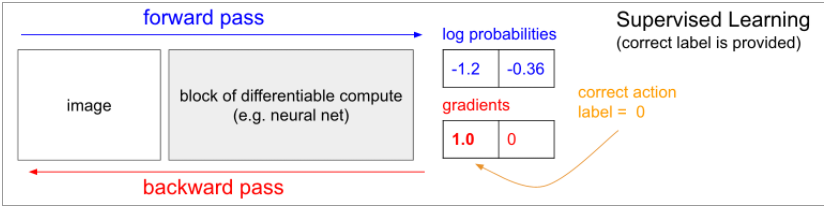
\includegraphics[scale=0.74]{supervising_learning}
\caption{監督式學習}
\end{center}
\end{figure}

 在我們深入探討 Score Function 解決方案之前,需要簡短介紹有關監督學習的知識,因為正如看到的,與我們架構類似,在普通的監督學習中,我們會將圖像傳送到網路,並獲得一概率值,例如對於兩個類別的上和下。 這裡顯示的是向上和向下對數概率(-1.2,-0.36),而不是原始機率(在這個情況下,是30$\%$和70$\%$),因為我們總是優化正確標籤的對數概率(這使我們的演算法更好,並等效於優化原始概率,因為對數是單調的),而在監督學習中,我們將可以獲取標籤,例如:
我們可能被告知現在正確的做法是向上運動(標籤0),在執行過程中,我們將以上的對數機率輸入1.0的梯度,然後運行反向傳播來計算梯度向量$Wlogp(y=UP|x)$這個梯度將告訴我們應如何更改百萬個參數中的每個參數,使網路預測往上的可能性更高,例如:網路中的百萬個參數之一可能具有-2.1的梯度,這意味著如果我們將該參數增加一個小的正值(例如0.001),則往上的對數機率將因2.1*0.001而降低(由於負號而減少),如果我們隨後更新了參數,當之後遇到非常相似的圖像時(也就是環境狀況),我們的網路現在更有可能預測往上。\\

\subsection{對數導數技巧}
 機器學習涉及操縱機率。這個機率通常包含歸一化概率或對數概率。能加強解決現代機器學習問題的關鍵點,是能夠巧妙的在這兩種型式間交替使用,而對數導數技巧就能夠幫助我們做到這點,也就是運用對數導數的性質。\\
 
\subsection{為什麼選擇score function 算法}
 多篇論文已經廣泛使用了ATARI遊戲並結合了DQN(它是一種在強化學習算法裡,知名度較高的),事實證明,Q-Learning並不是一個很好的算法,實際上大多數人比較喜歡使用Policy Gradients,包括原始DQN論文的作者,他們在調優後顯示Policy Gradients比Q-Learning運作得更好,首選PG是因為它是端到端的:有一個明確的政策和一種有原則的方法可以直接優化預期的回報。但是礙於時間考量,而選擇了類似PG的算法,也就是score function gradient estimator(取用Andrej Karpathy),從像素開始,通過類神經網路加上強化學習結合ATARI遊戲(Pong),在整個過程使用numpy運算,作為訓練工具。\\ 
 
\subsection{Score Functions}
 對數導數技巧的應用規則是基於參數$\theta$梯度的對數函數$p(x:\theta)$,如下:\\
$$\nabla_\theta logp(x:\theta)=\frac{\nabla_\theta p(x:\theta)}{p(x:\theta)}$$\\
$p(x:\theta)$是likelihood ; function參數$\theta$的函數,它提供隨機變量x的概率。在此特例中,$\nabla_\theta logp(x:\theta)$被稱為Score Function,而上述方程式右邊為score ratio(得分比)。\\
score function具有許多有用的屬性:\\

\begin{itemize}
\item 最大概似估計的中央計算。最大概似是機器學習中使用的學習原理之一,用於廣義線性回歸、深度學習、kernel machines、降維和張量分解等,而score出現在這些所有問題中。
\end{itemize}
\begin{itemize}
\item  score的期望值為零。對數導數技巧的第一個用途就是證明這一點。\\
$$\mathbb{E}_{p(x; \theta)}[\nabla_\theta \log p(\mathbf{x}; \theta)] =\mathbb{E}_{p(x; \theta)}\left[\frac{\nabla_\theta p(\mathbf {x}; \theta)}{p(\mathbf{x}; \theta)} \right]$$
$$= \int p(\mathbf {x}; \theta) \frac{\nabla_\theta p(\mathbf {x}; \theta)}{p(\mathbf{x}; \theta)} dx= \nabla_\theta \int p(\mathbf{x}; \theta) dx=\nabla_\theta 1 = 0$$\\
\qquad 在第一行中,我們應用了對數導數技巧,在第二行中,我們交換了差異化和積分的順序,這種特性是我們尋求概率靈活性的類型:  它允許我們從期望值為零的分數中減去任何一項,且此修改不會影響預期得分(控制變量)。
\end{itemize}
\begin{itemize}
\item 得分的方差是Fisher信息,用於確定Cramer-Rao下限。\\
$$\mathbb{V}[\nabla_\theta \log p(\mathbf{x}; \theta)] = \mathcal{I}(\theta) =\mathbb{E}_{p(x; \theta)}[\nabla_\theta \log p(\mathbf{x}; \theta)\nabla_\theta \log p(\mathbf{x}; \theta)^\top]$$\\
我們現在可以從對數概率的梯度躍升為概率的梯度,然後返回,但是真正要解決的其實是計算困難的期望梯度,所以我們可以利用新發現的功能:score function為此問題開發另一個聰明的估計器。
\end{itemize}
\subsection{Score Function Estimators}
我們的問題是計算函數f的期望值的梯度:\\
$$\nabla_\theta \mathbb{E}_{p(z;\theta)}[f(z)] =\nabla_\theta \int p(z; \theta)f(z) dz$$
 這是機器學習中的一項常態性任務,在變數推理中進行後驗計算,在強化學習中進行價值函數和策略學習,在計算金融中進行衍生產品定價以及在運籌學中進行庫存控制等。該梯度很難計算,因為積分通常是未知的,我們計算梯度所依據的參數θ的分佈為p(z;θ),此外,當函數f不可微時,我們可能想計算該梯度,使用對數導數技巧和得分函數的屬性,我們可以更方便地計算此梯度:\\
$$\nabla_\theta \mathbb{E}_{p(z;\theta)}[f(z)] = \mathbb{E}_{p(z;\theta)}[f(z)\nabla_\theta \log p(z;\theta)]$$
\begin{figure}[hbt!]
\begin{center}
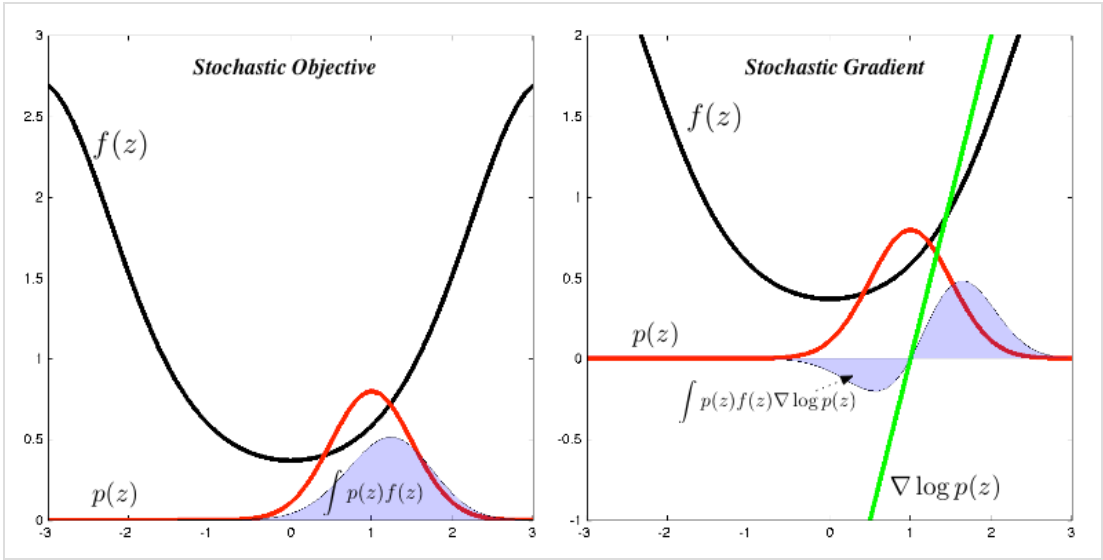
\includegraphics[scale=0.5]{gradient_change}
\caption{梯度變化}
\end{center}
\end{figure}
 讓我們導出該表達式,並探討它對我們的優化問題的影響。\\
 為此,我們將使用另一種普遍存在的技巧,一種概率恆等的技巧,在該技巧中,我們將表達式乘以1,該表達式由概率密度除以自身而形成。將特性技巧與對數導數技巧相結合,我們獲得了梯度的得分函數估計量:\\
$$\nabla_\theta \mathbb{E}_{p(z;\theta)}[f(z)]=\int\nabla_\theta p(z;\theta)f(z) dz$$
$$= \int \frac{p(z;\theta)}{p(z;\theta)}\nabla_\theta p(z;\theta)f(z) dz$$
$$=\int p(z;\theta)\nabla_\theta \log p(z;\theta)f(z) dz = \mathbb{E}_{p(z;\theta)}[f(z)\nabla_\theta \log p(z;\theta)]$$
$$=\int p(z;\theta)\nabla_\theta \log p(z;\theta)f(z) dz = \mathbb{E}_{p(z;\theta)}[f(z)\nabla_\theta \log p(z;\theta)]$$
$$\approx \frac{1}{S} \sum_{s=1}^{S}f(z^{(s)})\nabla_\theta \log p(z^{(s)};\theta) \quad z^{(s)}\sim p(z)$$\\
在這四行中發生了很多事情。在第一行中,我們交換了導數和積分。在第二行中,我們應用了概率身份技巧,這使我們能夠形成得分比, 然後使用對數導數技巧,用第三行中對數概率的梯度替換該比率。這在第四行給出了我們所需的隨機估計量,這是由蒙特卡洛計算的,方法是首先從p(z)提取樣本,然後計算加權梯度項。\\

更簡單的描述,我們有一些分佈 $p(x;\theta)$(我們使用了速記$ p \left( x \right)$ 來減少混亂),我們可以從中採樣(例如,這可能是高斯)。對於每個樣本,我們還可以評估score function f(x),該函數將樣本作為樣本並給出標量值。該方程式告訴我們,如果我們希望其樣本達到較高的分數(由f判斷),應該如何改變分佈(通過其參數θ),特別是,它看起來像:畫出一些樣本x,評估其分數f(x),並且對於每個x也評估第二項 $\nabla_\theta logp(x;θ)$,第二項是一個漸變向量為我們提供了參數空間中的方向,使分配給x的概率增加。換句話說,如果我們要在的方向上微移θ,$\nabla_\theta logp(x;θ)$,分配給x的新概率略有增加,朝這個方向移動,並將標量值加到上面$f(x)$。根據p(x)上的幾個樣本進行更新,則概率密度將朝著較高分數的方向移動,從而使得分較高的樣本更有可能出現。\\
\begin{figure}[hbt!]
\begin{center}
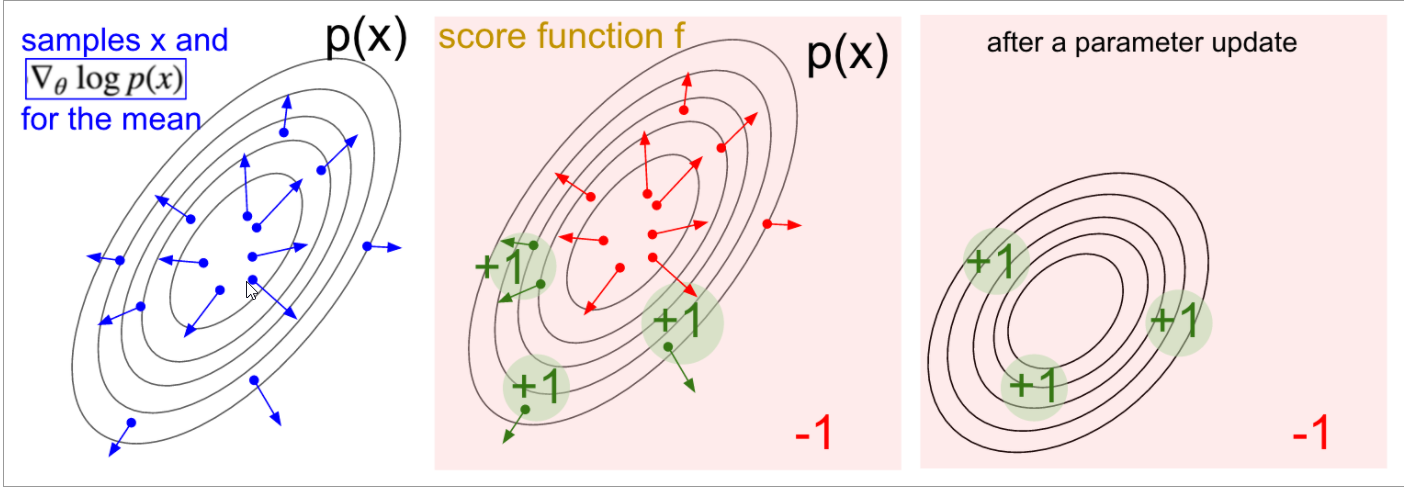
\includegraphics[scale=0.4]{figure}
\caption{Score Function可視圖}
\end{center}
\end{figure}

 Score function gradient estimator的可視化,左:高斯分佈及其中的一些樣本(藍點),在每個藍點上,我們還繪製了相對於高斯平均參數的對數概率的梯度,箭頭指示應微調分佈平均值以增加該樣本概率的方向。中間:某些得分函數的疊加,在某些小區域中除了+1之外,其他所有地方都給出-1,箭頭採用顏色區別,更新運用乘法運算,我們將平均所有綠色箭頭和紅色箭頭。右:更新參數後,綠色箭頭和反向紅色箭頭將向左移至底部。現在,根據需要,該分佈中的樣本將具有更高的預期分數。\\
\fi
\newpage

\chapter{訓練環境}
\section{OpenAI Gym}
 Gym 是用於開發和比較強化學習算法的工具包,他不對agent的結構做任何假設,並且與任何數據計算庫兼容,而可以用來制定強化學習的算法。這個環境具有共享的介面,使我們能用來編寫常規算法,也就能教導agents如何步行到玩遊戲。\\[6pt]

\section{Pong}
 取自 1977年發行的一款家用遊戲機ATARI 2600中的遊戲,內建於Gym,這是一個橫向的乒乓遊戲,左方是預設電腦玩家,右邊由使用者或是由訓練程式控制(圖.\ref{fig.pong})。在強化學習範例中,Pong與實體冰球機簡化後環境相似。\\
\begin{figure}[hbt!]
\begin{center}
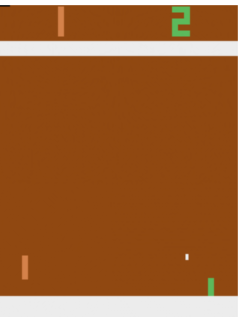
\includegraphics[height=8cm]{pong_gym}
\caption{\Large ATARI Pong}\label{fig.pong}
\end{center}
\end{figure} 

\newpage
\chapter{模擬環境}
%\renewcommand{\baselinestretch}{10.0} %設定行距
\section{模擬模型}
 在模擬的模型上,延用了學長設計的冰球機,並進行了部分的設計變更,將原本的人機對打更改為機器對打,且因為搭配深度強化學習的訓練,所以將兩邊的擊球器都僅保留X軸向(左右)移動,而冰球則是使用原本設計。多虧了學長們所設計的冰球機模型,讓我們在運作上有問題時可以直接發問,設計變更的地方也可以快速完成。\\
\begin{figure}[hbt!]
\center
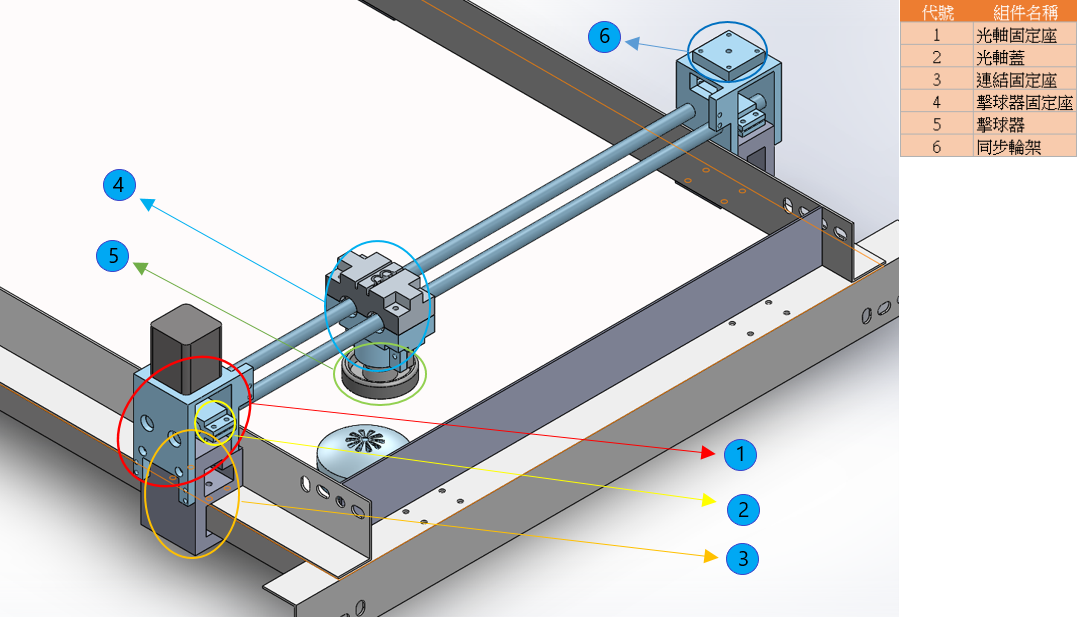
\includegraphics[width=13cm]{model}
\caption{\Large 組合圖}
\label{model}
\end{figure}

\qquad 將原本Y軸移動機構移除,並將其改為固定在特定位置上,此固定座設計是取代原本鎖在光軸固定坐上的(圖.\ref{model} 代號 1)Y軸皮帶固定座(圖.\ref{axialseat}),並使光軸固定座可以通過連結固定做鎖固於桌面,如(圖.\ref{connectSeat})。\\

\begin{figure}[hbt!]
\center
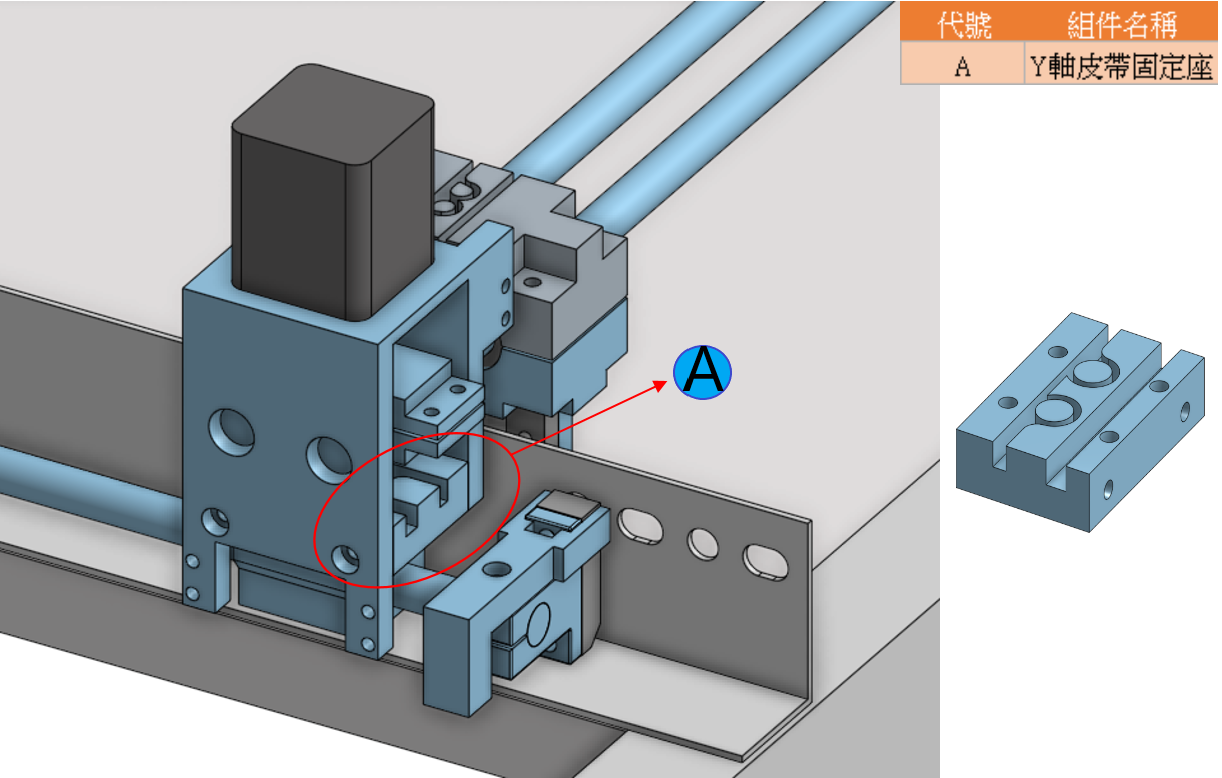
\includegraphics[width=8cm]{axialseat}
\caption{\Large Y軸皮帶固定座}
\label{axialseat}
\end{figure}

\begin{figure}[hbt!]
\center
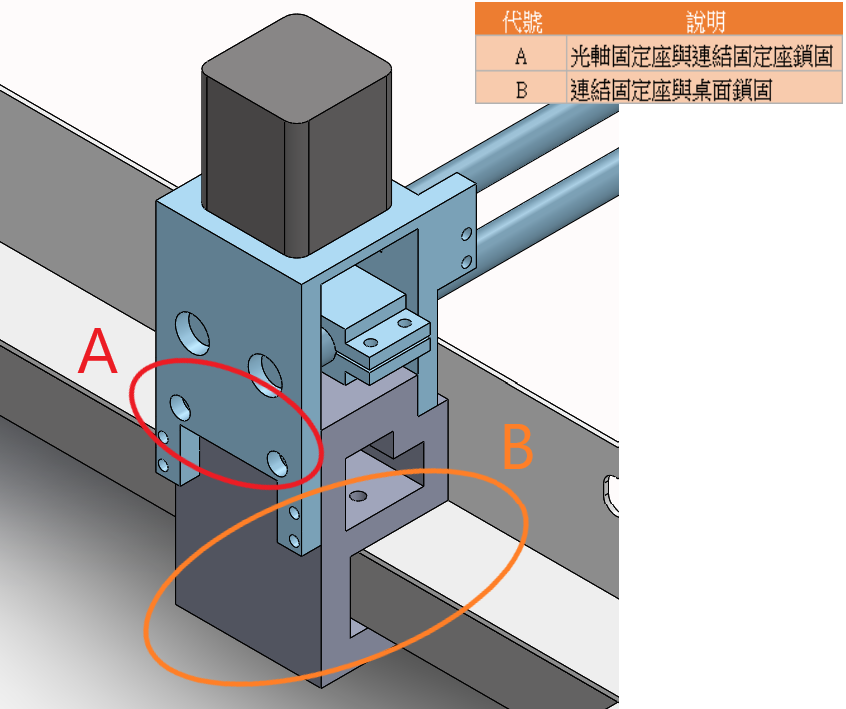
\includegraphics[width=8cm]{connectSeat}
\caption{\Large 連結固定座}
\label{connectSeat}
\end{figure}

\newpage
\qquad 分別在擊球器外側保留約冰球直徑1.5倍之區域作為得分判定區,如圖4.4中的紅色區域。\\
\section{CoppeliaSim模擬}
 CoppeliaSim是具有集成開發環境的機器人模擬器,基於分佈式控制體系架構,可以通過嵌入式腳本,插件,ROS或BlueZero節點,RemoteAPI客戶端或自定義解決方案進行模型控制。\\
 \begin{figure}[hbt!]
\center

\includegraphics[width=11cm]{CoppeliaSim}
\caption{\Large CoppeliaSim Logo}
\end{figure}

且CoppeliaSim中,控制器可以用C / C ++、Python、Java、Lua、Matlab或Octave編寫。\\
\subsection{使用原因}
 本專題之最終目標是希望可以在虛擬環境中進行深度強化學習來訓練機器對打,通過虛擬環境中的模擬後,可以更直接地看到深度強化學習訓練的狀況,且因為在虛擬環境中不會有金費的支出,所以可以不斷的重複模擬直到模擬達到最佳的狀態,除此之外CoppeliaSim的虛擬環境更接近真實環境,基於以上原因,所以使用了CoppeliaSim開發。\\
\subsection{RemoteAPI}
 RemoteAPI(Remote Application Programming Interface)是CoppeliaSim API框架的一部分。它允許CoppeliaSim與外部應用程序之間的通訊,是跨平台並支持服務調用和雙向數據流。有兩個不同的版本/框架分別為:Remote API 和The B0-based remote API。\\
\subsection{常用功能}
\begin{enumerate}
\item 以下為簡易功能說明:
\begin{figure}[hbt!]
\center
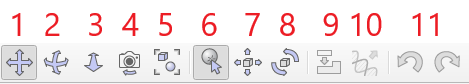
\includegraphics[width=11cm]{toolBar}
\caption{\Large CoppeliaSim 工具列}
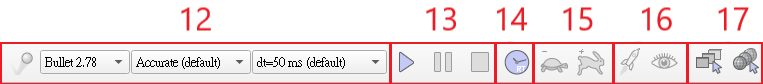
\includegraphics[width=13cm]{toolBar2}
\caption{\Large CoppeliaSim 工具列(續)}
\end{figure}
\begin{table}[hbt!]
\center
\large
\setlength{\tabcolsep}{0.75cm}{
\begin{tabular}{|c|c|c|c|}
\hline  代號 & 功能說明 & 代號 & 功能說明\\
\hline  1 &畫面平移& 10 &複製所有設定\\
\hline  2 &畫面旋轉& 11 &回復/取消回復\\
\hline  3 &畫面縮放&12&模擬設定\\
\hline  4 &畫面視角&13&開始/暫停/停止 模擬\\
\hline  5 &畫面縮放至適當大小&14&即時模擬切換\\
\hline  6 &選取物件&15&模擬速度控制\\
\hline  7 &移動物件&16&線程渲染/視覺化\\
\hline  8 &旋轉物件&17&場景/頁面 選擇\\
\hline  9 &加入/移出 樹狀結構&&\\
\hline 
\end{tabular}}
\caption{\Large 功能說明}
\end{table}
\newpage
%\item 模擬執行\\%
\end{enumerate}
\section{影像處理}

\qquad 在影像處理中我們主要使用了Python套件中的OpenCV(全稱:Open Source Computer Vision Library),並搭配其他套件或模組進行了影像處裡,藉此來取得訓練神經網路訓練時所需的資訊。\\
\begin{figure}[hbt!]
\center

\includegraphics[width=10cm]{pythonCVlogo}
\caption{\Large OpenCV 及Python logo}
\end{figure}

\subsection{CoppeliaSim中的Vision sensor(視覺傳感器)}
 CoppeliaSim的視覺傳感器輸出的影像是以每個像素中以RGB三個位元組所組成的,舉例來說:在CoppeliaSim中視覺傳感器取出畫面像素為512*256,則我們會接收到(512*256)像素*3=393,216個資料,是一筆相當大的資料,所以在影像處理上會消耗掉大量的資源。\\

\subsection{影像辨識}
 透過CoppeliaSim中的Vision sensor接收場景影像並輸出後,便可以開始進行影像辨識的處理。\\
\begin{enumerate}
\item RGB與HSV的轉換[\ref{RGBtoHSV}]\\
RGB即光的三原色Red(紅)Green(綠)Blue(藍),HSV則是一種將RGB色彩模型中的點在圓柱坐標系中的表示法,HSV分別表示Hue(色相)、Saturation(飽和度)、Value(明度),而會將RGB轉換為HSV是因為HSV相較於RGB可以更直接的判斷色彩、明暗和鮮豔度對於顏色過濾可以更方便定義出色彩範圍。\\
\begin{figure}[hbt!]
\center
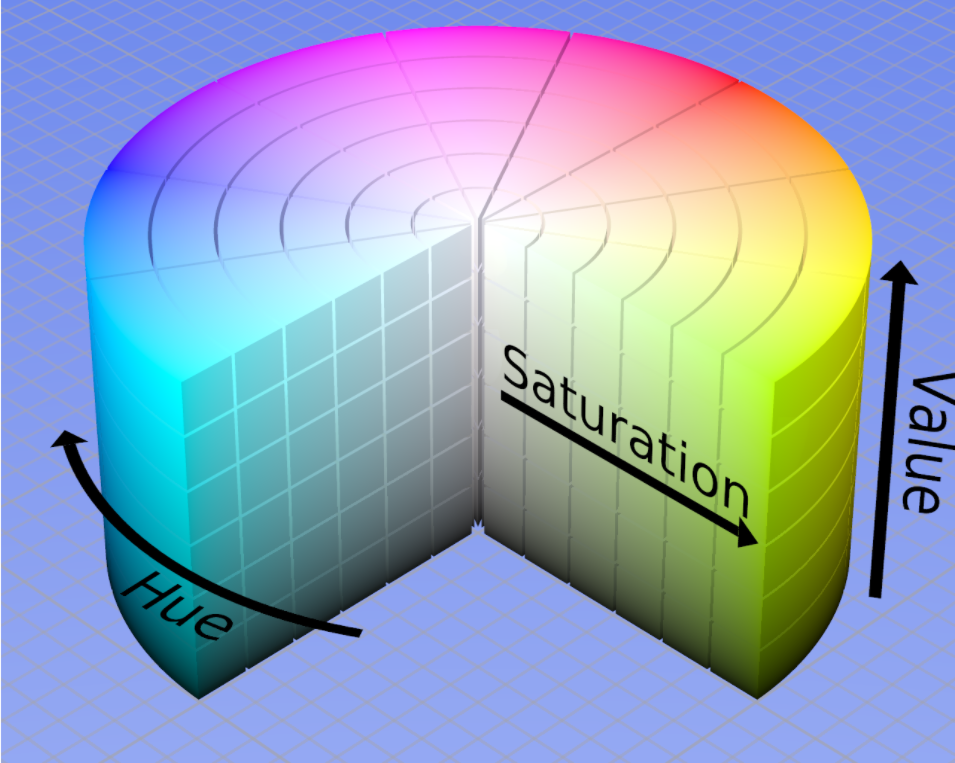
\includegraphics[width=10cm]{HSV}
\caption{\Large HSV色彩空間}
\end{figure}
\newpage
下列為RGB與HSV之間轉換的公式,首先是RGB轉為HSV,其中$max$及$min$分別為$(r,g,b)$中的最大與最小值:
$$h=\left\{\begin{matrix}
0^{\circ}, & \textrm{if}\ max=min\\ 
60^{\circ}+\frac{g-b}{max-min}+0^{\circ},& \textrm{if}\ max=r\;and\;g\geq \;b\\ 
60^{\circ}+\frac{g-b}{max-min}+360^{\circ}, & \textrm{if}\ max=r\;and\;g<  \;b\\ 
60^{\circ}+\frac{g-b}{max-min}+120^{\circ}, & \textrm{if}\ max=g\\ 
60^{\circ}+\frac{g-b}{max-min}+240^{\circ}, & \textrm{if}\ max=b
\end{matrix}\right.$$

$$s=\left\{\begin{matrix}
0, & \textrm{if}\,max=0\\ 
\frac{max-min}{max}=1-\frac{min}{max}, & \textrm{otherwise}
\end{matrix}\right.$$

$$v=max$$
接著是HSV轉為RGB:
$$\textrm{when}\,0\leq H< 360,0\leq S\leq 1,0\leq V\leq 1$$
$$C=V\times S$$
$$X=C\times (1-\left | (H/60^{\circ})\textrm{mod}2-1 \right |)$$
$$m=V-C$$

$$({R}',{G}',{B}')=\left\{\begin{matrix}
(C,X,0)& ,0^{\circ}\leq H< 60^{\circ}\\ 
 (X,C,0)& ,60^{\circ}\leq H< 120^{\circ}\\ 
 (0,C,X)& ,120^{\circ}\leq H< 180^{\circ}\\ 
 (0,X,C)& ,180^{\circ}\leq H< 240^{\circ}\\ 
 (X,0,C)& ,240^{\circ}\leq H< 300^{\circ}\\ 
 (C,0,X)& ,300^{\circ}\leq H< 360^{\circ}
\end{matrix}\right.$$


$$(R,G,B)=(({R}'+m)\times 255,({G}'+m)\times 255,({B}'+m)\times 255)$$

\item 顏色過濾\\
進行顏色過濾時,需要先定義出過濾顏色的上下限,在開始過濾後僅會保留介於上下界線範圍的影像,而介於上下限範圍之外的影像則會被剃除,如圖.\ref{filter}所示以上限(77,255,255)及下限(35,43,46)為例。\\
\begin{figure}[hbt!]
\center
\begin{minipage}[t]{0.48\textwidth}
\center
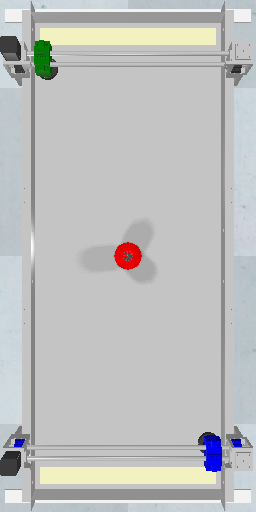
\includegraphics[width=6cm]{origin}
\caption{\Large 場景原圖}
\label{origin}
\end{minipage}
\begin{minipage}[t]{0.48\textwidth}
\center
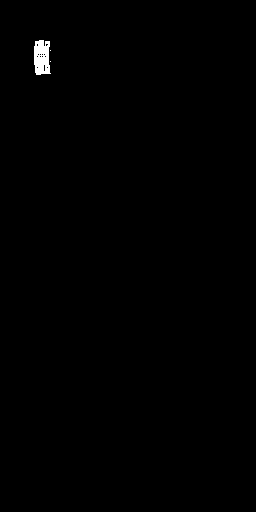
\includegraphics[width=6cm]{filter}
\caption{\Large 顏色過濾後的場景}
\label{filter}
\end{minipage}
\end{figure}


%\item 雜訊去除\\
%為了避免環境因素干擾,使影像產生雜訊並影響了影像辨識度,所以在雜訊的去除也是很重要的,

\end{enumerate}

\newpage
\chapter{伺服器}
 此專題採用 Ubuntu 20.04 版本作為我們的架設所使用作業系統,由於 Ubuntu 功能尤為繁多,以下說明重點只著重在專題製作所用到功能上。\\
 
 Ubuntu 作業系統是 Linux 系統的一個發行版,目前免費且開源,Ubuntu 基於 Debian發行版和 GNOME 桌面環境,其目標在於為一般使用者提供一個最新、穩定又主要以自由軟體建構而成的作業系統。\\
 
 其開發目的是為了使個人電腦變得簡單易用,它與其他基於 Debian 所發行的 Linux 版本更加接近 Debian 的開發理念,它主要使用自由、開源的軟體,而其他則帶很多閉源的軟體。\\
\section{Ubuntu 環境配置}
 在一開始會先使用套件管理系統 apt 指令去下載 Xorg , fluxbox , lxde 套件。Xorg 是 Ubuntu 操作系統的一個顯示服務器軟件包,它在被導入 Ubuntu 操作系統後會載入一系列的文件或軟件,這些都是跟顯示卡驅動,圖形環境庫相關的一些文件、軟件。Gnome ,kde,包括我們使用的 lxde 也需要 xorg 才能實現。而 Lxde 它的全名是 Lightweight X11 Desktop Environment ,是自由軟體桌面環境,其優點在於提供了輕量而快速的桌面環境,它比較重視實用、輕巧,除此之外它還可以在 Linux 平台執行。\\
 
 之後需選擇 display manager ( 顯示管理器 )的種類 ,Display manager 是操作系統 Ubuntu 的組件,其中登錄的動作即為 Display manager 負責。該操作系統中常見的類型有 gdm ,gdm3 , lightdm ,kdm ...。各類型的 Display manager 功能其實大同小異,差別在於外觀、操作、格式、複雜度和使用者感受等,可依使用者需求變更 ( 有些較為輕量,適合比較低階的運行器 )。選擇其中一個後繼續,之後可以切換更動 。\\

 再來是模組的導入,此處同樣用 apt 指令安裝:Pip , uwsgi , Nginx  , 以及 Git 。如果要從 Ubuntu 系統上安裝軟體,其中一種方式是 pip 。「pip 」是 "pip Installs Packages" 的縮寫,是一個用命令列作為基礎的套件管理系統,可以用它來安裝 python 的應用程式。而使用 Git 是因為在備份資料時, 可幫助使用者有效管理原始碼,而 github 就是由 Git 伺服器和網頁介面組成,用來當作放置原始碼的倉庫。\\
 
 另外 Nginx 和 uwsgi 是為拿來配合把 python 程式應用在網路上實現,並且把想要的結果使其能在網路實時觀看操控結果之反饋。\\
\section{Oracle VM VirtualBox 介紹}
 假使建構虛擬環境時需要在同一主機使用不同電腦作業系統環境,則可使用「虛擬機器工作站」— Oracle VM VirtualBox 。\\

 選擇 Oracle VM VirtualBox    是為了因應當要使用不同作業系統 ( 比如本機與虛擬環境不同作業系統  ) 且不想與其資料存放時共用一個硬碟 ( 無多餘硬碟 , 不想硬碟之間有資料重疊 ... ) 時,即可使用其軟體做練習,降低操作失誤帶來的成本,而此軟體目前為免費,並隨時會更新,另外其特色有 :\\  
\begin{itemize}


\item 只要自備作業系統 ( 光碟片 , ISO映像檔 ) ,即可在啟動 Oracle VM VirtualBox  後直接開啟要操作的執行檔 ( 作業系統 ),不必再把主機本身重新關機,當然開啟多個作業系統之間也有共通性,可直接從視窗A做網路、檔案分享、複製貼上等動作到視窗B。\\
\item 除了作業系統裡面的執行,還可在其中練習磁碟分割、格式化以及 BIOS 啟動等 ( 但是未支援USB啟動 ) 。\\
\item 空間的佔用上並不是真實佔用空間,而是依據使用者的操作而變化 ( 使用者用多少就是多少 )。相對的,使用者雖然一開始設定該虛擬電腦的記憶體大小與硬碟空間是實時依據操作者決定,但終究還是佔掉電腦效能,所以 VirtualBox 的效能還是依據電腦本身的硬體配備。為了配置網路,首先在:
\begin{enumerate}
\item File / Preferences / Network  位置,新增一個或右鍵點擊現有的網路設定,填入該電腦網路設定 。
\item Settings / Network / Adapter 1 / Attached to: 該位置改成  Bridged Adapter
\end{enumerate}
\qquad 此處配置之比較 ( 取常用例子 ):NAT , Bridged , Internal , Host-only
\item NAT:最為基本之設定,主要讓該虛擬主機可連上網,但在與其他網路使用者互動時找不到該虛擬主機網路位址,外部網路也無法偵測,虛擬主機所有的網路請求都會把該來源視為宿主機的。
\item Host-only:虛擬主機被分配到一個網址,但是還是只有虛擬主機運行的環境可訪問該網路位址
\item Internal:此種設定主要為虛擬主機彼此間的連線,它可向外部提供資料,但反之則不行。
\item Bridged:在與其宿主機的網卡設定橋接與設定好外部網路位址後,可被外部網路訪問。
\end{itemize}
\newpage
\section{Web server}
 Nginx 是提供 web 相關服務的伺服器 ( Web server ),除了是高效能的 HTTP ( HTTPS ) 服務器外,還可處理靜態資源 , 負載平衡 , 代理等工作。代理工作為根據不同域名轉發到 Application Server 的不同 port 上去處理 ,其中又分正向和反向,正向代理為 clinet 端發送 request 經由 porxy server 再到目標網站,反向則反之。正向代理操作中 server 只知道 proxy server  給他 request , 不知道 client 是誰,而相同地反向代理則是 client 只知道 proxy server 給他 responses , 不知道 server 是誰。正向代理隐藏真實 Client,反向代理隱藏真實 Server。另外在高流量的狀況下,需要多個 Application Server 來分擔流量,負載平衡就是負責 request 的分發,決定 request 要被分到哪一個 Application Server 處理 。而關於處理靜態資源 ,Nginx 與 Apache 等 Web Server 處理靜態資源的能力是遠遠高於 Application Server 的。\\
\begin{figure}[hbt!]
\begin{center}
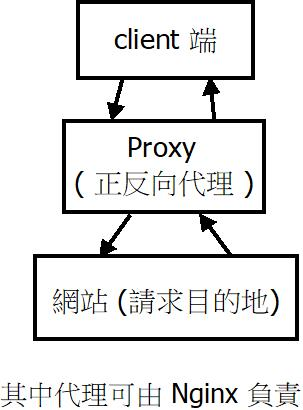
\includegraphics[scale=0.74]{clientProxy}
\caption{\Large clientProxy}\label{clientProxy}
\end{center}
\end{figure}

\section{Nginx}
\hspace{-1.7em} 網路設定:\\
 首先要修改網路設定檔,而其設定檔放在/etc/netplan目錄下的yaml檔。其中需更改的設定:
\begin{enumerate}
\item addresses:為靜態 IP,可以是IPV4或IPV6。
\item gateway:即為該電腦之閘道器。
\item nameservers:該電腦之DNS服務器。
\end{enumerate}

 WSGI(Python Web Server GateWay Interface)為一種用在Python語言上的規範,用來規範Web Server與Web Application之間如何溝通。而uWSGI同為實現了WSGI、uwsgi、http協議等的Web server,通常用於接收前端伺服器轉發的動態請求並轉發給Web Application。前者可以使用Nginx提供的https協定,且同上表述中Nginx的靜態資源處理能力較佳所以也能將靜態資源轉給其處理。\\
 
Nginx的主要設定檔nginx.conf可藉由include指令添加其他nginx設定檔的設定去擴增不同域名的設定,常見的設定有 :
\begin{enumerate}
\item 預設:
\begin{lstlisting}[caption=\Large nginx預設]
  reciveAPP {
    server localhost:5000;
    server localhost:5001;
}

server {
    listen 80;
    listen [::]:80;
    server_name SERVER_IP;
    root /home/hostname;

    location / {
            uwsgi_pass http://api/;
            include uwsgi_params;
    }
\end{lstlisting}

\newpage
\item 負載平衡LoadBalance:
\begin{lstlisting}[caption=\Large load balance設定]
  reciveAPP {
        ip_hash;
        server localhost:5000;
        server localhost:5001;
}

server {
    listen 80;
    listen [::]:80;
    server_name SERVER_IP;
    root /home/ryan;

    location / {
            uwsgi_pass 127.0.0.1:8000;
            include uwsgi_params;
    }
}
\end{lstlisting}
\end{enumerate}

 reciveAPP定義了將request proxy過去的應用,例子中server localhost語法代表可以請求proxy到分別監聽5000與5001 port的兩個應用,同時這個block可達到load balancer負載平衡的功能。\\
 
 server這個block則是定義了proxy server的相關設定,包括要監聽的port(listen 80為監聽所有IPV4位址,listen [::]80則為監聽所有IPV6位址)、規定哪些domain或ip的request會被 nginx server 處理(server\_ name)。\\
 
 location像是路由(routing)的概念,設定不同的path要對應到怎麼樣的設定。location中則是指對不同路徑的處理。\\
 
\begin{enumerate}
\item location:
\begin{lstlisting}[caption=\Large location設定]
  location / #匹配所有目錄

  location /static #匹配所有 /static 的開頭目錄
\end{lstlisting}
\end{enumerate}

 要達到load balancer透過一開始介紹的upstream block就可以達成,在上面的例子中,來自某個domain 80 port會被分配到port 5000或port 5001兩個應用中,達成用兩個應用去分擔request的負載平衡器。\\
 
 負載平衡裡的負載規則(ip\_hash )某個request要被導倒哪個應用去處理有不同規則,每個規則都有各自適合使用時機,以下簡單介紹幾個常見的規則:\\

\begin{enumerate}
\item round-robin(預設)輪詢方式:也就是將請求輪流按照順序分配給每一個 server。假設所有伺服器的處理效能都相同,不關心每臺伺服器的當前連線數和響應速度。適合於伺服器組中的所有伺服器都有相同的軟硬體配置並且平均伺服器請求相對均衡的情況。
不過也有另外一種可以設定權重的Weight Round Robin(加權輪詢方式),可以設定不同server的權重,例如以下範例:
\begin{lstlisting}[caption=\Large 設定不同 server 的權重]
  upstream myweb {
    server web1.dtask.idv.tw weight=3;
    server web2.dtask.idv.tw weight=2;
}
\end{lstlisting}
\item least-connected 最少連線:顧名思義為連線進來時會把Request導向連線數較少的Server。
\item IP-hash依據Client IP來分配到不同台Server:通過一個雜湊(Hash)函式將一個 IP 地址對映到一臺伺服器。先根據請求的目標IP地址,作為雜湊鍵(Hash Key)從靜態分配的散列表找出對應的伺服器。除非斷線或IP變動,否則同個IP的請求都會導入到同一個 server。
\end{enumerate}
  uWSGI設定(uwsgi\_ini ):
 \begin{enumerate} 
 \item wsgi-file:主要運行的py檔案
 \item http,socket,http-socket:端口設定,假使有使用到 前端服務器(如Nginx)時,不能用http設定,因uwsgi協議為HTTP,而Nginx使用傳輸協議為TCP,兩者不能互通。
 \begin{lstlisting}[caption=\Large 簡易uwsgi指令啟動]
  uwsgi --http:9000 --wsgi-file APP.py 
\end{lstlisting}
 \item processes、threads:工作序,processes為進程,threads為線程,下方設定為每條近程有兩條線程。
 \begin{lstlisting}[caption=\Large 加入工作程序uwsgi指令啟動]
  uwsgi --http:9000 --wsgi-file APP.py --processes 4 --threads 2
\end{lstlisting}
\item chdir:此項是為了正確的加載模組/檔案 \\
整體快速配置(這裡儲存成一個.ini文件,其他還有YAML、JSON、XML格式等):
\begin{lstlisting}[caption=\Large 將uwsgi指令啟動動作設定成一個啟動檔]
  [uwsgi]
socket = :9000
processes = 4
threads = 2
chdir = location/to
wsgi-file = location/to/file
\end{lstlisting}
此項還可加上status:此項為查看uWSGI內部的輸出數據\\
\begin{lstlisting}[caption=\Large status]
  -- status 127.0.0.1:9001
\end{lstlisting}
實現之通訊流程 

\begin{figure}[hbt!]
\begin{center}
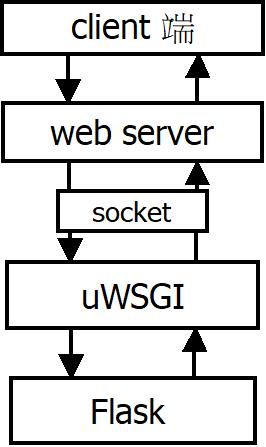
\includegraphics[scale=0.74]{clientToflask}
\caption{\Large client To flask}\label{clientToflask}
\end{center}
\end{figure}
 \end{enumerate}
\section{Flask}
 
 如同以上所述,建立Flask框架的同時需選擇反向代理伺服器(這裡我們選擇了Nginx)來負責網頁請求和結果的回覆,同時還需要一個實現WSGI通信協議的伺服器(我們選擇了 uWSGI)來負責接收代理伺服器的請求後Flask轉發及接收訊息,再轉發回去(代理伺服器)。\\
 
\begin{figure}[hbt!]
\begin{center}
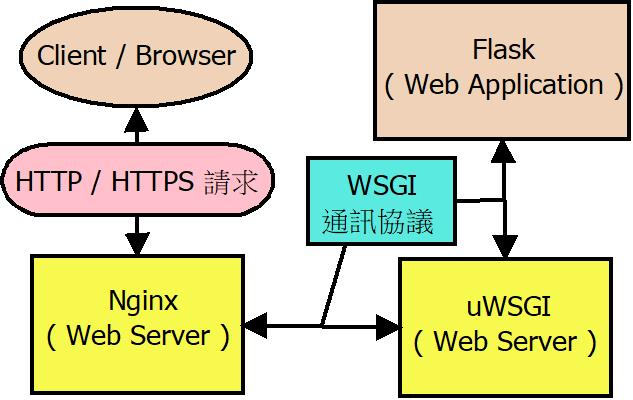
\includegraphics[scale=0.74]{total}
\caption{\Large total}\label{total}
\end{center}
\end{figure}

\chapter{機器學習的訓練與模擬控制結果}
\section{訓練模型的基礎概念}
 訓練模型的原型是實體冰球機的機電系統,由於要訓練強化學習,所以需要將模型簡化至最簡潔的方式進行訓練,並取Open AI Gym的環境當作最簡化的訓練模型。由於強化學習是一種最佳化控制的方式,因此將Gym的Pong畫面當作輸入,輸出為擊錘移動方向,藉由調整當中的權重、偏差等參數,將參數調配到最優狀態。將可行的訓練方式套用到CoppeliaSim進行虛擬環境的訓練,並且可將訓練結果套用到實機進行運用。\\
\section{訓練模型的選用}
 利用Gym的環境訓練機器學習,以測試學習率、神經網路隱藏層的神經元個數、機器學習的啟動函數類型、訓練時影像大小等幾項參數與訓結果之間的關聯性,選用pyhton語言進行配置。剛開始我們運用Pygame模組來撰寫pong game的訓練環境,開始學習並了解Pygame的一些運用,嘗試建構出pong game場景(圖.\ref{fig.pong_pygame}),在基本功能編寫告一段落後,測試程式漏洞,發現對打時特定角度碰撞,球會超過擊錘的碰撞感測,導致出現球擊穿擊錘的現象。為了解決Pygame碰撞問題,做了幾種嘗試:修改Pygame的碰撞定義,更換碰撞感測的感測方式,問題依舊沒有顯著的改善,若增加過多的碰撞偵測點則會造成後續機器學習訓練時的運算負荷;另一種方法則是搭配pymunk的物理引擎模組使用(圖.\ref{fig.airhockey_pymunk}),使環境更符合實際物理現象,可加入碰撞、摩擦、力量大小、速度大小等可以個別設定和調用。當環境有了物理接下來就需要加入訓練所需的功能,如:訓練時的場景的即時影像畫面、即時獎勵回傳、該局結束時的場景重設和分數重置等功能。此時找到了Open AI Gym模組。\\
\begin{figure}[hbt!]
\begin{center}
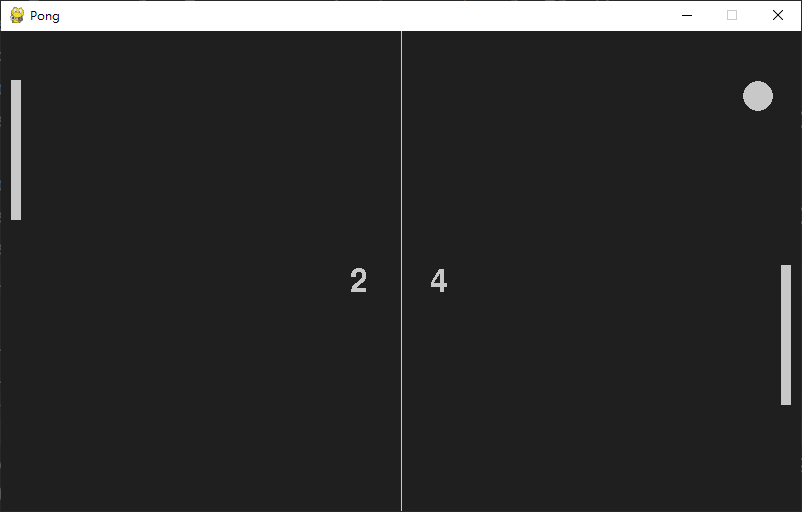
\includegraphics[width=12cm]{pong_pygame}
\caption{\Large Pygame模組編寫}
\label{fig.pong_pygame}
\end{center}
\end{figure}

\begin{figure}[hbt!]
\begin{center}
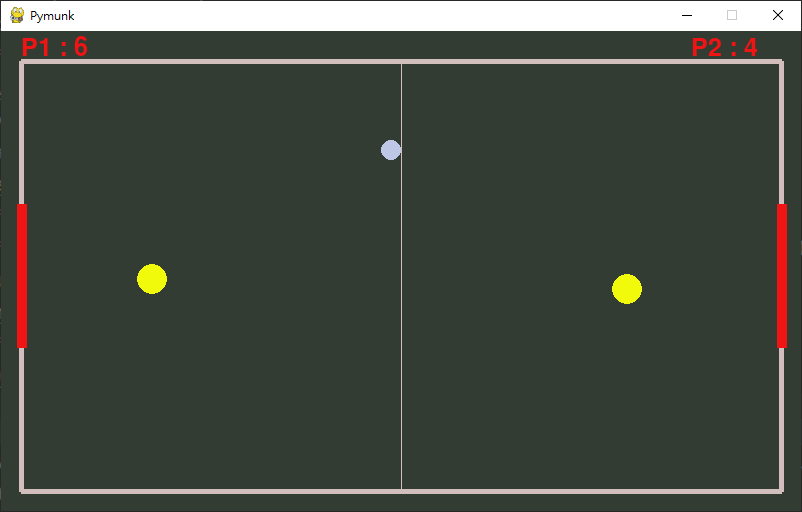
\includegraphics[width=12cm]{airhockey_pymunk}
\caption{\Large Pymunk模組編寫}
\label{fig.airhockey_pymunk}
\end{center}
\end{figure}
 \newpage %圖片空隙勿刪
 Open AI Gym裡面有十幾種訓練模型的環境,提供機器學習做訓練的環境。由於我們的訓練模型是pong game,在Gym模組裡面剛好有訓練模型,因此使用Gym模組相對於使用Pygame和pymunk的搭配來的方便,而且後續要在CoppeliaSim模擬環境模擬時也有套件可搭配使用,可簡化功能和訓練時所需的環境模型和訓練功能的程式編寫,另一方面自寫場景需要測試場景的漏洞,使用Gym可以節省檢查場景漏洞和修正的時間。\\
\section{訓練程式的運作}
 由於機器學習和影像處理需要大量的運算矩陣運算,因此如果只單獨透過Python本身運算比編譯語言執行的速度來的慢,所以使用Numpy程式庫來解決在Python環境矩陣運算速度慢的問題,以提升訓練機器學習時的運算效率。pickle是Python內部的序列化方式,主要是當機器學習訓練時可能因為一些原因需要暫時停止訓練,但為了讓已經停下的訓練再次重啟就需要透過pickle序列化的方式,將暫停前的訓練權重值透過pickle將其記錄下來,當訓練再次重啟時就可透過pickle.load讀取先前紀錄的pickle檔案就可回到當時暫停的狀態下繼續進行訓練。\\
 
 機器學習所運用的架構是強化學習並搭配神經網路來訓練機器學習,結合了強化學習不需要事先收集訓練資料、不需要特別教導,以及神經網路的非線性激活函數的計算和參數的記憶性。\\

\begin{figure}[hbt!]
\begin{center}
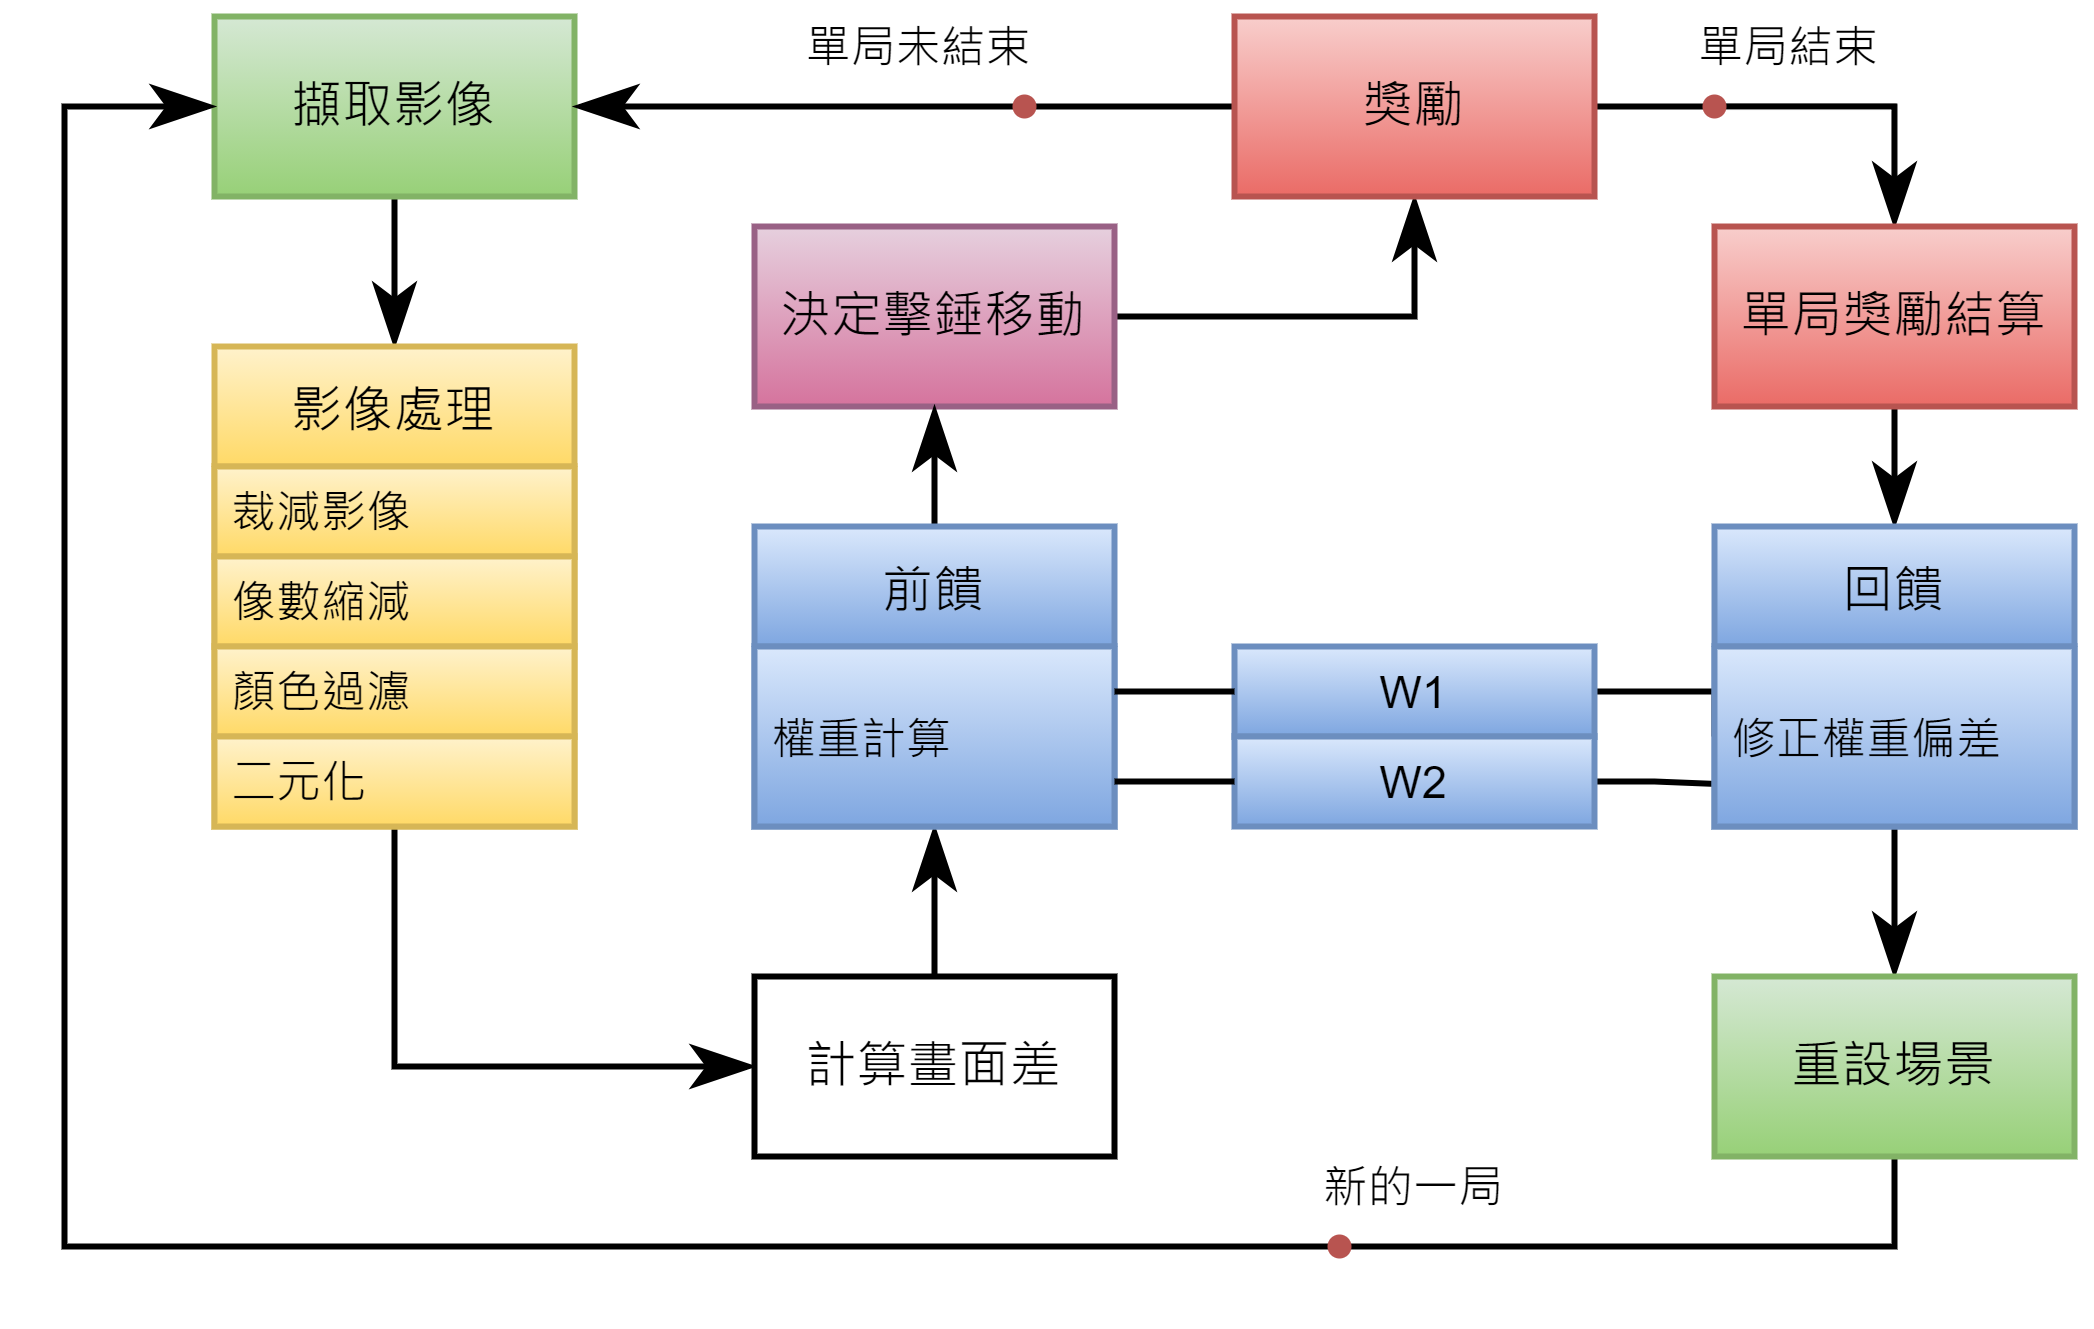
\includegraphics[width=15cm]{強化學習訓練流程}
\caption{\Large 強化學習訓練流程}
\label{fig.強化學習程式流程}
\end{center}
\end{figure}
%-----------------------------%

%=---------圖片空隙勿刪--------=%
%-----------------------------%
程式訓練流程(圖.\ref{fig.強化學習程式流程}):\\
 擷取影像,將影像裁剪至實際遊戲範圍,並簡化像素以利提高訓練時的計算速度,減少運算時的負擔,過濾顏色只保留球與擊錘,並把取到的影像二元化,取兩幀畫面進行比較,掌握球與擊錘間的相對位置(畫面差),透過前饋:計算球在環境的狀態及擊錘移動的決策,畫面差透過W1權重來計算球在環境的狀態,透過W2權重並經過啟動函數(activation function)得出擊錘移動的決策。透過產生隨機值的方式來與擊錘移動決策值進行比較,判定隨機值落在的區間來決定移動策略。計算discount reward及獎勵的加總。獎勵設定球若超過了對手,獎勵為+1;如果錯過球,則獎勵為-1;其餘狀態獎勵為0。\\

 在單局結束時,紀錄下該局累積下來的經驗,亦是紀錄該局所修正出來的參數而進行獎勵計算、log probability、RMSprop優化率減因子和反饋(back propagation),當訓練次數到達指定次數會以pickle做紀錄,存下的數據可再次導入模型進行實際運用,或是當程式中斷後可重新匯入進行訓練。比較持續訓練與中斷後重新匯入訓練的差異,測試算法版本為Pong2,MSE代表均方誤差值,pong2\_ r表示中斷後重新匯入的訓練數據,pong2與pong2\_ r標示個別表示該訓練每局分數的紀錄,pong2 MSE與pong2\_ r MSE標示個別表示該訓練均方誤差值紀錄(圖.\ref{fig.比較中斷數據}) \\
\begin{figure}[hbt!]
\begin{center}
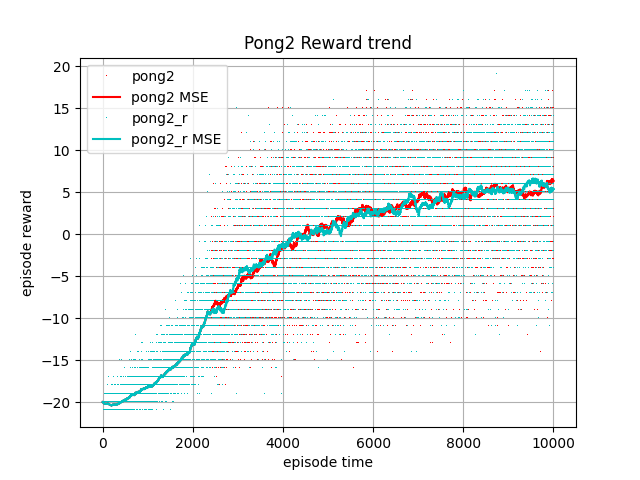
\includegraphics[width=15cm]{pong2_RvsNR}
\caption{\Large 比較中斷後訓練差異}
\label{fig.比較中斷數據}
\end{center}
\end{figure}

\section{訓練算法與參數比較}
 pong1版本是karpathy的pg\- pong.py的原始碼[\ref{R.pong1}],pong1.1原始碼則是schinger的pong\_ actor\- critic/pg\- pong\- ac.py[\ref{R.pong1.1}],pong1.2的是修改pong1的學習率參數從0.001調整到0.0001,並且將裁切後80*80的影像改成75*80。pong2版本是etienne87的pg\- pong.py的原始碼[\ref{R.pong2}]修改的,將動作策略由上下上替換成停上下的模式,學習率也配合調整,由0.0001調至0.001。\\
 
 下圖(圖.\ref{fig.比較中斷數據})為這幾個版本的訓練趨勢的紀錄提供做比較,訓練次數(圖.\ref{fig.比較中斷數據}之水平軸)為3000局做比較,小點為每局積分總和(圖.\ref{fig.比較中斷數據}之垂直軸),線條為累積積分的均方誤差值,積分計算$-21$分代表對面得21分,即機器訓練所得分數-對面所得分數。訓練存在隨機性(Stochastic),因此每次訓練所得趨勢會有所差異。\\
\begin{table}[hbt!]
\center\large
\setlength{\tabcolsep}{0.75cm}{
\begin{tabular}{|c|c|c|c|}
\hline  版本名稱 & 標示顏色 & 啟動函數 & 參考來源\\
\hline  pong1 &  紅色 & sigmoid & [\ref{R.pong1}]\\
\hline  pong1.1 &  藍色 & sigmoid & [\ref{R.pong1.1}]\\
\hline  pong1.2 &  橘色 & sigmoid & [\ref{R.pong1}]\\
\hline  pong2 & 綠色 & softmax & [\ref{R.pong2}] \\
\hline
\end{tabular}}
\caption{\Large 版本標示}
\end{table}

\begin{figure}[hbt!]
\begin{center}
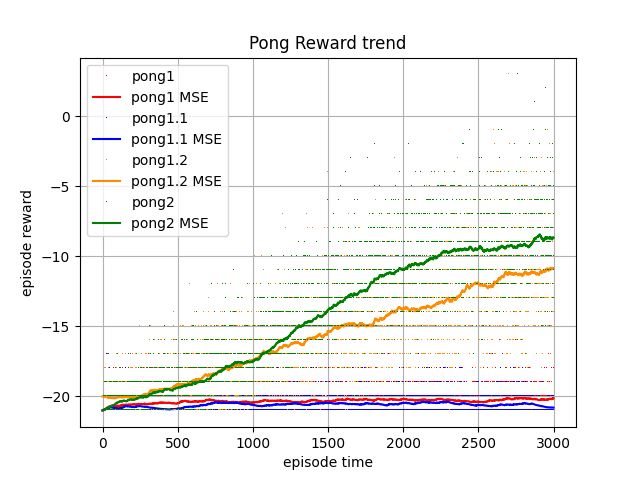
\includegraphics[width=15cm]{pong}
\caption{\Large 各版本差異}
\label{fig.各版本差異}
\end{center}
\end{figure}
觀察後發現,pong2版本的訓練結果得分最高,pong1.2的訓練結果為次高,pong1及pong1.1的版本沒有收斂,訓練對打的表現沒有進步的跡象,參數還需做調整及測試,pong2及pong1.2為主要選擇訓練演算法。接下來測試pong1的學習率調整成0.0001,pong1.2的學習率上調到0.001,以pong2版本當作對照(圖.\ref{fig.比較中斷數據}),同樣以3000次訓練當作參考依據,測試結果三者相當接近。因為訓練時間及設備限制,修正後的pong1與pong1.2版本所以擇一與pong2進行長時間訓練比較,因此選用pong1.2版本。

\begin{figure}[hbt!]
\begin{center}
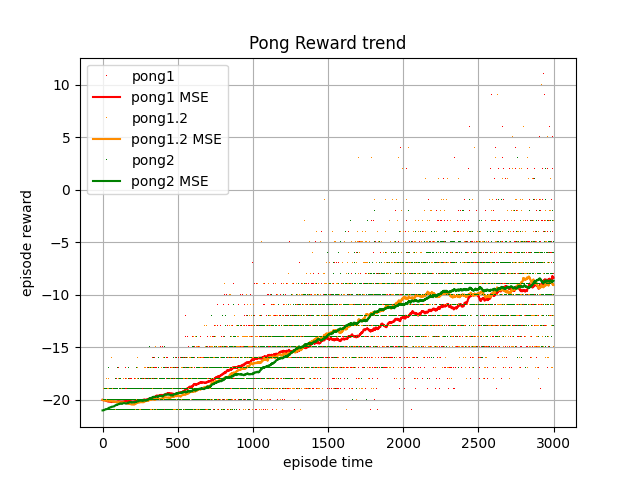
\includegraphics[width=15cm]{pong_test}
\caption{\Large pong1與1.2調整後數據比較}
\label{fig.調整後數據比較}
\end{center}
\end{figure}

\begin{flushleft}
電腦規格:\\
\end{flushleft}
\begin{enumerate}[1.]
\item 研究室桌上型電腦(長時間訓練所使用):\\
Windows10 專業版 2004\\
CPU:Intel i7-7700 3.60GHZ\\
RAM:16GB\\
GPU:NVDIA GTX1050
\item 個人筆記型電腦(3000次訓練數據為此設備訓練,短時間測試用):
Windows10 家用版 2004\\
CPU:Intel i7-8750H 2.20GHZ\\
RAM:8GB\\
GPU:NVDIA GTX1050 Ti\\

總訓練時數約336\textasciitilde 350小時(圖.\ref{fig.pong2與pong1.2長時間訓練比較}),pong2的數據均方誤差(MSE)數據較穩定,由於訓練中無法得知當下是處於數據波動的較優或較差的狀態,若要中斷訓練則有可能剛好處於波動的較差的狀態,因此選擇pong2的版本當作訓練算法較為穩定。
\end{enumerate}
\begin{figure}[hbt!]
\begin{center}
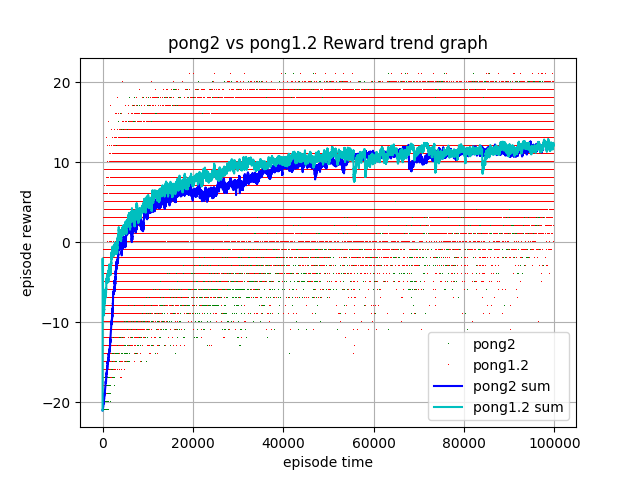
\includegraphics[width=15cm]{pong2_vs_pong1.2_reward}
\caption{\Large pong2與pong1.2長時間訓練數據}
\label{fig.pong2與pong1.2長時間訓練比較}
\end{center}
\end{figure}



\section{CoppeliaSim RemoteAPI}
在進行強化學習時主要是透過CoppeliaSim中的Remote API 函數來取得模擬場景中所需要的資訊,並在進行訓練後再回傳到CoppeloaSim做控制的動作。\\
\subsection{Remote API模組及動態連結函示庫}
在啟用RemoteAPI需要先準備以下三項模組和動態連結函示庫,並將此三項與預執行的程式放在同一目錄下:
\begin{itemize}
\item sim.py
\item simConst.py
\item remoteApi.dll、remoteApi.dylib 或 remoteApi.so (依序適用於:Windows、MacOS、Ubuntu)
\end{itemize}
sim.py及simConst.py為Python模組,其位於:\\
CoppeliaSim安裝目錄$\backslash$programming$\backslash$remoteApiBindings$\backslash$python$\backslash$python\\
remoteApi.dll為RemoteAPI動態連結函示庫,其位於:\\
CoppeliaSim安裝目錄$\backslash$programming$\backslash$remoteApiBindings$\backslash$lib$\backslash$lib$\backslash$作業系統\\
\subsection{Remote API埠使用}
Remote API是通過通訊埠取得環境資訊,在CoppeliaSim中預設埠號為19997,只有預設埠不需開啟特定場景就可進行通訊並控制所有功能,且在大量影像資料處理時可啟用多埠,使其中一個通訊埠用於影像處理,另一個則用於控制,新增的通訊埠需在安裝資料夾中的remoteApiConnections.txt加入需要的埠號。\\
\section{Open AI Gym自定義環境}
Open AI Gym可以支持我們以自己搭建的環境進行訓練,因此我們透過Gym並以CoppeliaSim虛擬環境中搭建的冰球機模型來完成訓練,而Gym所使用的環境參數就是由前述的Remote API來取得。Gym將環境抽象為一個類別(class)在該類別(class)中需分別定義以下參數來達成自定義環境的訓練。\\

\begin{enumerate}
\item init:初始化CoppeliaSim中的環境參數。
\item seed:用於設置環境變數。
\item make observation :用於設置環境場景中需觀察的值,如:擊錘位置、冰球位置...等。
\item make action:設置擊錘的移動速度。
\item step:訓練的主要邏輯,如:遊戲是否結束、reward函數返回值、環境觀察值...等。
\item reset:將環境重置。
\item render:可搭配OpenCV進行數據渲染。
\item close:釋放環境數據。\\
\end{enumerate}

\section{總結}
選擇適合的演算法,並找到適合的參數,透過訓練提升機器對打的能力,訓練的時間越長,學習對打的成效越好,但訓練後期進步的幅度趨緩,因此得評估訓練的時間長度以符合整體效益。在模擬環境中利用RemoteAPI建置了跨平台控制,並運用CoppeliaSim中視覺傳感器所取得之影像透過OpenCV加以處理便於輔助玩家進行對打,在程式中則使用OpenCV處理及簡化過的影像進行擊錘移動的計算,將計算後得出的結果回傳到CoppeliaSim中的環境,使擊錘做出對應的動作。
\newpage

\chapter{未來研究建議}
本專題已建立2D環境的算法與訓練數據,並將實體系統導入虛擬環境,建立跨平台控制(RemoteAPI)及輔助對打系統,後續可透過建立虛擬環境的訓練程式進行虛擬訓練,完成虛擬訓練後可導入實體機電系統,將對打系統實體化,架設伺服器提供網際介面,提供網際控制、即時觀看對打影像等功能。
\begin{figure}[hbt!]
\begin{center}
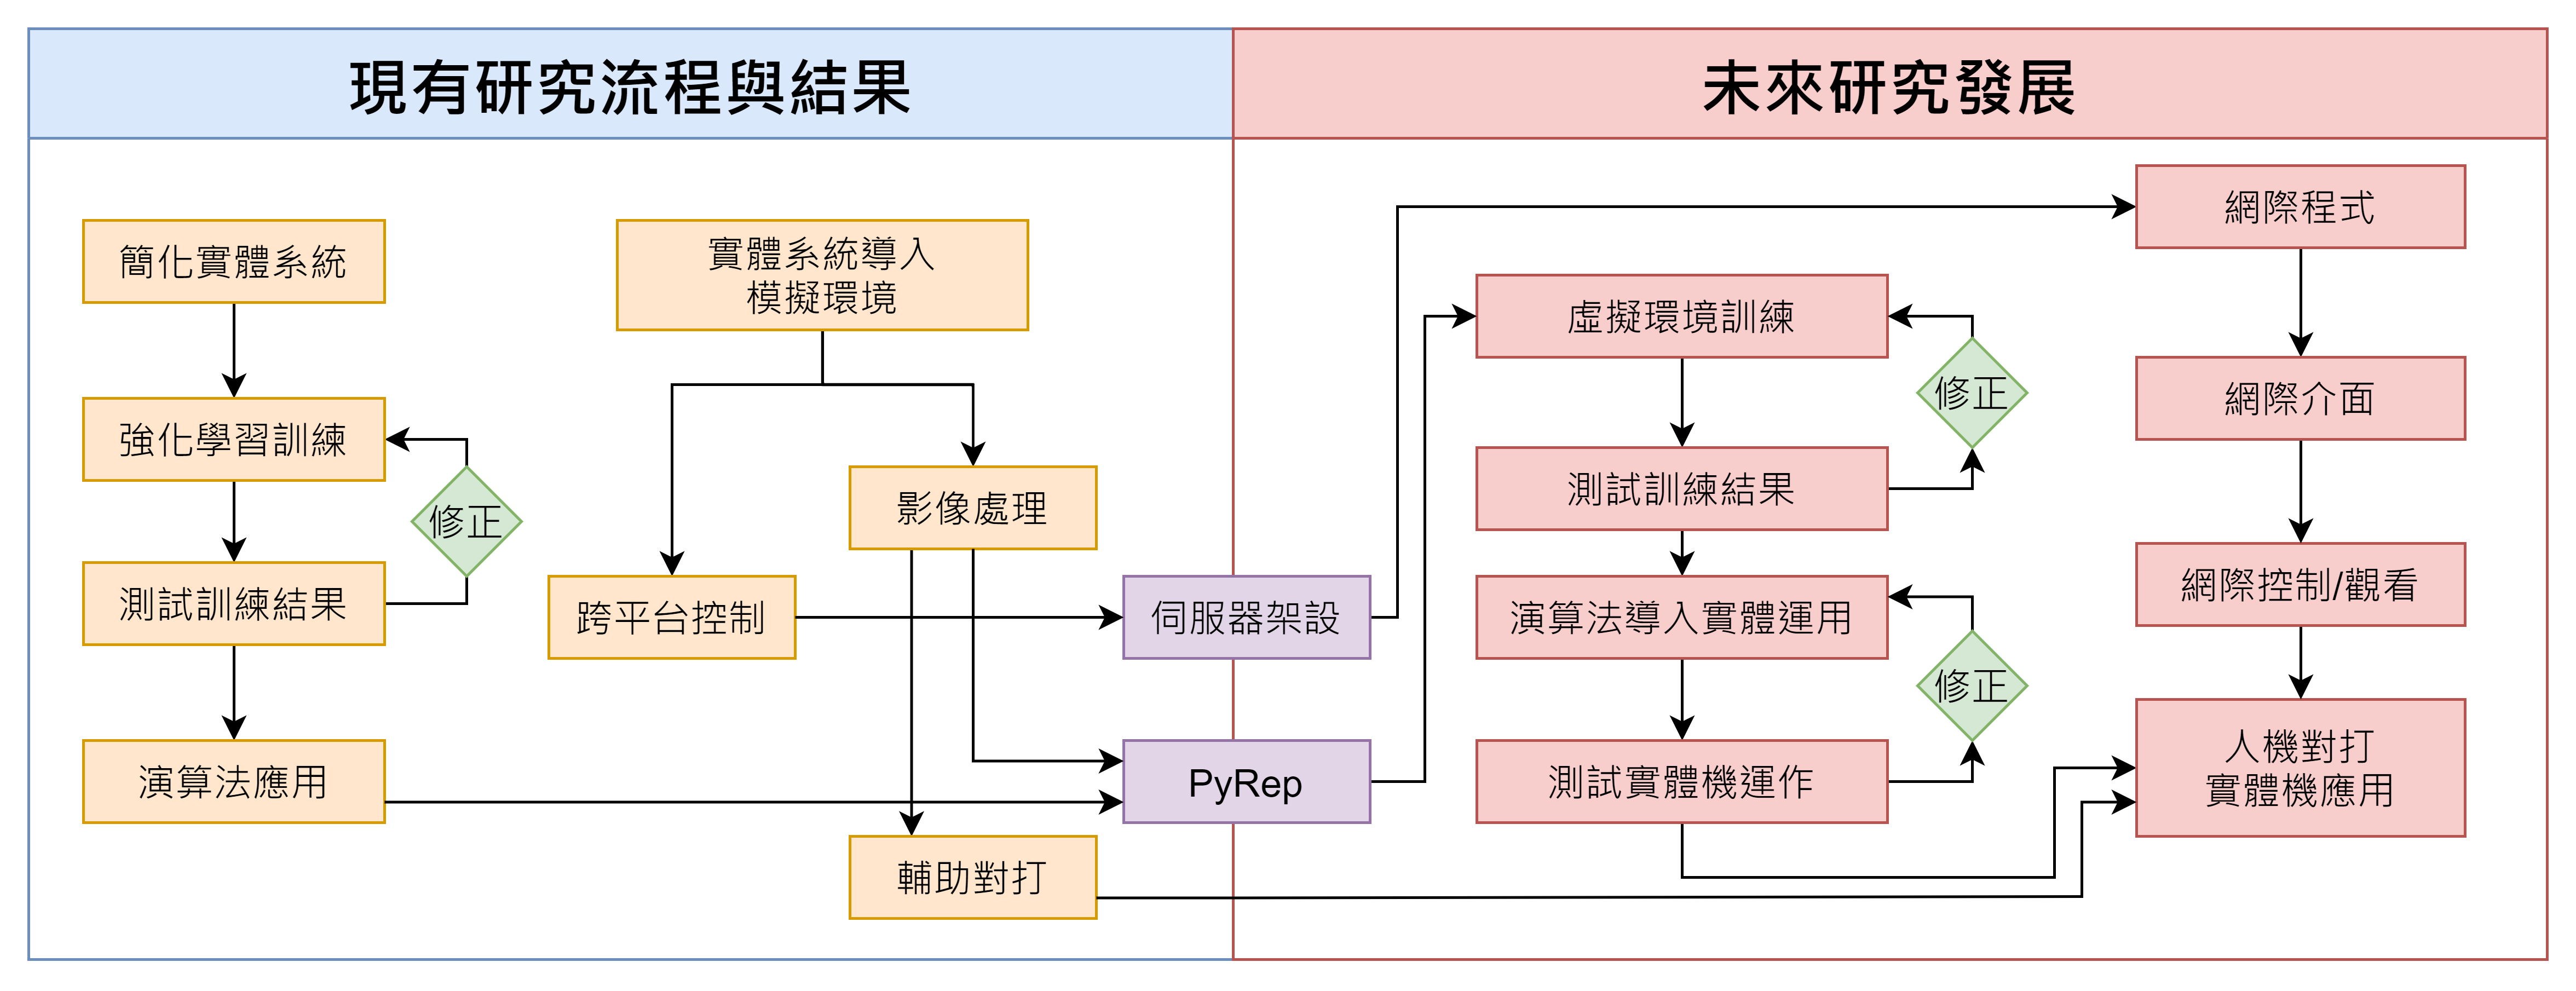
\includegraphics[width=16cm]{現有研究流程與未來展望}
\caption{\Large 現有研究流程與未來展望}
\label{fig.現有研究流程與未來展望}
\end{center}
\end{figure}



%=---------------------參考文獻----------------------=%
\addcontentsline{toc}{chapter}{參考文獻} %新增目錄名稱
\newpage
\renewcommand\bibname{參~考~文~獻}
\begin{thebibliography}{99}  % 參考文獻印出之編號最寬為兩個字母寬
\bibitem 1\href{https://towardsdatascience.com/adam-latest-trends-in-deep-learning-optimization-6be9a291375c}{https://towardsdatascience.com/adam-latest-trends-in-deep-learning-optimization-6be9a291375c}
\bibitem 2\href{https://towardsdatascience.com/derivative-of-the-sigmoid-function-536880cf918e}{https://towardsdatascience.com/derivative-of-the-sigmoid-function-536880cf918e}
\bibitem 3\href{http://www.incompleteideas.net/book/RLbook2020.pdf}{http://www.incompleteideas.net/book/RLbook2020.pdf}
\bibitem 4\href{https://medium.com/change-the-world-with-technology/policy-gradient-181d43a24cf5}{https://medium.com/change-the-world-with-technology/policy-gradient-181d43a24cf5}
\bibitem 5\href{https://livebook.manning.com/book/grokking-deep-reinforcement-learning/chapter-11/v-11/38}{https://livebook.manning.com/book/grokking-deep-reinforcement-learning/chapter-11/v-11/38}
\bibitem 6\href{http://ukko.life.nctu.edu.tw/~u0517047/usage.html}{http://ukko.life.nctu.edu.tw/~u0517047/usage.html}
\bibitem 7\href{https://lilianweng.github.io/lil-log/2018/04/08/policy-gradient-algorithms.html}{https://lilianweng.github.io/lil-log/2018/04/08/policy-gradient-algorithms.html}\label{R.Policy Gradient}
\bibitem 8\href{https://uupgrade.medium.com/python-那些年我們一起玩過的遊戲-三-打磚塊-d89b648896ca}{https://uupgrade.medium.com/python-那些年我們一起玩過的遊戲-三-打磚塊-d89b648896ca}
\bibitem 9\href{https://cvfiasd.pixnet.net/blog/post/275774124-深度學習激勵函數介紹}{https://cvfiasd.pixnet.net/blog/post/275774124-深度學習激勵函數介紹}
\bibitem 0\href{https://www.coppeliarobotics.com/helpFiles/}{https://www.coppeliarobotics.com/helpFiles/}
\bibitem 1\href{https://hackernoon.com/the-reason-behind-moving-in-the-direction-opposite-to-the-gradient-f9566b95370b}{https://hackernoon.com/the-reason-behind-moving-in-the-direction-opposite-to-the-gradient-f9566b95370b}\label{OGD}
\bibitem 2\href{https://ruder.io/optimizing-gradient-descent/}{https://ruder.io/optimizing-gradient-descent/}
\label{OGD2}
\bibitem 3\href{https://reurl.cc/43XjEL}{https://zh.wikipedia.org/wiki/HSL和HSV色彩空間}
\label{RGBtoHSV}
\bibitem 4\href{https://reurl.cc/gzMm4N}{https://gist.github.com/karpathy/a4166c7fe253700972fcbc77e4ea32c5\# file-pg-pong-py}\label{R.pong1}
\bibitem 5\href{https://reurl.cc/95172Y}{https://github.com/schinger/pong\_ actor-critic/blob/master/pg-pong-ac.py}\label{R.pong1.1}
\bibitem 6\href{https://gist.github.com/etienne87/6803a65653975114e6c6f08bb25e1522}{https://gist.github.com/etienne87/6803a65653975114e6c6f08bb25e1522}\label{R.pong2}
%\bibitem 7\href
%\bibitem 8\href
%
%\bibitem 3\href{https://blog.csdn.net/Csdn_Darry/article/details/107142216}{https://blog.csdn.net/CsdnDarry/article/details/107142216}
\end{thebibliography}
\newpage
%=---------------附錄-----------------=%
\addcontentsline{toc}{chapter}{附錄} %新增目錄名稱
\begin{appendix}
\renewcommand{\thesection}{\bf 附錄 \Alph{section}}%設定標題名稱
\begin{center}
\fontsize{20pt}{0em}\selectfont\bf 附錄
\end{center}
\section*{LaTeX}
LaTex 為一種程式語言,支援標準庫 (Standard Libraries) 和外部程式庫 (External Libraries),不過與一般程式語言不同的是,它可以直接表述 Tex 排版結構,類似於 PHP 之於 HTML 的概念。但是直接撰寫 LaTex 仍較複雜,因此可以藉由 Markdown 這種輕量的標註式語言先行完成文章,再交由 LaTex 排版。
此專題報告採用編輯軟體為LaTeX,綜合對比Word編輯方法,LaTeX較為精準正確、更改、製作公式等,以便符合規範、製作。
 \begin{table}[htbp] %htbp代表表格浮動位置
			\centering%表格居中
			\caption{文字編輯軟體比較表}%表:標題
			\large%字體大小
			\label{tab_文字編輯軟體比較表:scale}
			\begin{tabular}{|c|c|c|c|c|c|c|}
			\hline
			\diagbox[width=5em]& 相容性 & 直觀性 & 文件排版 & 數學公式 & 微調細部\\ 
			\hline
			LaTeX 		&$\surd$&		&$\surd$&$\surd$&$\surd$\\
			\hline
			Word	 	&		&$\surd$&		&		&$\surd$\\
			\hline
			
			\end{tabular}
		\end{table}	

\begin{itemize} 
\item 特點:
\end{itemize}
\begin{enumerate}
\item 相容性:以Word為例會有版本差異,使用較高版本編輯的文件可能無法以較低的版本開啟,且不同作業系統也有些許差異;相比LaTeX可以利用不同編譯器進行編譯,且為免費軟體也可移植至可攜系統內,可以搭配Github協同編譯。
\item 文件排版:許多規範都會要求使用特定版型,使用文字編譯環境較能準確符合規定之版型,且能夠大範圍的自定義排定所需格式,並能不受之後更改而整體格式變形。
\item 數學公式呈現:LaTex可以直接利用本身多元的模組套件加入、編輯數學公式,在數學推導過程能夠快速的輸入自己需要的內容即可。
\item 細部調整:在大型論文、報告中有多項文字、圖片、表格,需要調整細部時,要在好幾頁中找尋,而LaTeX可以分段章節進行編譯,再進行合併處理大章節。
\end{enumerate}
\begin{figure}[hbt!]
\begin{center}
\includegraphics[width=10cm]{編譯流程}
\caption{\Large 編譯流程}
\label{fig.編譯流程}
\end{center}
\end{figure}
\end{appendix}
\section*{FFmpeg}
FFmpeg是一個開放原始碼的自由軟體,可以對音訊和視訊進行多種格式的錄影、轉檔、串流功能。在專題訓練過程中透過FFmpeg的視訊錄製的功能記錄對打影像來了解實際訓練狀況。
\newpage
\newpage
